\documentclass[]{article}
\usepackage{lmodern}
\usepackage{amssymb,amsmath}
\usepackage{ifxetex,ifluatex}
\usepackage{fixltx2e} % provides \textsubscript
\ifnum 0\ifxetex 1\fi\ifluatex 1\fi=0 % if pdftex
  \usepackage[T1]{fontenc}
  \usepackage[utf8]{inputenc}
\else % if luatex or xelatex
  \ifxetex
    \usepackage{mathspec}
  \else
    \usepackage{fontspec}
  \fi
  \defaultfontfeatures{Ligatures=TeX,Scale=MatchLowercase}
\fi
% use upquote if available, for straight quotes in verbatim environments
\IfFileExists{upquote.sty}{\usepackage{upquote}}{}
% use microtype if available
\IfFileExists{microtype.sty}{%
\usepackage{microtype}
\UseMicrotypeSet[protrusion]{basicmath} % disable protrusion for tt fonts
}{}
\usepackage[margin=1in]{geometry}
\usepackage{hyperref}
\hypersetup{unicode=true,
            pdftitle={TFG: La Inteligencia Artificial aplicada a la Inteligencia Emocional},
            pdfauthor={Jorge de Andrés},
            pdfborder={0 0 0},
            breaklinks=true}
\urlstyle{same}  % don't use monospace font for urls
\usepackage{color}
\usepackage{fancyvrb}
\newcommand{\VerbBar}{|}
\newcommand{\VERB}{\Verb[commandchars=\\\{\}]}
\DefineVerbatimEnvironment{Highlighting}{Verbatim}{commandchars=\\\{\}}
% Add ',fontsize=\small' for more characters per line
\usepackage{framed}
\definecolor{shadecolor}{RGB}{248,248,248}
\newenvironment{Shaded}{\begin{snugshade}}{\end{snugshade}}
\newcommand{\AlertTok}[1]{\textcolor[rgb]{0.94,0.16,0.16}{#1}}
\newcommand{\AnnotationTok}[1]{\textcolor[rgb]{0.56,0.35,0.01}{\textbf{\textit{#1}}}}
\newcommand{\AttributeTok}[1]{\textcolor[rgb]{0.77,0.63,0.00}{#1}}
\newcommand{\BaseNTok}[1]{\textcolor[rgb]{0.00,0.00,0.81}{#1}}
\newcommand{\BuiltInTok}[1]{#1}
\newcommand{\CharTok}[1]{\textcolor[rgb]{0.31,0.60,0.02}{#1}}
\newcommand{\CommentTok}[1]{\textcolor[rgb]{0.56,0.35,0.01}{\textit{#1}}}
\newcommand{\CommentVarTok}[1]{\textcolor[rgb]{0.56,0.35,0.01}{\textbf{\textit{#1}}}}
\newcommand{\ConstantTok}[1]{\textcolor[rgb]{0.00,0.00,0.00}{#1}}
\newcommand{\ControlFlowTok}[1]{\textcolor[rgb]{0.13,0.29,0.53}{\textbf{#1}}}
\newcommand{\DataTypeTok}[1]{\textcolor[rgb]{0.13,0.29,0.53}{#1}}
\newcommand{\DecValTok}[1]{\textcolor[rgb]{0.00,0.00,0.81}{#1}}
\newcommand{\DocumentationTok}[1]{\textcolor[rgb]{0.56,0.35,0.01}{\textbf{\textit{#1}}}}
\newcommand{\ErrorTok}[1]{\textcolor[rgb]{0.64,0.00,0.00}{\textbf{#1}}}
\newcommand{\ExtensionTok}[1]{#1}
\newcommand{\FloatTok}[1]{\textcolor[rgb]{0.00,0.00,0.81}{#1}}
\newcommand{\FunctionTok}[1]{\textcolor[rgb]{0.00,0.00,0.00}{#1}}
\newcommand{\ImportTok}[1]{#1}
\newcommand{\InformationTok}[1]{\textcolor[rgb]{0.56,0.35,0.01}{\textbf{\textit{#1}}}}
\newcommand{\KeywordTok}[1]{\textcolor[rgb]{0.13,0.29,0.53}{\textbf{#1}}}
\newcommand{\NormalTok}[1]{#1}
\newcommand{\OperatorTok}[1]{\textcolor[rgb]{0.81,0.36,0.00}{\textbf{#1}}}
\newcommand{\OtherTok}[1]{\textcolor[rgb]{0.56,0.35,0.01}{#1}}
\newcommand{\PreprocessorTok}[1]{\textcolor[rgb]{0.56,0.35,0.01}{\textit{#1}}}
\newcommand{\RegionMarkerTok}[1]{#1}
\newcommand{\SpecialCharTok}[1]{\textcolor[rgb]{0.00,0.00,0.00}{#1}}
\newcommand{\SpecialStringTok}[1]{\textcolor[rgb]{0.31,0.60,0.02}{#1}}
\newcommand{\StringTok}[1]{\textcolor[rgb]{0.31,0.60,0.02}{#1}}
\newcommand{\VariableTok}[1]{\textcolor[rgb]{0.00,0.00,0.00}{#1}}
\newcommand{\VerbatimStringTok}[1]{\textcolor[rgb]{0.31,0.60,0.02}{#1}}
\newcommand{\WarningTok}[1]{\textcolor[rgb]{0.56,0.35,0.01}{\textbf{\textit{#1}}}}
\usepackage{graphicx,grffile}
\makeatletter
\def\maxwidth{\ifdim\Gin@nat@width>\linewidth\linewidth\else\Gin@nat@width\fi}
\def\maxheight{\ifdim\Gin@nat@height>\textheight\textheight\else\Gin@nat@height\fi}
\makeatother
% Scale images if necessary, so that they will not overflow the page
% margins by default, and it is still possible to overwrite the defaults
% using explicit options in \includegraphics[width, height, ...]{}
\setkeys{Gin}{width=\maxwidth,height=\maxheight,keepaspectratio}
\IfFileExists{parskip.sty}{%
\usepackage{parskip}
}{% else
\setlength{\parindent}{0pt}
\setlength{\parskip}{6pt plus 2pt minus 1pt}
}
\setlength{\emergencystretch}{3em}  % prevent overfull lines
\providecommand{\tightlist}{%
  \setlength{\itemsep}{0pt}\setlength{\parskip}{0pt}}
\setcounter{secnumdepth}{0}
% Redefines (sub)paragraphs to behave more like sections
\ifx\paragraph\undefined\else
\let\oldparagraph\paragraph
\renewcommand{\paragraph}[1]{\oldparagraph{#1}\mbox{}}
\fi
\ifx\subparagraph\undefined\else
\let\oldsubparagraph\subparagraph
\renewcommand{\subparagraph}[1]{\oldsubparagraph{#1}\mbox{}}
\fi

%%% Use protect on footnotes to avoid problems with footnotes in titles
\let\rmarkdownfootnote\footnote%
\def\footnote{\protect\rmarkdownfootnote}

%%% Change title format to be more compact
\usepackage{titling}

% Create subtitle command for use in maketitle
\providecommand{\subtitle}[1]{
  \posttitle{
    \begin{center}\large#1\end{center}
    }
}

\setlength{\droptitle}{-2em}

  \title{TFG: La Inteligencia Artificial aplicada a la Inteligencia Emocional}
    \pretitle{\vspace{\droptitle}\centering\huge}
  \posttitle{\par}
    \author{Jorge de Andrés}
    \preauthor{\centering\large\emph}
  \postauthor{\par}
      \predate{\centering\large\emph}
  \postdate{\par}
    \date{8 de Junio de 2019}


\begin{document}
\maketitle

Borramos el environment lo primero para siempre tenerlo limpio en la
ejecución:

\begin{Shaded}
\begin{Highlighting}[]
\KeywordTok{rm}\NormalTok{(}\DataTypeTok{list=}\KeywordTok{ls}\NormalTok{())}
\end{Highlighting}
\end{Shaded}

Importamos todas las librerías que vamos a ir necesitando:

\begin{Shaded}
\begin{Highlighting}[]
\CommentTok{#install.packages("ggplot2")}
\CommentTok{#install.packages("caret")}
\CommentTok{#install.packages("plyr")}
\CommentTok{#install.packages("wordcloud")}
\CommentTok{#install.packages("hexbin")}
\CommentTok{#install.packages("RColorBrewer")}
\CommentTok{#install.packages("corrplot")}
\CommentTok{#install.packages("FactoMineR")}
\CommentTok{#devtools::install_github("kassambara/factoextra")}
\CommentTok{#install.packages("factoextra")}
\CommentTok{#install.packages("nnet")}
\CommentTok{#install.packages("plotly")}
\CommentTok{#install.packages("class")}
\CommentTok{#install.packages("gmodels")}
\CommentTok{#install.packages("randomForest")}
\CommentTok{#install.packages("e1071")}
\CommentTok{#install.packages("ape")}
\CommentTok{#install.packages("cluster")}
\CommentTok{#install.packages("fpc")}
\CommentTok{#install.packages("devtools")}
\CommentTok{#devtools::install_github("vqv/ggbiplot")}
\CommentTok{#install.packages("party")}
\CommentTok{#install.packages("pROC")}

\KeywordTok{library}\NormalTok{(}\StringTok{"ggplot2"}\NormalTok{)}
\KeywordTok{library}\NormalTok{(}\StringTok{"caret"}\NormalTok{)}
\end{Highlighting}
\end{Shaded}

\begin{verbatim}
## Loading required package: lattice
\end{verbatim}

\begin{Shaded}
\begin{Highlighting}[]
\KeywordTok{library}\NormalTok{(}\StringTok{"plyr"}\NormalTok{)}
\KeywordTok{library}\NormalTok{(}\StringTok{"wordcloud"}\NormalTok{)}
\end{Highlighting}
\end{Shaded}

\begin{verbatim}
## Loading required package: RColorBrewer
\end{verbatim}

\begin{Shaded}
\begin{Highlighting}[]
\KeywordTok{library}\NormalTok{(}\StringTok{"hexbin"}\NormalTok{)}
\KeywordTok{library}\NormalTok{(}\StringTok{"RColorBrewer"}\NormalTok{)}
\KeywordTok{library}\NormalTok{(}\StringTok{"corrplot"}\NormalTok{)}
\end{Highlighting}
\end{Shaded}

\begin{verbatim}
## corrplot 0.84 loaded
\end{verbatim}

\begin{Shaded}
\begin{Highlighting}[]
\KeywordTok{library}\NormalTok{(}\StringTok{"FactoMineR"}\NormalTok{)}
\KeywordTok{library}\NormalTok{(}\StringTok{"factoextra"}\NormalTok{)}
\end{Highlighting}
\end{Shaded}

\begin{verbatim}
## Welcome! Related Books: `Practical Guide To Cluster Analysis in R` at https://goo.gl/13EFCZ
\end{verbatim}

\begin{Shaded}
\begin{Highlighting}[]
\KeywordTok{library}\NormalTok{(}\StringTok{"nnet"}\NormalTok{)}
\KeywordTok{library}\NormalTok{(}\StringTok{"plotly"}\NormalTok{)}
\end{Highlighting}
\end{Shaded}

\begin{verbatim}
## 
## Attaching package: 'plotly'
\end{verbatim}

\begin{verbatim}
## The following objects are masked from 'package:plyr':
## 
##     arrange, mutate, rename, summarise
\end{verbatim}

\begin{verbatim}
## The following object is masked from 'package:ggplot2':
## 
##     last_plot
\end{verbatim}

\begin{verbatim}
## The following object is masked from 'package:stats':
## 
##     filter
\end{verbatim}

\begin{verbatim}
## The following object is masked from 'package:graphics':
## 
##     layout
\end{verbatim}

\begin{Shaded}
\begin{Highlighting}[]
\KeywordTok{library}\NormalTok{(}\StringTok{"class"}\NormalTok{)}
\KeywordTok{library}\NormalTok{(}\StringTok{"gmodels"}\NormalTok{)}
\KeywordTok{library}\NormalTok{(}\StringTok{"randomForest"}\NormalTok{)}
\end{Highlighting}
\end{Shaded}

\begin{verbatim}
## randomForest 4.6-14
\end{verbatim}

\begin{verbatim}
## Type rfNews() to see new features/changes/bug fixes.
\end{verbatim}

\begin{verbatim}
## 
## Attaching package: 'randomForest'
\end{verbatim}

\begin{verbatim}
## The following object is masked from 'package:ggplot2':
## 
##     margin
\end{verbatim}

\begin{Shaded}
\begin{Highlighting}[]
\KeywordTok{library}\NormalTok{(}\StringTok{"e1071"}\NormalTok{)}
\KeywordTok{library}\NormalTok{(}\StringTok{"ape"}\NormalTok{)}
\KeywordTok{library}\NormalTok{(}\StringTok{"cluster"}\NormalTok{)}
\KeywordTok{library}\NormalTok{(}\StringTok{"fpc"}\NormalTok{)}
\KeywordTok{library}\NormalTok{(}\StringTok{"devtools"}\NormalTok{)}
\KeywordTok{library}\NormalTok{(}\StringTok{"ggbiplot"}\NormalTok{)}
\end{Highlighting}
\end{Shaded}

\begin{verbatim}
## Loading required package: scales
\end{verbatim}

\begin{verbatim}
## Loading required package: grid
\end{verbatim}

\begin{Shaded}
\begin{Highlighting}[]
\KeywordTok{library}\NormalTok{(}\StringTok{"party"}\NormalTok{)}
\end{Highlighting}
\end{Shaded}

\begin{verbatim}
## Loading required package: mvtnorm
\end{verbatim}

\begin{verbatim}
## Loading required package: modeltools
\end{verbatim}

\begin{verbatim}
## Loading required package: stats4
\end{verbatim}

\begin{verbatim}
## 
## Attaching package: 'modeltools'
\end{verbatim}

\begin{verbatim}
## The following object is masked from 'package:plyr':
## 
##     empty
\end{verbatim}

\begin{verbatim}
## Loading required package: strucchange
\end{verbatim}

\begin{verbatim}
## Loading required package: zoo
\end{verbatim}

\begin{verbatim}
## 
## Attaching package: 'zoo'
\end{verbatim}

\begin{verbatim}
## The following objects are masked from 'package:base':
## 
##     as.Date, as.Date.numeric
\end{verbatim}

\begin{verbatim}
## Loading required package: sandwich
\end{verbatim}

\begin{verbatim}
## 
## Attaching package: 'party'
\end{verbatim}

\begin{verbatim}
## The following object is masked from 'package:ape':
## 
##     where
\end{verbatim}

\begin{Shaded}
\begin{Highlighting}[]
\KeywordTok{library}\NormalTok{(}\StringTok{"pROC"}\NormalTok{)}
\end{Highlighting}
\end{Shaded}

\begin{verbatim}
## Type 'citation("pROC")' for a citation.
\end{verbatim}

\begin{verbatim}
## 
## Attaching package: 'pROC'
\end{verbatim}

\begin{verbatim}
## The following object is masked from 'package:gmodels':
## 
##     ci
\end{verbatim}

\begin{verbatim}
## The following objects are masked from 'package:stats':
## 
##     cov, smooth, var
\end{verbatim}

\begin{Shaded}
\begin{Highlighting}[]
\KeywordTok{library}\NormalTok{(}\StringTok{"ade4"}\NormalTok{)}
\end{Highlighting}
\end{Shaded}

\begin{verbatim}
## 
## Attaching package: 'ade4'
\end{verbatim}

\begin{verbatim}
## The following object is masked from 'package:FactoMineR':
## 
##     reconst
\end{verbatim}

Lo primero que tengo que hacer es importar el dataset que he creado:

\begin{Shaded}
\begin{Highlighting}[]
\NormalTok{dataset <-}\StringTok{ }\KeywordTok{read.csv}\NormalTok{(}\StringTok{"Datos/datos.txt"}\NormalTok{, }\DataTypeTok{header =} \OtherTok{TRUE}\NormalTok{)}
\end{Highlighting}
\end{Shaded}

Ahora lo que hago es pasarlo a una matriz, quitando tanto el nombre (que
no me interesa) como la etiqueta (que no la necesito por ahora):

\begin{Shaded}
\begin{Highlighting}[]
\NormalTok{matriz.pacientes.etiquetas <-}\StringTok{ }\NormalTok{dataset[, }\DecValTok{-1}\NormalTok{]}
\NormalTok{matriz.pacientes.datos <-}\StringTok{ }\NormalTok{matriz.pacientes.etiquetas[, }\DecValTok{-25}\NormalTok{]}
\end{Highlighting}
\end{Shaded}

\hypertarget{analisis-exploratorio}{%
\section{Análisis Exploratorio}\label{analisis-exploratorio}}

Primero compruebo que todos los datos tienen un tipo correcto.

\begin{Shaded}
\begin{Highlighting}[]
\KeywordTok{sapply}\NormalTok{(matriz.pacientes.datos, class)}
\end{Highlighting}
\end{Shaded}

\begin{verbatim}
##              edad               sex rel_ctxo_rel_mala   rel_ctxo_trauma 
##         "integer"         "integer"         "integer"         "integer" 
##    rel_ctxo_buena           ed_perm           ed_norm           ed_estr 
##         "integer"         "integer"         "integer"         "integer" 
##          resil_ba          resil_me          resil_al           pen_dic 
##         "integer"         "integer"         "integer"         "integer" 
##            gen_ex              etiq           fil_men           max_min 
##         "integer"         "integer"         "integer"         "integer" 
##          conc_arb          pseu_res               deb           raz_emo 
##         "integer"         "integer"         "integer"         "integer" 
##             inhib             asert             agres            impuls 
##         "integer"         "integer"         "integer"         "integer"
\end{verbatim}

Veo la media de la edad de los pacientes y el rango en el que se mueve

\begin{Shaded}
\begin{Highlighting}[]
\KeywordTok{mean}\NormalTok{(matriz.pacientes.datos[, }\DecValTok{1}\NormalTok{])}
\end{Highlighting}
\end{Shaded}

\begin{verbatim}
## [1] 26.46269
\end{verbatim}

\begin{Shaded}
\begin{Highlighting}[]
\KeywordTok{range}\NormalTok{(matriz.pacientes.datos[, }\DecValTok{1}\NormalTok{])}
\end{Highlighting}
\end{Shaded}

\begin{verbatim}
## [1] 13 52
\end{verbatim}

Voy a ver estos datos gráficamente:

\begin{Shaded}
\begin{Highlighting}[]
\KeywordTok{qplot}\NormalTok{(}\DecValTok{1}\NormalTok{, matriz.pacientes.datos[, }\DecValTok{1}\NormalTok{], }\DataTypeTok{xlab =} \StringTok{"Pacientes"}\NormalTok{, }\DataTypeTok{ylab =} \StringTok{"Edad"}\NormalTok{, }\DataTypeTok{geom=}\StringTok{"boxplot"}\NormalTok{)}
\end{Highlighting}
\end{Shaded}

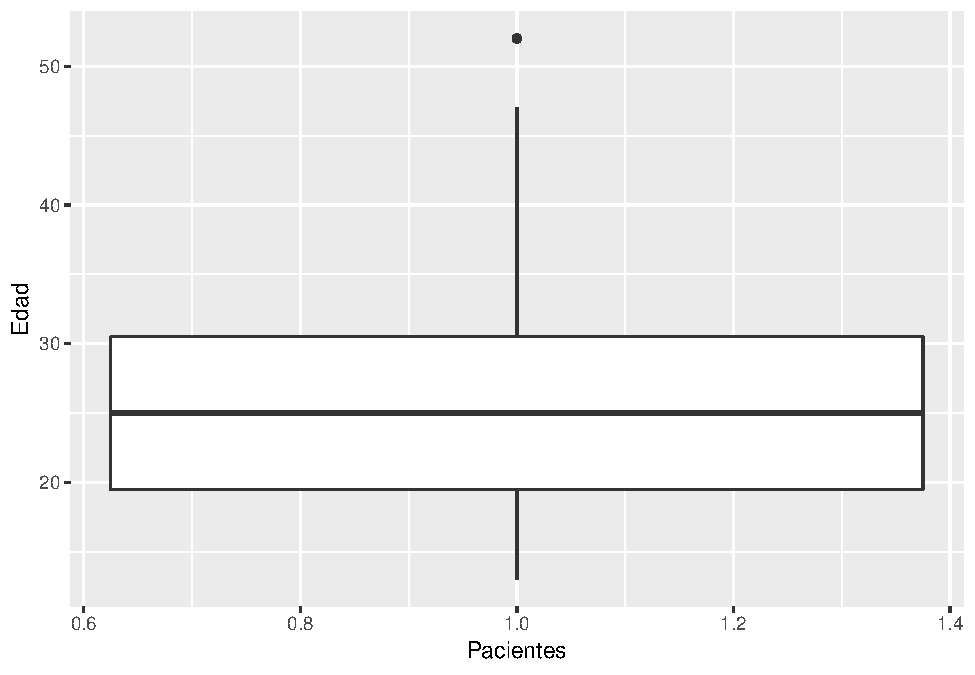
\includegraphics{codigo_files/figure-latex/grafico_estadistica_edad-1.pdf}
Pasamos el qplot a PDF:

\begin{Shaded}
\begin{Highlighting}[]
\KeywordTok{pdf}\NormalTok{(}\StringTok{"Imágenes Obtenidas/boxplotEdadPacientes.pdf"}\NormalTok{)}

\KeywordTok{qplot}\NormalTok{(}\DecValTok{1}\NormalTok{, matriz.pacientes.datos[, }\DecValTok{1}\NormalTok{], }\DataTypeTok{xlab =} \StringTok{"Pacientes"}\NormalTok{, }\DataTypeTok{ylab =} \StringTok{"Edad"}\NormalTok{, }\DataTypeTok{geom=}\StringTok{"boxplot"}\NormalTok{)}

\NormalTok{dev.off}
\end{Highlighting}
\end{Shaded}

\begin{verbatim}
## function (which = dev.cur()) 
## {
##     if (which == 1) 
##         stop("cannot shut down device 1 (the null device)")
##     .External(C_devoff, as.integer(which))
##     dev.cur()
## }
## <bytecode: 0x000000001645cb40>
## <environment: namespace:grDevices>
\end{verbatim}

Finalmente, veo un resúmen de cada columna

\begin{Shaded}
\begin{Highlighting}[]
\KeywordTok{summary}\NormalTok{(matriz.pacientes.datos)}
\end{Highlighting}
\end{Shaded}

\begin{verbatim}
##       edad            sex        rel_ctxo_rel_mala rel_ctxo_trauma 
##  Min.   :13.00   Min.   :0.000   Min.   :0.0000    Min.   :0.0000  
##  1st Qu.:19.50   1st Qu.:0.000   1st Qu.:0.0000    1st Qu.:0.0000  
##  Median :25.00   Median :0.000   Median :0.0000    Median :0.0000  
##  Mean   :26.46   Mean   :0.209   Mean   :0.1343    Mean   :0.3582  
##  3rd Qu.:30.50   3rd Qu.:0.000   3rd Qu.:0.0000    3rd Qu.:1.0000  
##  Max.   :52.00   Max.   :1.000   Max.   :1.0000    Max.   :1.0000  
##  rel_ctxo_buena      ed_perm          ed_norm          ed_estr      
##  Min.   :0.0000   Min.   :0.0000   Min.   :0.0000   Min.   :0.0000  
##  1st Qu.:0.0000   1st Qu.:0.0000   1st Qu.:0.0000   1st Qu.:0.0000  
##  Median :1.0000   Median :0.0000   Median :0.0000   Median :0.0000  
##  Mean   :0.5075   Mean   :0.2836   Mean   :0.4925   Mean   :0.2239  
##  3rd Qu.:1.0000   3rd Qu.:1.0000   3rd Qu.:1.0000   3rd Qu.:0.0000  
##  Max.   :1.0000   Max.   :1.0000   Max.   :1.0000   Max.   :1.0000  
##     resil_ba         resil_me         resil_al          pen_dic      
##  Min.   :0.0000   Min.   :0.0000   Min.   :0.00000   Min.   :0.0000  
##  1st Qu.:0.0000   1st Qu.:0.0000   1st Qu.:0.00000   1st Qu.:1.0000  
##  Median :1.0000   Median :0.0000   Median :0.00000   Median :1.0000  
##  Mean   :0.5672   Mean   :0.4179   Mean   :0.01493   Mean   :0.8955  
##  3rd Qu.:1.0000   3rd Qu.:1.0000   3rd Qu.:0.00000   3rd Qu.:1.0000  
##  Max.   :1.0000   Max.   :1.0000   Max.   :1.00000   Max.   :1.0000  
##      gen_ex            etiq           fil_men         max_min      
##  Min.   :0.0000   Min.   :0.0000   Min.   :0.000   Min.   :0.0000  
##  1st Qu.:1.0000   1st Qu.:0.5000   1st Qu.:1.000   1st Qu.:1.0000  
##  Median :1.0000   Median :1.0000   Median :1.000   Median :1.0000  
##  Mean   :0.9552   Mean   :0.7463   Mean   :0.791   Mean   :0.9701  
##  3rd Qu.:1.0000   3rd Qu.:1.0000   3rd Qu.:1.000   3rd Qu.:1.0000  
##  Max.   :1.0000   Max.   :1.0000   Max.   :1.000   Max.   :1.0000  
##     conc_arb         pseu_res           deb            raz_emo     
##  Min.   :0.0000   Min.   :0.0000   Min.   :0.0000   Min.   :0.000  
##  1st Qu.:1.0000   1st Qu.:0.0000   1st Qu.:1.0000   1st Qu.:1.000  
##  Median :1.0000   Median :1.0000   Median :1.0000   Median :1.000  
##  Mean   :0.9851   Mean   :0.5075   Mean   :0.9403   Mean   :0.791  
##  3rd Qu.:1.0000   3rd Qu.:1.0000   3rd Qu.:1.0000   3rd Qu.:1.000  
##  Max.   :1.0000   Max.   :1.0000   Max.   :1.0000   Max.   :1.000  
##      inhib            asert            agres            impuls      
##  Min.   :0.0000   Min.   :0.0000   Min.   :0.0000   Min.   :0.0000  
##  1st Qu.:0.0000   1st Qu.:0.0000   1st Qu.:0.0000   1st Qu.:0.0000  
##  Median :1.0000   Median :0.0000   Median :0.0000   Median :1.0000  
##  Mean   :0.6567   Mean   :0.1343   Mean   :0.2239   Mean   :0.6119  
##  3rd Qu.:1.0000   3rd Qu.:0.0000   3rd Qu.:0.0000   3rd Qu.:1.0000  
##  Max.   :1.0000   Max.   :1.0000   Max.   :1.0000   Max.   :1.0000
\end{verbatim}

Como se puede ver, los datos de los pacientes están muy distanciados, y
además su media es muy alta. Así, la media de la edad difiere
enormemente del resto de valores de la matriz. Debido a ello, debemos de
hacer un preprocesado de los datos del problema.

\hypertarget{preparacion-de-los-datos}{%
\section{Preparación de los datos}\label{preparacion-de-los-datos}}

Como he comentado antes, Lo que voy a hacer ahora es un centrado y
escalado de los datos de la matriz. De esta manera, la red neuronal no
tendrá ningún valor que destaque especialmente y con ello no dará de
inicio más peso a unos valores que a otros, ya que no lo buscamos.

Ahora hacemos un centrado y escalado de los datos, ya que la edad no
sigue el rango del resto de valores, y distorsionaría la predicción

\begin{Shaded}
\begin{Highlighting}[]
\NormalTok{preObjeto <-}\StringTok{ }\KeywordTok{preProcess}\NormalTok{(matriz.pacientes.datos, }\DataTypeTok{method=}\KeywordTok{c}\NormalTok{(}\StringTok{"center"}\NormalTok{, }\StringTok{"scale"}\NormalTok{))  }\CommentTok{# Quiero hacer un centrado y escalado}
\NormalTok{matriz.pacientes.datos.centscal <-}\StringTok{ }\KeywordTok{predict}\NormalTok{(preObjeto, matriz.pacientes.datos) }\CommentTok{# Obtengo los valores en la matriz centscal}
\end{Highlighting}
\end{Shaded}

Después del preprocesado, aunque con los datos no preprocesados, voy a
hacer la visualización de algunas relaciones entre variables, de tal
manera que podamos ver gráficamente algunos aspectos interesantes:

\hypertarget{visualizacion-de-datos}{%
\subsection{Visualización de Datos}\label{visualizacion-de-datos}}

Para empezar voy a sacar una nube de palabras para mostrar los nombres
más comúnes en los datos facilitados:

\begin{Shaded}
\begin{Highlighting}[]
\CommentTok{# Lo primero que tengo que hacer es contar la frecuencia de los nombres}

\NormalTok{dataNombres <-}\StringTok{ }\KeywordTok{ddply}\NormalTok{(dataset,.(nom),nrow)}
\NormalTok{dataNombres <-}\StringTok{ }\NormalTok{dataNombres[}\KeywordTok{order}\NormalTok{(dataNombres}\OperatorTok{$}\NormalTok{V1, }\DataTypeTok{decreasing =} \OtherTok{TRUE}\NormalTok{), ]}
\end{Highlighting}
\end{Shaded}

Una vez que tengo los nombres contados y ordenados, es el momento de
crear la WordCloud

\begin{Shaded}
\begin{Highlighting}[]
\KeywordTok{set.seed}\NormalTok{(}\DecValTok{9999}\NormalTok{) }\CommentTok{# Para el mantenimiento del mismo patrón}

\KeywordTok{wordcloud}\NormalTok{(}\DataTypeTok{words =}\NormalTok{ dataNombres}\OperatorTok{$}\NormalTok{nom, }\DataTypeTok{freq =}\NormalTok{ dataNombres}\OperatorTok{$}\NormalTok{V1, }\DataTypeTok{min.freq =} \DecValTok{1}\NormalTok{, }\DataTypeTok{random.order=}\OtherTok{FALSE}\NormalTok{, }\DataTypeTok{rot.per=}\FloatTok{0.5}\NormalTok{, }\DataTypeTok{colors=}\KeywordTok{c}\NormalTok{(}\StringTok{"Orange"}\NormalTok{,}\StringTok{"Purple"}\NormalTok{,}\StringTok{"Pink"}\NormalTok{, }\StringTok{"Red"}\NormalTok{, }\StringTok{"Yellow"}\NormalTok{, }\StringTok{"Green"}\NormalTok{, }\StringTok{"Blue"}\NormalTok{, }\StringTok{"Black"}\NormalTok{))}
\end{Highlighting}
\end{Shaded}

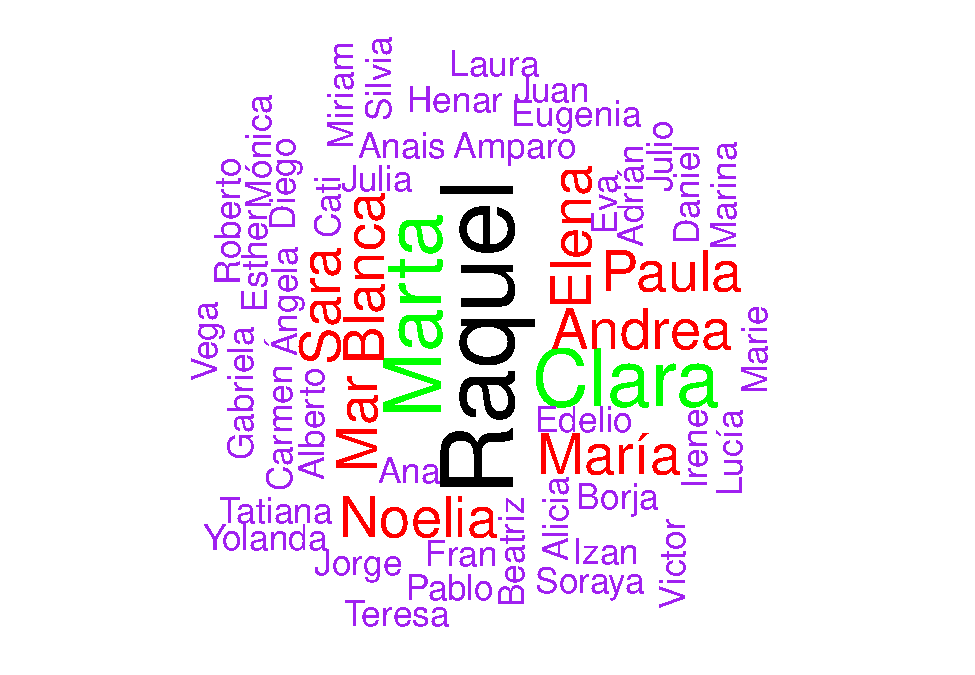
\includegraphics{codigo_files/figure-latex/wordcloud-1.pdf}

Lo pasamos a PDF:

\begin{Shaded}
\begin{Highlighting}[]
\KeywordTok{set.seed}\NormalTok{(}\DecValTok{9999}\NormalTok{)}

\KeywordTok{pdf}\NormalTok{(}\StringTok{"Imágenes Obtenidas/wordcloudNombresPacientes.pdf"}\NormalTok{)}

\KeywordTok{wordcloud}\NormalTok{(}\DataTypeTok{words =}\NormalTok{ dataNombres}\OperatorTok{$}\NormalTok{nom, }\DataTypeTok{freq =}\NormalTok{ dataNombres}\OperatorTok{$}\NormalTok{V1, }\DataTypeTok{min.freq =} \DecValTok{1}\NormalTok{, }\DataTypeTok{random.order=}\OtherTok{FALSE}\NormalTok{, }\DataTypeTok{rot.per=}\FloatTok{0.5}\NormalTok{, }\DataTypeTok{colors=}\KeywordTok{c}\NormalTok{(}\StringTok{"Orange"}\NormalTok{,}\StringTok{"Purple"}\NormalTok{,}\StringTok{"Pink"}\NormalTok{, }\StringTok{"Red"}\NormalTok{, }\StringTok{"Yellow"}\NormalTok{, }\StringTok{"Green"}\NormalTok{, }\StringTok{"Blue"}\NormalTok{, }\StringTok{"Black"}\NormalTok{))}

\NormalTok{dev.off}
\end{Highlighting}
\end{Shaded}

\begin{verbatim}
## function (which = dev.cur()) 
## {
##     if (which == 1) 
##         stop("cannot shut down device 1 (the null device)")
##     .External(C_devoff, as.integer(which))
##     dev.cur()
## }
## <bytecode: 0x000000001645cb40>
## <environment: namespace:grDevices>
\end{verbatim}

Ahora voy a sacar un plot para ver la relación entre la edad y el sexo
de las personas que están en consulta

\begin{Shaded}
\begin{Highlighting}[]
\KeywordTok{plot}\NormalTok{(matriz.pacientes.datos[,}\DecValTok{1}\NormalTok{], matriz.pacientes.datos[,}\DecValTok{2}\NormalTok{], }\DataTypeTok{xlab=}\StringTok{"Edad"}\NormalTok{, }\DataTypeTok{ylab=}\StringTok{"Sexo (0 - mujer, 1 - hombre)"}\NormalTok{, }\DataTypeTok{main=}\StringTok{"Edad & Sexo"}\NormalTok{)}
\end{Highlighting}
\end{Shaded}

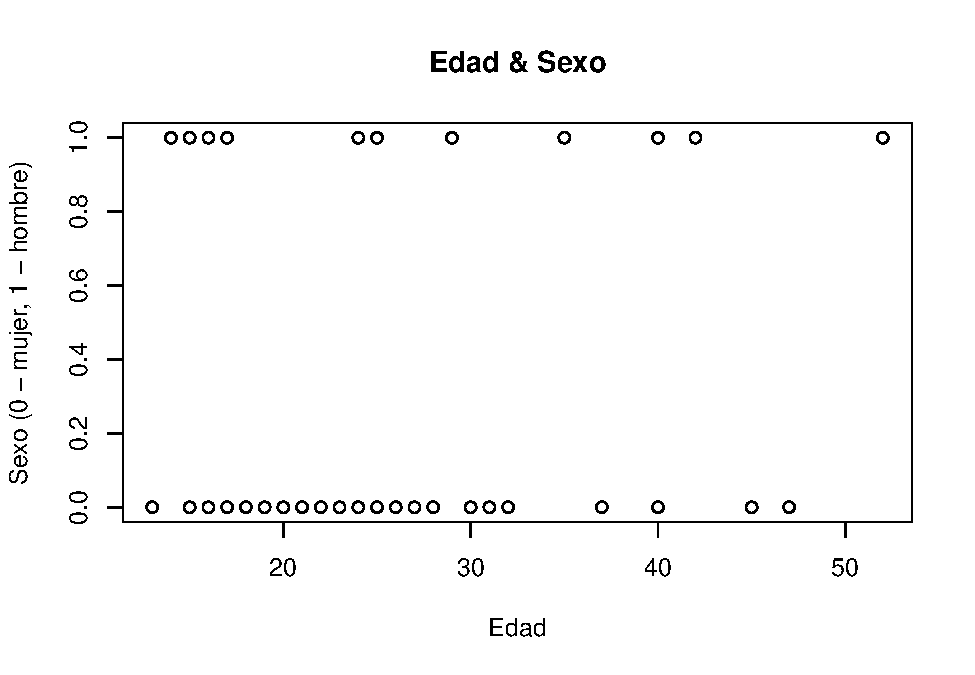
\includegraphics{codigo_files/figure-latex/grafico_edad_sexo-1.pdf}

Lo pasamos a PDF:

\begin{Shaded}
\begin{Highlighting}[]
\KeywordTok{pdf}\NormalTok{(}\StringTok{"Imágenes Obtenidas/GráficoEdad-Sexo.pdf"}\NormalTok{)}

\KeywordTok{plot}\NormalTok{(matriz.pacientes.datos[,}\DecValTok{1}\NormalTok{], matriz.pacientes.datos[,}\DecValTok{2}\NormalTok{], }\DataTypeTok{xlab=}\StringTok{"Edad"}\NormalTok{, }\DataTypeTok{ylab=}\StringTok{"Sexo (0 - mujer, 1 - hombre)"}\NormalTok{, }\DataTypeTok{main=}\StringTok{"Edad & Sexo"}\NormalTok{)}

\NormalTok{dev.off}
\end{Highlighting}
\end{Shaded}

\begin{verbatim}
## function (which = dev.cur()) 
## {
##     if (which == 1) 
##         stop("cannot shut down device 1 (the null device)")
##     .External(C_devoff, as.integer(which))
##     dev.cur()
## }
## <bytecode: 0x000000001645cb40>
## <environment: namespace:grDevices>
\end{verbatim}

Otro plot para ver la correlación entre ser agresivo y ser impulsivo

\begin{Shaded}
\begin{Highlighting}[]
\NormalTok{rf <-}\StringTok{ }\KeywordTok{colorRampPalette}\NormalTok{(}\KeywordTok{rev}\NormalTok{(}\KeywordTok{brewer.pal}\NormalTok{(}\DecValTok{4}\NormalTok{,}\StringTok{'Spectral'}\NormalTok{)))}
\NormalTok{df <-}\StringTok{ }\KeywordTok{data.frame}\NormalTok{(matriz.pacientes.datos[, }\DecValTok{23}\NormalTok{], matriz.pacientes.datos[, }\DecValTok{24}\NormalTok{])}
\NormalTok{h <-}\StringTok{ }\KeywordTok{hexbin}\NormalTok{(df)}

\KeywordTok{plot}\NormalTok{(h, }\DataTypeTok{colramp=}\NormalTok{rf, }\DataTypeTok{xlab=}\StringTok{"Agresivo"}\NormalTok{, }\DataTypeTok{ylab=}\StringTok{"Impulsivo"}\NormalTok{, }\DataTypeTok{main=}\StringTok{"Agresivo Vs Impulsivo"}\NormalTok{)}
\end{Highlighting}
\end{Shaded}

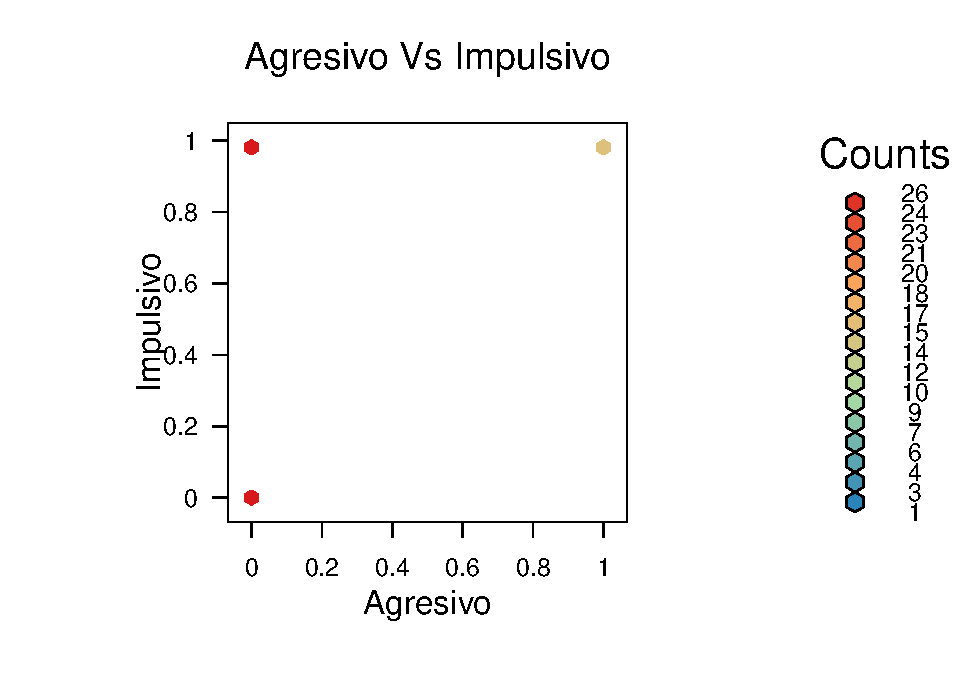
\includegraphics{codigo_files/figure-latex/grafico_agresivo_impulsivo-1.pdf}

Lo pasamos a PDF:

\begin{Shaded}
\begin{Highlighting}[]
\KeywordTok{pdf}\NormalTok{(}\StringTok{"Imágenes Obtenidas/GraficoAgresivoVsImpulsivo.pdf"}\NormalTok{)}

\KeywordTok{plot}\NormalTok{(h, }\DataTypeTok{colramp=}\NormalTok{rf, }\DataTypeTok{xlab=}\StringTok{"Agresivo"}\NormalTok{, }\DataTypeTok{ylab=}\StringTok{"Impulsivo"}\NormalTok{, }\DataTypeTok{main=}\StringTok{"Agresivo Vs Impulsivo"}\NormalTok{)}

\NormalTok{dev.off}
\end{Highlighting}
\end{Shaded}

\begin{verbatim}
## function (which = dev.cur()) 
## {
##     if (which == 1) 
##         stop("cannot shut down device 1 (the null device)")
##     .External(C_devoff, as.integer(which))
##     dev.cur()
## }
## <bytecode: 0x000000001645cb40>
## <environment: namespace:grDevices>
\end{verbatim}

Otro plot similar para ver la relación de ser inhibido e impulsivo

\begin{Shaded}
\begin{Highlighting}[]
\NormalTok{df <-}\StringTok{ }\KeywordTok{data.frame}\NormalTok{(matriz.pacientes.datos[, }\DecValTok{21}\NormalTok{], matriz.pacientes.datos[, }\DecValTok{24}\NormalTok{])}
\NormalTok{h <-}\StringTok{ }\KeywordTok{hexbin}\NormalTok{(df)}

\KeywordTok{plot}\NormalTok{(h, }\DataTypeTok{colramp=}\NormalTok{rf, }\DataTypeTok{xlab=}\StringTok{"Inhibido"}\NormalTok{, }\DataTypeTok{ylab=}\StringTok{"Impulsivo"}\NormalTok{, }\DataTypeTok{main=}\StringTok{"Inhibido Vs Impulsivo"}\NormalTok{)}
\end{Highlighting}
\end{Shaded}

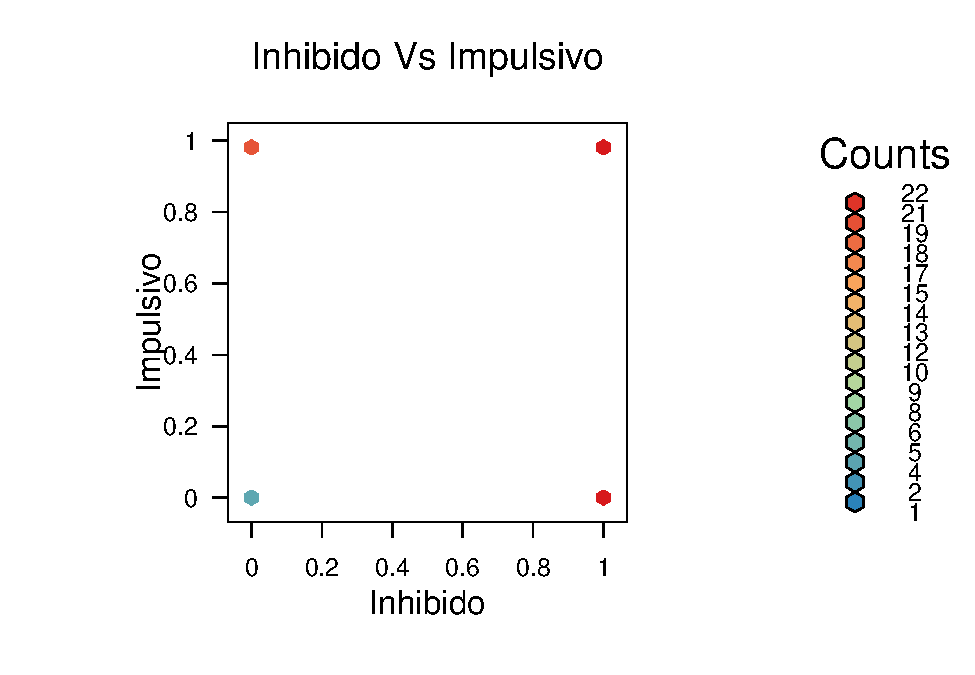
\includegraphics{codigo_files/figure-latex/grafico_inhibido_impulsivo-1.pdf}

Lo guardo en PDF:

\begin{Shaded}
\begin{Highlighting}[]
\KeywordTok{pdf}\NormalTok{(}\StringTok{"Imágenes Obtenidas/GraficoInhibidoVsImpulsivo.pdf"}\NormalTok{)}

\KeywordTok{plot}\NormalTok{(h, }\DataTypeTok{colramp=}\NormalTok{rf, }\DataTypeTok{xlab=}\StringTok{"Inhibido"}\NormalTok{, }\DataTypeTok{ylab=}\StringTok{"Impulsivo"}\NormalTok{, }\DataTypeTok{main=}\StringTok{"Inhibido Vs Impulsivo"}\NormalTok{)}

\NormalTok{dev.off}
\end{Highlighting}
\end{Shaded}

\begin{verbatim}
## function (which = dev.cur()) 
## {
##     if (which == 1) 
##         stop("cannot shut down device 1 (the null device)")
##     .External(C_devoff, as.integer(which))
##     dev.cur()
## }
## <bytecode: 0x000000001645cb40>
## <environment: namespace:grDevices>
\end{verbatim}

Voy a ver la relación entre el razonamiento emocional (actuar según tus
sentimientos) y la impulsividad

\begin{Shaded}
\begin{Highlighting}[]
\NormalTok{df <-}\StringTok{ }\KeywordTok{data.frame}\NormalTok{(matriz.pacientes.datos[, }\DecValTok{20}\NormalTok{], matriz.pacientes.datos[, }\DecValTok{24}\NormalTok{])}
\NormalTok{h <-}\StringTok{ }\KeywordTok{hexbin}\NormalTok{(df)}

\KeywordTok{plot}\NormalTok{(h, }\DataTypeTok{colramp=}\NormalTok{rf, }\DataTypeTok{xlab=}\StringTok{"Razonamiento Emocional"}\NormalTok{, }\DataTypeTok{ylab=}\StringTok{"Impulsivo"}\NormalTok{, }\DataTypeTok{main=}\StringTok{"Razonamiento Emocional Vs Impulsivo"}\NormalTok{)}
\end{Highlighting}
\end{Shaded}

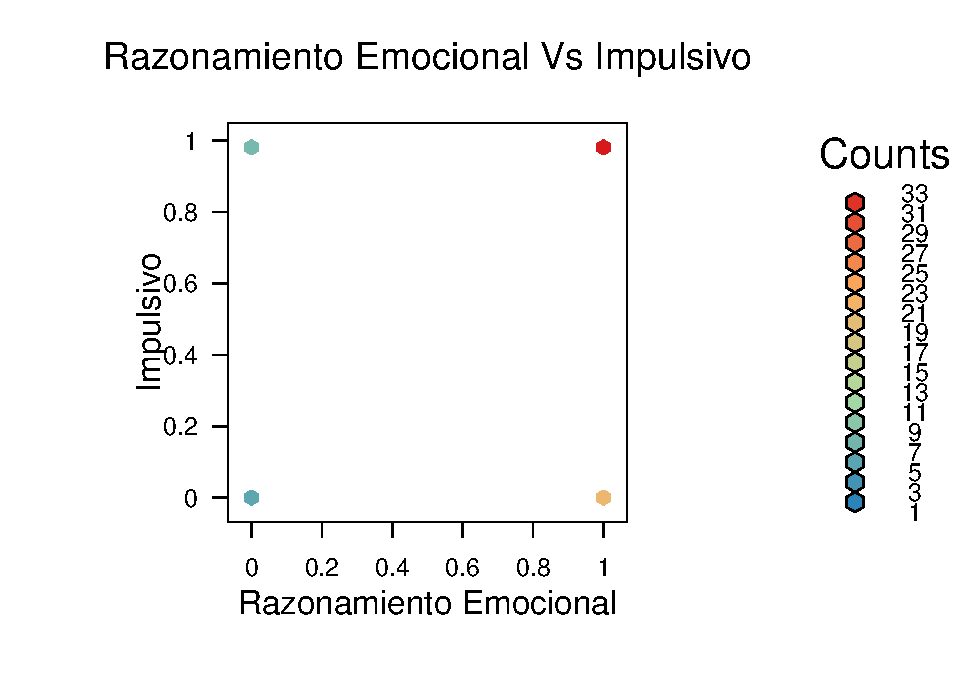
\includegraphics{codigo_files/figure-latex/grafico_razEm_Impulsivo-1.pdf}

Lo guardo en PDF:

\begin{Shaded}
\begin{Highlighting}[]
\KeywordTok{pdf}\NormalTok{(}\StringTok{"Imágenes Obtenidas/GraficoRazonamientoEmocionalVsImpulsivo.pdf"}\NormalTok{)}

\KeywordTok{plot}\NormalTok{(h, }\DataTypeTok{colramp=}\NormalTok{rf, }\DataTypeTok{xlab=}\StringTok{"Razonamiento Emocional"}\NormalTok{, }\DataTypeTok{ylab=}\StringTok{"Impulsivo"}\NormalTok{, }\DataTypeTok{main=}\StringTok{"Razonamiento Emocional Vs Impulsivo"}\NormalTok{)}

\NormalTok{dev.off}
\end{Highlighting}
\end{Shaded}

\begin{verbatim}
## function (which = dev.cur()) 
## {
##     if (which == 1) 
##         stop("cannot shut down device 1 (the null device)")
##     .External(C_devoff, as.integer(which))
##     dev.cur()
## }
## <bytecode: 0x000000001645cb40>
## <environment: namespace:grDevices>
\end{verbatim}

Ahora quiero sacar una relación entre ser agresivo y ver el grupo en el
que están

\begin{Shaded}
\begin{Highlighting}[]
\NormalTok{rf <-}\StringTok{ }\KeywordTok{colorRampPalette}\NormalTok{(}\KeywordTok{rev}\NormalTok{(}\KeywordTok{brewer.pal}\NormalTok{(}\DecValTok{4}\NormalTok{,}\StringTok{'Spectral'}\NormalTok{)))}
\NormalTok{df <-}\StringTok{ }\KeywordTok{data.frame}\NormalTok{(matriz.pacientes.datos[, }\DecValTok{23}\NormalTok{], matriz.pacientes.etiquetas[, }\DecValTok{25}\NormalTok{])}
\NormalTok{h <-}\StringTok{ }\KeywordTok{hexbin}\NormalTok{(df)}

\KeywordTok{plot}\NormalTok{(h, }\DataTypeTok{colramp=}\NormalTok{rf, }\DataTypeTok{xlab=}\StringTok{"Agresivo"}\NormalTok{, }\DataTypeTok{ylab=}\StringTok{"Grupo"}\NormalTok{, }\DataTypeTok{main=}\StringTok{"Agresivo Y Grupo Real"}\NormalTok{)}
\end{Highlighting}
\end{Shaded}

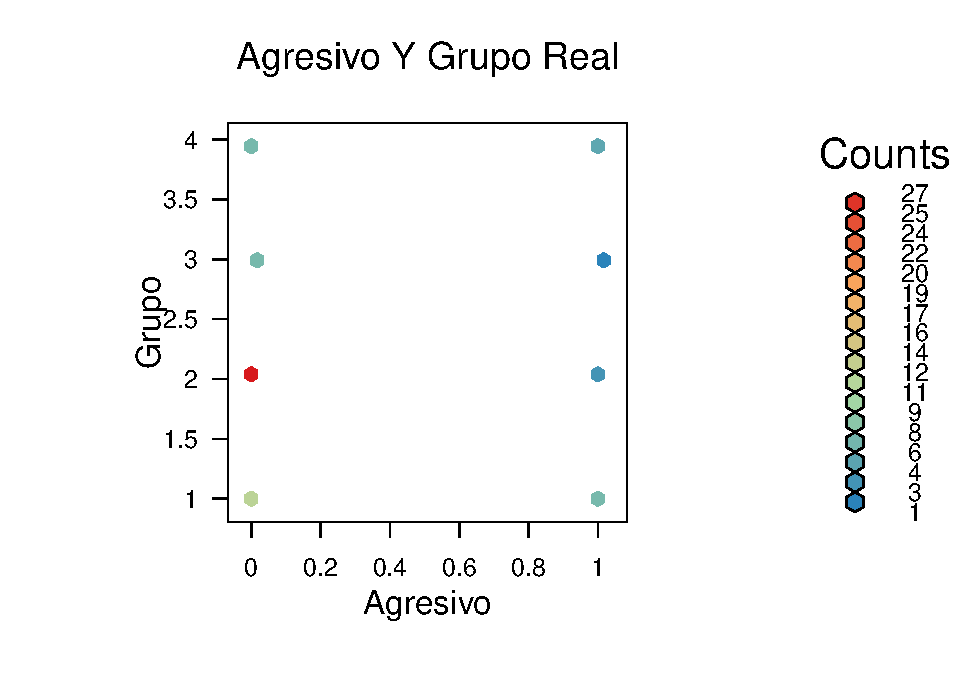
\includegraphics{codigo_files/figure-latex/grafico_agresivo_grupo-1.pdf}

Lo guardo en PDF:

\begin{Shaded}
\begin{Highlighting}[]
\KeywordTok{pdf}\NormalTok{(}\StringTok{"Imágenes Obtenidas/GraficoAgresivoVsGrupo.pdf"}\NormalTok{)}

\KeywordTok{plot}\NormalTok{(h, }\DataTypeTok{colramp=}\NormalTok{rf, }\DataTypeTok{xlab=}\StringTok{"Agresivo"}\NormalTok{, }\DataTypeTok{ylab=}\StringTok{"Grupo"}\NormalTok{, }\DataTypeTok{main=}\StringTok{"Agresivo Y Grupo Real"}\NormalTok{)}

\NormalTok{dev.off}
\end{Highlighting}
\end{Shaded}

\begin{verbatim}
## function (which = dev.cur()) 
## {
##     if (which == 1) 
##         stop("cannot shut down device 1 (the null device)")
##     .External(C_devoff, as.integer(which))
##     dev.cur()
## }
## <bytecode: 0x000000001645cb40>
## <environment: namespace:grDevices>
\end{verbatim}

Voy a hacer lo mismo con la impulsividad

\begin{Shaded}
\begin{Highlighting}[]
\NormalTok{rf <-}\StringTok{ }\KeywordTok{colorRampPalette}\NormalTok{(}\KeywordTok{rev}\NormalTok{(}\KeywordTok{brewer.pal}\NormalTok{(}\DecValTok{4}\NormalTok{,}\StringTok{'Spectral'}\NormalTok{)))}
\NormalTok{df <-}\StringTok{ }\KeywordTok{data.frame}\NormalTok{(matriz.pacientes.datos[, }\DecValTok{24}\NormalTok{], matriz.pacientes.etiquetas[, }\DecValTok{25}\NormalTok{])}
\NormalTok{h <-}\StringTok{ }\KeywordTok{hexbin}\NormalTok{(df)}

\KeywordTok{plot}\NormalTok{(h, }\DataTypeTok{colramp=}\NormalTok{rf, }\DataTypeTok{xlab=}\StringTok{"Impulsivo"}\NormalTok{, }\DataTypeTok{ylab=}\StringTok{"Grupo"}\NormalTok{, }\DataTypeTok{main=}\StringTok{"Impulsivo y Grupo Real"}\NormalTok{)}
\end{Highlighting}
\end{Shaded}

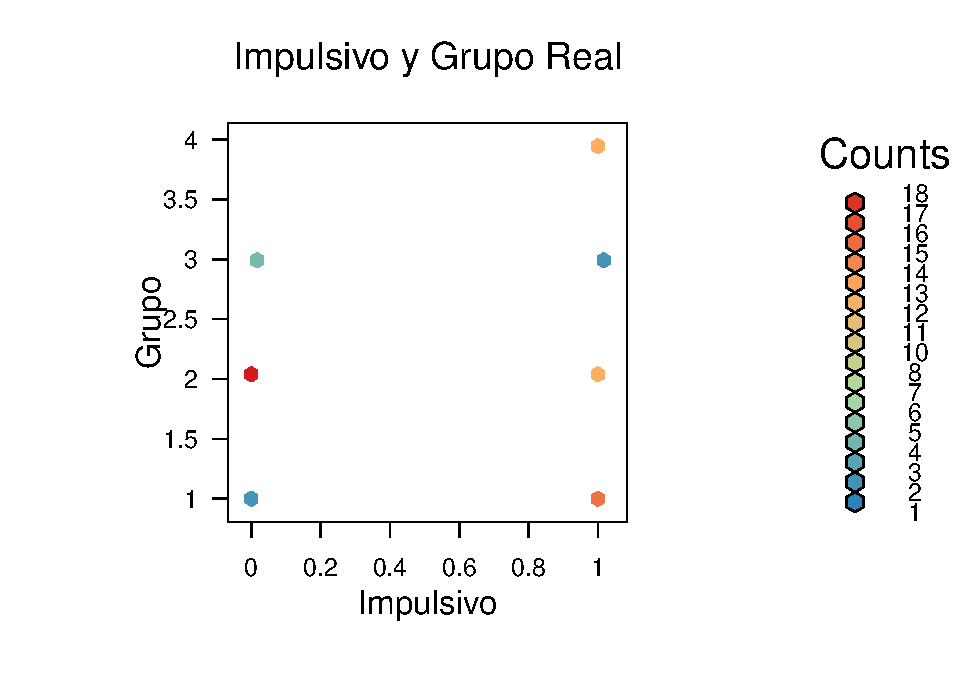
\includegraphics{codigo_files/figure-latex/grafico_impulsivo_grupo-1.pdf}

Lo guardo en PDF:

\begin{Shaded}
\begin{Highlighting}[]
\KeywordTok{pdf}\NormalTok{(}\StringTok{"Imágenes Obtenidas/GraficoImpulsivoVsGrupo.pdf"}\NormalTok{)}

\KeywordTok{plot}\NormalTok{(h, }\DataTypeTok{colramp=}\NormalTok{rf, }\DataTypeTok{xlab=}\StringTok{"Impulsivo"}\NormalTok{, }\DataTypeTok{ylab=}\StringTok{"Grupo"}\NormalTok{, }\DataTypeTok{main=}\StringTok{"Impulsivo y Grupo Real"}\NormalTok{)}

\NormalTok{dev.off}
\end{Highlighting}
\end{Shaded}

\begin{verbatim}
## function (which = dev.cur()) 
## {
##     if (which == 1) 
##         stop("cannot shut down device 1 (the null device)")
##     .External(C_devoff, as.integer(which))
##     dev.cur()
## }
## <bytecode: 0x000000001645cb40>
## <environment: namespace:grDevices>
\end{verbatim}

De estas gráficas estamos obteniendo información realmente interesante
antes de la predicción de los datos. He preferido hacer gráficas en 2D
porque las gráficas en 3D son mucho más difíciles de interpretar que
estas bonitas gráficas en 2D

Vamos a ver la correlación que tienen mis variables

\begin{Shaded}
\begin{Highlighting}[]
\NormalTok{res <-}\StringTok{ }\KeywordTok{cor}\NormalTok{(matriz.pacientes.datos[, }\DecValTok{1}\OperatorTok{:}\DecValTok{24}\NormalTok{], }\DataTypeTok{method =} \StringTok{"spearman"}\NormalTok{) }\CommentTok{# Por mi tipo de datos, hacemos la correlación por spearman}
\KeywordTok{options}\NormalTok{(}\DataTypeTok{width =} \DecValTok{100}\NormalTok{)}
\NormalTok{res.round <-}\StringTok{ }\KeywordTok{round}\NormalTok{(res, }\DecValTok{2}\NormalTok{)}
\end{Highlighting}
\end{Shaded}

Como saca una tabla enorme, lo que voy a hacer es usar una librería que
me da una función para sacar de una forma bonita las correlaciones entre
las variables.

\begin{Shaded}
\begin{Highlighting}[]
\KeywordTok{corrplot}\NormalTok{(res.round, }\DataTypeTok{method=}\StringTok{"circle"}\NormalTok{)}
\end{Highlighting}
\end{Shaded}

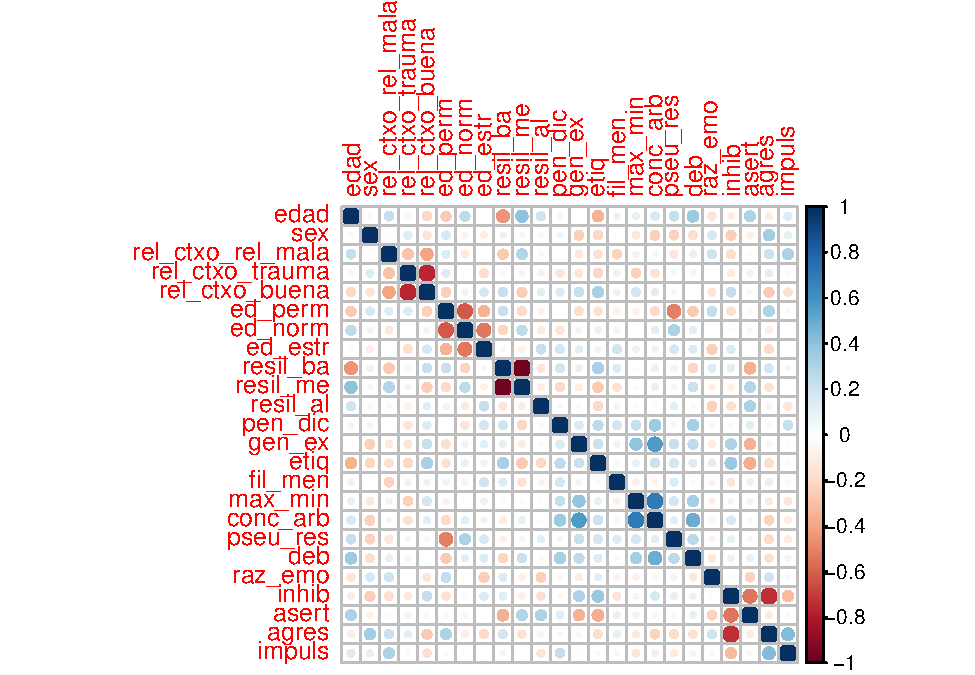
\includegraphics{codigo_files/figure-latex/grafico_correlaciones_variables-1.pdf}

Guardamos la matriz de correlación en PDF para tener mejor
visualización:

\begin{Shaded}
\begin{Highlighting}[]
\KeywordTok{pdf}\NormalTok{(}\StringTok{"Imágenes Obtenidas/Corrplot.pdf"}\NormalTok{)}

\KeywordTok{corrplot}\NormalTok{(res.round, }\DataTypeTok{method=}\StringTok{"circle"}\NormalTok{)}

\NormalTok{dev.off}
\end{Highlighting}
\end{Shaded}

\begin{verbatim}
## function (which = dev.cur()) 
## {
##     if (which == 1) 
##         stop("cannot shut down device 1 (the null device)")
##     .External(C_devoff, as.integer(which))
##     dev.cur()
## }
## <bytecode: 0x000000001645cb40>
## <environment: namespace:grDevices>
\end{verbatim}

Como podemos ver, por ejemplo, resiliencia baja y media tienen una
correlación de -1, ya que si hay una no hay la otra y viceversa. Esto
pasa igual con las relaciones entre contexto, ya que buena - trauma,
trauma - mala, mala - buena tienen que ser inversas.

Ahora voy a sacar un PCA para ver la importancia de las variables:

Para los cálculos, uso la matriz con el centrado y escalado ya hechos

\begin{Shaded}
\begin{Highlighting}[]
\NormalTok{resultado.pca <-}\StringTok{ }\KeywordTok{PCA}\NormalTok{(matriz.pacientes.datos.centscal, }\DataTypeTok{graph =} \OtherTok{FALSE}\NormalTok{)}

\CommentTok{#Con la siguiente línea podemos ver que podemos hacer con esto calculado}
\KeywordTok{print}\NormalTok{(resultado.pca)}
\end{Highlighting}
\end{Shaded}

\begin{verbatim}
## **Results for the Principal Component Analysis (PCA)**
## The analysis was performed on 67 individuals, described by 24 variables
## *The results are available in the following objects:
## 
##    name               description                          
## 1  "$eig"             "eigenvalues"                        
## 2  "$var"             "results for the variables"          
## 3  "$var$coord"       "coord. for the variables"           
## 4  "$var$cor"         "correlations variables - dimensions"
## 5  "$var$cos2"        "cos2 for the variables"             
## 6  "$var$contrib"     "contributions of the variables"     
## 7  "$ind"             "results for the individuals"        
## 8  "$ind$coord"       "coord. for the individuals"         
## 9  "$ind$cos2"        "cos2 for the individuals"           
## 10 "$ind$contrib"     "contributions of the individuals"   
## 11 "$call"            "summary statistics"                 
## 12 "$call$centre"     "mean of the variables"              
## 13 "$call$ecart.type" "standard error of the variables"    
## 14 "$call$row.w"      "weights for the individuals"        
## 15 "$call$col.w"      "weights for the variables"
\end{verbatim}

Nos interesa ver los eigenvalues, que son los que presentarán la
cantidad de varianza que aportan las variables:

\begin{Shaded}
\begin{Highlighting}[]
\NormalTok{eigenvalues.PCA <-}\StringTok{ }\NormalTok{resultado.pca}\OperatorTok{$}\NormalTok{eig}
\NormalTok{eigenvalues.PCA}
\end{Highlighting}
\end{Shaded}

\begin{verbatim}
##           eigenvalue percentage of variance cumulative percentage of variance
## comp 1  3.901309e+00           1.625546e+01                          16.25546
## comp 2  3.351564e+00           1.396485e+01                          30.22031
## comp 3  2.227420e+00           9.280918e+00                          39.50122
## comp 4  2.057473e+00           8.572804e+00                          48.07403
## comp 5  1.723129e+00           7.179706e+00                          55.25373
## comp 6  1.523874e+00           6.349473e+00                          61.60321
## comp 7  1.367911e+00           5.699627e+00                          67.30283
## comp 8  1.080649e+00           4.502703e+00                          71.80554
## comp 9  9.451881e-01           3.938284e+00                          75.74382
## comp 10 9.303616e-01           3.876507e+00                          79.62033
## comp 11 8.797962e-01           3.665817e+00                          83.28615
## comp 12 8.090124e-01           3.370885e+00                          86.65703
## comp 13 6.586878e-01           2.744533e+00                          89.40156
## comp 14 6.005323e-01           2.502218e+00                          91.90378
## comp 15 4.700232e-01           1.958430e+00                          93.86221
## comp 16 4.612585e-01           1.921910e+00                          95.78412
## comp 17 3.888962e-01           1.620401e+00                          97.40452
## comp 18 2.333650e-01           9.723542e-01                          98.37688
## comp 19 2.209107e-01           9.204610e-01                          99.29734
## comp 20 1.481544e-01           6.173101e-01                          99.91465
## comp 21 2.048464e-02           8.535265e-02                         100.00000
## comp 22 1.760166e-31           7.334027e-31                         100.00000
## comp 23 7.908215e-32           3.295090e-31                         100.00000
## comp 24 7.613437e-33           3.172266e-32                         100.00000
\end{verbatim}

Como se puede comprobar, de las 24 variables (componentes) que tenemos,
la mitad de la varianza la conseguimos con aproximadamente 5 variables.
También se puede ver que a parti de las 17 variables prácticamente no
hay un aumento de la varianza. En el caso de un problema grande, sería
interesante la eliminación de algunas de las variables, para dejar un
dataset más pequeño con el que poder trabajar. En nuestro caso, nuestro
problema es pequeño, y además las variables están escogidas a mano, por
lo que no haré una reducción del dataset.

Ahora, para completar este apartado de PCA, lo que voy a hacer es sacar
la gráfica de la varianza acumulada con los valores anteriores:

\begin{Shaded}
\begin{Highlighting}[]
\NormalTok{plotPCA <-}\StringTok{ }\KeywordTok{fviz_screeplot}\NormalTok{(resultado.pca, }\DataTypeTok{ncp=}\DecValTok{24}\NormalTok{)}
\KeywordTok{plot}\NormalTok{(plotPCA)}
\end{Highlighting}
\end{Shaded}

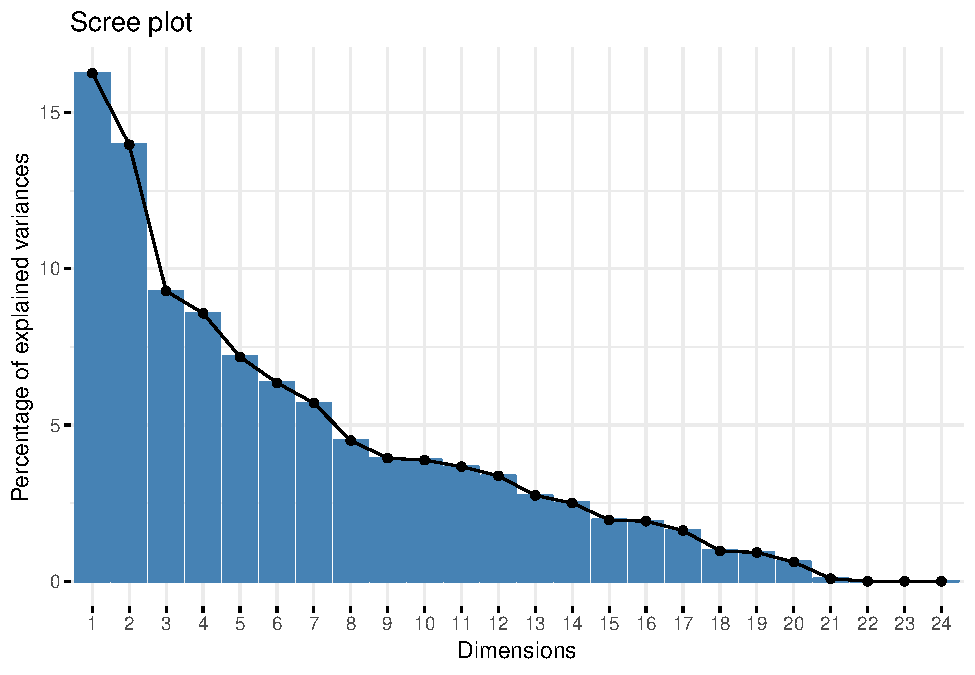
\includegraphics{codigo_files/figure-latex/PCA_eigenvalues_graph-1.pdf}

\begin{Shaded}
\begin{Highlighting}[]
\KeywordTok{fviz_pca_biplot}\NormalTok{(resultado.pca, }\DataTypeTok{repel =} \OtherTok{TRUE}\NormalTok{,}
                    \DataTypeTok{col.var =} \StringTok{"#FF0040"}\NormalTok{, }\CommentTok{# Color de las variables (vectores)}
                    \DataTypeTok{col.ind =} \StringTok{"#21610B"}\NormalTok{, }\CommentTok{# Color de cada individuo (puntos)}
                    \DataTypeTok{label =} \StringTok{"var"}\NormalTok{,}
                    \DataTypeTok{title =} \StringTok{"Plot Binario - Elementos / Dimensiones"}\NormalTok{,}
                    \DataTypeTok{geom.ind =} \StringTok{"point"}\NormalTok{,}
                    \DataTypeTok{pointshape =} \DecValTok{4}\NormalTok{)  }
\end{Highlighting}
\end{Shaded}

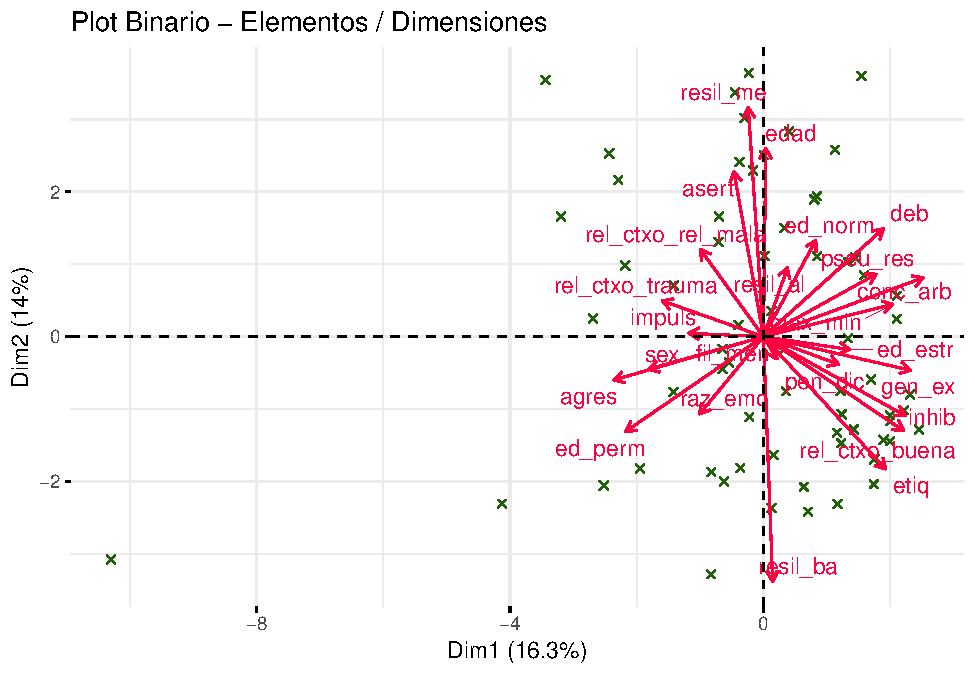
\includegraphics{codigo_files/figure-latex/PCA_eigenvalues_graph-2.pdf}

\begin{Shaded}
\begin{Highlighting}[]
\KeywordTok{ggbiplot}\NormalTok{(resultado.pca, }\DataTypeTok{ellipse=}\OtherTok{TRUE}\NormalTok{, }\DataTypeTok{labels=}\KeywordTok{rownames}\NormalTok{(dataset), }\DataTypeTok{groups=}\NormalTok{dataset}\OperatorTok{$}\NormalTok{grupo)}
\end{Highlighting}
\end{Shaded}

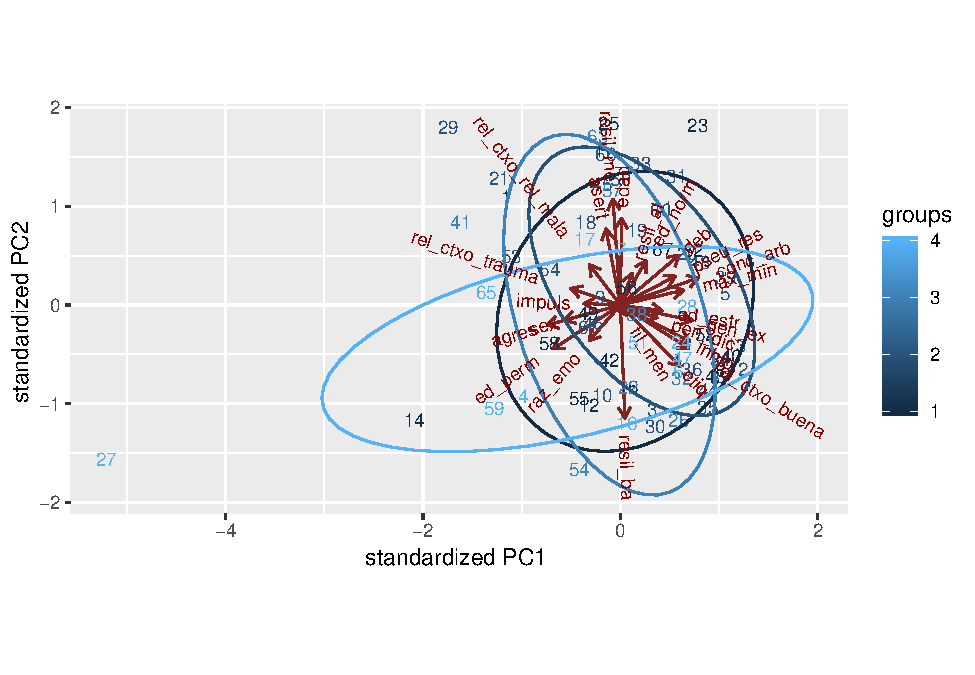
\includegraphics{codigo_files/figure-latex/PCA_eigenvalues_graph-3.pdf}

Con esto puedo sacar conclusiones al igual que con el gran gráfico de
correlaciones de variables, solo que esta representación está
intencionada para más de 2 dimensiones.

Puedo ver algunas de las conclusiones fáciles que saqué anteriormente,
como que resiliencia media es contraria a baja, o que la relación con el
contexto de trauma y mala son contrarias a buena.

Otras relaciones también puedo ver, como que los deberías y el
razonamiento emocional parecen ser ciertamente contrarios, o que el
filtro mental no depende de prácticamente nada ya que está en todo el
centro.

También es importante ver como, mediante dos componentes principales
(dos dimensiones), solo estoy explicando un del 30,2\% del total, lo que
es muy poco. Por unirlo con los gráficos anteriores, estas dos
componentes que se han elegido como x e y son las dos variables que más
varianza (y por lo tanto, explicación) tenían en el gráfico de barras
anterior.

Obtengo estos gráficos en PDF para tener una mejor visualización:

\begin{Shaded}
\begin{Highlighting}[]
\KeywordTok{pdf}\NormalTok{(}\StringTok{"Imágenes Obtenidas/GraficoEigenvalues.pdf"}\NormalTok{)}

\KeywordTok{plot}\NormalTok{(plotPCA)}

\KeywordTok{fviz_pca_biplot}\NormalTok{(resultado.pca, }\DataTypeTok{repel =} \OtherTok{TRUE}\NormalTok{,}
                    \DataTypeTok{col.var =} \StringTok{"#FF0040"}\NormalTok{, }\CommentTok{# Color de las variables (vectores)}
                    \DataTypeTok{col.ind =} \StringTok{"#21610B"}\NormalTok{, }\CommentTok{# Color de cada individuo (puntos)}
                    \DataTypeTok{label =} \StringTok{"var"}\NormalTok{,}
                    \DataTypeTok{title =} \StringTok{"Plot Binario - Elementos / Dimensiones"}\NormalTok{,}
                    \DataTypeTok{geom.ind =} \StringTok{"point"}\NormalTok{,}
                    \DataTypeTok{pointshape =} \DecValTok{4}\NormalTok{)  }

\KeywordTok{ggbiplot}\NormalTok{(resultado.pca, }\DataTypeTok{ellipse=}\OtherTok{TRUE}\NormalTok{, }\DataTypeTok{labels=}\KeywordTok{rownames}\NormalTok{(dataset), }\DataTypeTok{groups=}\NormalTok{dataset}\OperatorTok{$}\NormalTok{grupo)}

\NormalTok{dev.off}
\end{Highlighting}
\end{Shaded}

\begin{verbatim}
## function (which = dev.cur()) 
## {
##     if (which == 1) 
##         stop("cannot shut down device 1 (the null device)")
##     .External(C_devoff, as.integer(which))
##     dev.cur()
## }
## <bytecode: 0x000000001645cb40>
## <environment: namespace:grDevices>
\end{verbatim}

Ahora voy a sacar un ``Factor Map'' de las variables. Esto lo puedo
hacer gracias a las coordenadas que me da una de las variables tras
hacer el PCA. Así, voy primero a ver la tabla y luego voy a sacar el
mapa:

\begin{Shaded}
\begin{Highlighting}[]
\NormalTok{resultado.pca}\OperatorTok{$}\NormalTok{var}\OperatorTok{$}\NormalTok{coord}
\end{Highlighting}
\end{Shaded}

\begin{verbatim}
##                          Dim.1       Dim.2      Dim.3       Dim.4        Dim.5
## edad               0.009449477  0.66220660  0.2012166 -0.01688598  0.034353130
## sex               -0.461817396 -0.11469866  0.1142057  0.04821226  0.138691683
## rel_ctxo_rel_mala -0.253565155  0.30698270  0.2523704  0.54165055 -0.331171378
## rel_ctxo_trauma   -0.406566127  0.12583417 -0.2367909 -0.10989250  0.353071033
## rel_ctxo_buena     0.562872310 -0.33007031  0.0549572 -0.26405906 -0.112727268
## ed_perm           -0.553298015 -0.33359344  0.2204075  0.17649166 -0.382130027
## ed_norm            0.210631011  0.33868151 -0.4992287  0.16199773  0.581029158
## ed_estr            0.345664380 -0.04548281  0.3604255 -0.38513556 -0.283661513
## resil_ba           0.036989747 -0.86064157  0.1925883 -0.06725075  0.209126794
## resil_me          -0.060865419  0.80506164 -0.2729037  0.19505694 -0.175488418
## resil_al           0.096429585  0.24207008  0.3231128 -0.51861611 -0.140713832
## pen_dic            0.301692791 -0.09722286  0.6037969  0.09908508  0.162269610
## gen_ex             0.590510842 -0.11826460  0.1414008  0.27533229  0.139625847
## etiq               0.490832373 -0.46558987 -0.1291992  0.20553979  0.163608829
## fil_men            0.054242913 -0.07841106  0.2818291 -0.38746594  0.409914887
## max_min            0.519764910  0.11369217  0.3655504  0.32864289 -0.062767279
## conc_arb           0.641299587  0.20703282  0.2929369  0.43016356  0.005040268
## pseu_res           0.452663235  0.21985405 -0.1133463 -0.14273197  0.451008261
## deb                0.481970404  0.37956964  0.2376543  0.24593023  0.104409060
## raz_emo           -0.256501489 -0.27198444 -0.1469739  0.45651306  0.026547345
## inhib              0.569860339 -0.27821097 -0.4926674  0.08127591 -0.330837919
## asert             -0.118639889  0.57971021  0.2835803 -0.39517909  0.016646777
## agres             -0.600724015 -0.15246890  0.3900381  0.22510662  0.384194829
## impuls            -0.299148404  0.01187884  0.3756371  0.29777080  0.283406252
\end{verbatim}

Como se puede ver, me está poniendo mis 24 variables en 5 dimensiones,
con unas coordenadas concretas. Ahora, lo que voy a hacer, es
representarlo. Con esta representación podré sacar algunas conclusiones:

Ahora mi siguiente paso es sacar un gráfico de los individuos, para ver
donde están colocados en este sistema:

\begin{Shaded}
\begin{Highlighting}[]
\KeywordTok{head}\NormalTok{(resultado.pca}\OperatorTok{$}\NormalTok{ind}\OperatorTok{$}\NormalTok{coord) }\CommentTok{# Solo saco los primeros para no ocupar demasiado espacio}
\end{Highlighting}
\end{Shaded}

\begin{verbatim}
##        Dim.1      Dim.2       Dim.3      Dim.4      Dim.5
## 1 -2.2940308  2.1634024 -0.75784032  2.6256358 -0.8316371
## 2  2.4550347 -1.2849670  0.05998261 -1.1988926 -1.4255692
## 3  0.6380076 -2.0755240 -0.22249577  0.6948728 -2.1789437
## 4 -1.9455134 -1.8228537  1.57190908  0.9311446  0.9776417
## 5  2.1050031  0.2444206 -0.28941341 -0.7153514 -1.1887786
## 6  1.1614700 -1.3278368 -0.71761135  1.0750939 -0.2075874
\end{verbatim}

Ahora, tras ver que todos mis individuos tienen unas ciertas
coordenadas, vamos a representarlos gráficamente:

\begin{Shaded}
\begin{Highlighting}[]
\CommentTok{# Saco este gráfico para ver los individuos de una forma más clara}

\KeywordTok{fviz_pca_ind}\NormalTok{(resultado.pca, }\DataTypeTok{repel =}\NormalTok{ T)}
\end{Highlighting}
\end{Shaded}

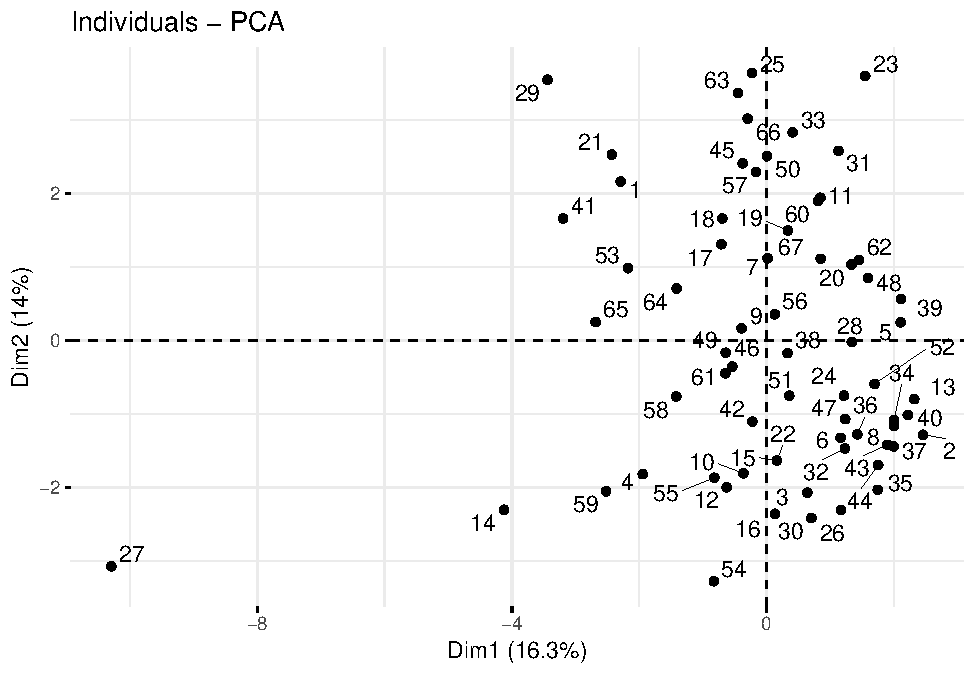
\includegraphics{codigo_files/figure-latex/plot_coordendas_individuos-1.pdf}

Exporto a PDF las coordenadas de los individuos:

\begin{Shaded}
\begin{Highlighting}[]
\KeywordTok{pdf}\NormalTok{(}\StringTok{"Imágenes Obtenidas/GraficoIndividuosPCA.pdf"}\NormalTok{)}

\KeywordTok{fviz_pca_ind}\NormalTok{(resultado.pca, }\DataTypeTok{repel =}\NormalTok{ T)}

\NormalTok{dev.off}
\end{Highlighting}
\end{Shaded}

\begin{verbatim}
## function (which = dev.cur()) 
## {
##     if (which == 1) 
##         stop("cannot shut down device 1 (the null device)")
##     .External(C_devoff, as.integer(which))
##     dev.cur()
## }
## <bytecode: 0x000000001645cb40>
## <environment: namespace:grDevices>
\end{verbatim}

Se puede ver que la mayoría de los pacientes están en torno al centro,
mientras que tenemos un outlayer, que es el número 27.

\begin{center}\rule{0.5\linewidth}{\linethickness}\end{center}

\hypertarget{modelos-de-inteligencia-artificial-supervisados}{%
\section{Modelos de Inteligencia Artificial
supervisados}\label{modelos-de-inteligencia-artificial-supervisados}}

Ahora lo que hago es coger un conjunto muy grande de los datos para
hacer el entrenamiento

\begin{Shaded}
\begin{Highlighting}[]
\NormalTok{conjuntoEntrenamiento <-}\StringTok{ }\KeywordTok{sample}\NormalTok{(}\DecValTok{1}\OperatorTok{:}\DecValTok{67}\NormalTok{, }\DecValTok{55}\NormalTok{)}
\end{Highlighting}
\end{Shaded}

1 NEURONA

Lo que voy a hacer ahora es entrenar la red neuronal con diferente
cantidad de neuronas,y voy a ir comparando el resultado\ldots{}

SIN SOFTMAX

\begin{Shaded}
\begin{Highlighting}[]
\KeywordTok{set.seed}\NormalTok{(}\DecValTok{1}\NormalTok{)}

\NormalTok{dataframe.resultados}\FloatTok{.1}\NormalTok{neu <-}\StringTok{ }\KeywordTok{data.frame}\NormalTok{(}\DataTypeTok{Ent_1Neu =} \KeywordTok{numeric}\NormalTok{(),}
                                        \DataTypeTok{Test_1Neu =} \KeywordTok{numeric}\NormalTok{())}

\NormalTok{conf}\FloatTok{.1}\NormalTok{neu <-}\StringTok{ }\KeywordTok{vector}\NormalTok{(}\DataTypeTok{mode =} \StringTok{"list"}\NormalTok{, }\DataTypeTok{length =} \DecValTok{50}\NormalTok{)}

\ControlFlowTok{for}\NormalTok{(i }\ControlFlowTok{in} \DecValTok{1}\OperatorTok{:}\DecValTok{50}\NormalTok{)}
\NormalTok{\{}
\NormalTok{  pacientes}\FloatTok{.1}\NormalTok{neu <-}\StringTok{ }\KeywordTok{nnet}\NormalTok{( matriz.pacientes.datos.centscal[conjuntoEntrenamiento, }\DecValTok{1}\OperatorTok{:}\DecValTok{24}\NormalTok{], }
                          \KeywordTok{class.ind}\NormalTok{( matriz.pacientes.etiquetas[conjuntoEntrenamiento, }\DecValTok{25}\NormalTok{] ), }
                          \DataTypeTok{size=}\DecValTok{1}\NormalTok{, }
                          \DataTypeTok{trace =}\NormalTok{ F)}

  \CommentTok{#Una vez que lo tengo entrenado, lo que voy a hacer es calcular el error tanto en el entrenamiento como en el test de cada uno}
  
\NormalTok{  pacientes.prediccion}\FloatTok{.1}\NormalTok{neu <-}\StringTok{ }\KeywordTok{predict}\NormalTok{( pacientes}\FloatTok{.1}\NormalTok{neu, }
\NormalTok{                                        matriz.pacientes.datos.centscal[conjuntoEntrenamiento, }\DecValTok{1}\OperatorTok{:}\DecValTok{24}\NormalTok{], }
                                        \DataTypeTok{type=}\StringTok{"raw"}\NormalTok{ )}
  \KeywordTok{head}\NormalTok{(pacientes.prediccion}\FloatTok{.1}\NormalTok{neu) }\CommentTok{# Vemos las probabilidades de pertenencia de cada valor}
  
  \CommentTok{# Ahora que los tengo todos entrenados, Determinamos cual es la máxima, es decir, la clase a la que hay que asignar los objetos}
  
\NormalTok{  pacientes.prediccion}\FloatTok{.1}\NormalTok{neu.class <-}\StringTok{ }\KeywordTok{apply}\NormalTok{( pacientes.prediccion}\FloatTok{.1}\NormalTok{neu, }\DataTypeTok{MARGIN=}\DecValTok{1}\NormalTok{, }\DataTypeTok{FUN=}\StringTok{'which.is.max'}\NormalTok{)}
\NormalTok{  pacientes.prediccion}\FloatTok{.1}\NormalTok{neu.class}
  
  \CommentTok{# Lo visualizo en forma de tabla para ir viendo el error}
  
  \KeywordTok{table}\NormalTok{( pacientes.prediccion}\FloatTok{.1}\NormalTok{neu.class, matriz.pacientes.etiquetas[conjuntoEntrenamiento, }\DecValTok{25}\NormalTok{] )  }\CommentTok{# Lo vemos en forma de tabla.}
  
  \CommentTok{#Calculo el acierto}
  
\NormalTok{  acierto.ent.teorico}\FloatTok{.1}\NormalTok{neu <-}\StringTok{ }\KeywordTok{sum}\NormalTok{( }\KeywordTok{diag}\NormalTok{( }\KeywordTok{table}\NormalTok{( pacientes.prediccion}\FloatTok{.1}\NormalTok{neu.class, matriz.pacientes.etiquetas[conjuntoEntrenamiento, }\DecValTok{25}\NormalTok{] ) ) )}\OperatorTok{/}\DecValTok{55} \CommentTok{# Esta cuenta nos da el índice de acierto}
  
  \CommentTok{#TEST}
  
\NormalTok{  pacientes.prediccion.test}\FloatTok{.1}\NormalTok{neu <-}\StringTok{ }\KeywordTok{predict}\NormalTok{( pacientes}\FloatTok{.1}\NormalTok{neu, }
\NormalTok{                                             matriz.pacientes.datos.centscal[}\OperatorTok{-}\NormalTok{conjuntoEntrenamiento, }\DecValTok{1}\OperatorTok{:}\DecValTok{24}\NormalTok{], }
                                             \DataTypeTok{type=}\StringTok{"raw"}\NormalTok{ )}
\NormalTok{  pacientes.prediccion.test}\FloatTok{.1}\NormalTok{neu}
  
\NormalTok{  pacientes.prediccion.test}\FloatTok{.1}\NormalTok{neu.class <-}\StringTok{ }\KeywordTok{apply}\NormalTok{( pacientes.prediccion.test}\FloatTok{.1}\NormalTok{neu, }\DataTypeTok{MARGIN=}\DecValTok{1}\NormalTok{, }\DataTypeTok{FUN=}\StringTok{'which.is.max'}\NormalTok{)}
\NormalTok{  pacientes.prediccion.test}\FloatTok{.1}\NormalTok{neu.class}
  
\NormalTok{  conf}\FloatTok{.1}\NormalTok{neu[[i]] <-}\StringTok{ }\KeywordTok{table}\NormalTok{( pacientes.prediccion.test}\FloatTok{.1}\NormalTok{neu.class , matriz.pacientes.etiquetas[}\OperatorTok{-}\NormalTok{conjuntoEntrenamiento, }\DecValTok{25}\NormalTok{] )}
\NormalTok{  acierto.test.teorico}\FloatTok{.1}\NormalTok{neu <-}\StringTok{ }\KeywordTok{sum}\NormalTok{( }\KeywordTok{diag}\NormalTok{( }\KeywordTok{table}\NormalTok{( pacientes.prediccion.test}\FloatTok{.1}\NormalTok{neu.class, matriz.pacientes.etiquetas[}\OperatorTok{-}\NormalTok{conjuntoEntrenamiento, }\DecValTok{25}\NormalTok{] ) ) )}\OperatorTok{/}\DecValTok{12}
  
\NormalTok{  dataframe.pasada <-}\StringTok{ }\KeywordTok{data.frame}\NormalTok{(}\DataTypeTok{Ent_1Neu =}\NormalTok{ acierto.ent.teorico}\FloatTok{.1}\NormalTok{neu,}
                                 \DataTypeTok{Test_1Neu =}\NormalTok{ acierto.test.teorico}\FloatTok{.1}\NormalTok{neu)}
  
\NormalTok{  dataframe.resultados}\FloatTok{.1}\NormalTok{neu <-}\StringTok{ }\KeywordTok{rbind}\NormalTok{(dataframe.resultados}\FloatTok{.1}\NormalTok{neu, dataframe.pasada)}
  
  

\NormalTok{\}}

\KeywordTok{head}\NormalTok{(dataframe.resultados}\FloatTok{.1}\NormalTok{neu[}\KeywordTok{order}\NormalTok{(dataframe.resultados}\FloatTok{.1}\NormalTok{neu}\OperatorTok{$}\NormalTok{Test_1Neu, }\DataTypeTok{decreasing =}\NormalTok{ T), ])}
\end{Highlighting}
\end{Shaded}

\begin{verbatim}
##     Ent_1Neu Test_1Neu
## 4  0.6181818 0.6666667
## 7  0.6181818 0.6666667
## 22 0.6363636 0.6666667
## 45 0.6545455 0.6666667
## 1  0.7272727 0.5833333
## 8  0.6727273 0.5833333
\end{verbatim}

\begin{Shaded}
\begin{Highlighting}[]
\CommentTok{# Como vemos, el mejor resultado lo obtenemos en el entrenamiento #48}
\CommentTok{# Lo automatizamos y sacamos la matriz de confusión:}

\NormalTok{conf}\FloatTok{.1}\NormalTok{neu[[}\KeywordTok{which.max}\NormalTok{(dataframe.resultados}\FloatTok{.1}\NormalTok{neu}\OperatorTok{$}\NormalTok{Test_1Neu)]]}
\end{Highlighting}
\end{Shaded}

\begin{verbatim}
##                                     
## pacientes.prediccion.test.1neu.class 1 2 4
##                                    1 1 1 2
##                                    2 0 7 1
\end{verbatim}

Lo voy a entrenar también con el SOFTMAX = true. Esto optimiza la
verosimilitud, no el error cuadrático medio\ldots{}

CON SOFTMAX

\begin{Shaded}
\begin{Highlighting}[]
\KeywordTok{set.seed}\NormalTok{(}\DecValTok{1}\NormalTok{)}

\NormalTok{dataframe.resultados}\FloatTok{.1}\NormalTok{neu.soft <-}\StringTok{ }\KeywordTok{data.frame}\NormalTok{(}\DataTypeTok{Ent_1Neu_soft =} \KeywordTok{numeric}\NormalTok{(),}
                                             \DataTypeTok{Test_1Neu_soft =} \KeywordTok{numeric}\NormalTok{())}
\NormalTok{conf}\FloatTok{.1}\NormalTok{neu.s <-}\StringTok{ }\KeywordTok{vector}\NormalTok{(}\DataTypeTok{mode =} \StringTok{"list"}\NormalTok{, }\DataTypeTok{length =} \DecValTok{50}\NormalTok{)}

\ControlFlowTok{for}\NormalTok{(i }\ControlFlowTok{in} \DecValTok{1}\OperatorTok{:}\DecValTok{50}\NormalTok{)}
\NormalTok{\{}
\NormalTok{  pacientes}\FloatTok{.1}\NormalTok{neu.softmax <-}\StringTok{ }\KeywordTok{nnet}\NormalTok{( matriz.pacientes.datos.centscal[conjuntoEntrenamiento, }\DecValTok{1}\OperatorTok{:}\DecValTok{24}\NormalTok{],}
                                  \KeywordTok{class.ind}\NormalTok{( matriz.pacientes.etiquetas[conjuntoEntrenamiento, }\DecValTok{25}\NormalTok{] ),}
                                  \DataTypeTok{size=}\DecValTok{1}\NormalTok{,}
                                  \DataTypeTok{softmax =}\NormalTok{ T,}
                                  \DataTypeTok{trace =}\NormalTok{ F)}

  \CommentTok{#Una vez que lo tengo entrenado, lo que voy a hacer es calcular el error tanto en el entrenamiento como en el test de cada uno}
  
\NormalTok{  pacientes.prediccion}\FloatTok{.1}\NormalTok{neu.softmax <-}\StringTok{ }\KeywordTok{predict}\NormalTok{( pacientes}\FloatTok{.1}\NormalTok{neu.softmax, }
\NormalTok{                                                matriz.pacientes.datos.centscal[conjuntoEntrenamiento, }\DecValTok{1}\OperatorTok{:}\DecValTok{24}\NormalTok{], }
                                                \DataTypeTok{type=}\StringTok{"raw"}\NormalTok{ )}
  \KeywordTok{head}\NormalTok{(pacientes.prediccion}\FloatTok{.1}\NormalTok{neu.softmax) }\CommentTok{# Vemos las probabilidades de pertenencia de cada valor}
  
  \CommentTok{# Ahora que los tengo todos entrenados, Determinamos cual es la máxima, es decir, la clase a la que hay que asignar los objetos}
  
\NormalTok{  pacientes.prediccion}\FloatTok{.1}\NormalTok{neu.class.softmax <-}\StringTok{ }\KeywordTok{apply}\NormalTok{( pacientes.prediccion}\FloatTok{.1}\NormalTok{neu.softmax, }\DataTypeTok{MARGIN=}\DecValTok{1}\NormalTok{, }\DataTypeTok{FUN=}\StringTok{'which.is.max'}\NormalTok{)}
\NormalTok{  pacientes.prediccion}\FloatTok{.1}\NormalTok{neu.class.softmax}
  
  \CommentTok{# Lo visualizo en forma de tabla para ir viendo el error}
  
  \KeywordTok{table}\NormalTok{( pacientes.prediccion}\FloatTok{.1}\NormalTok{neu.class.softmax, matriz.pacientes.etiquetas[conjuntoEntrenamiento, }\DecValTok{25}\NormalTok{] )  }\CommentTok{# Lo vemos en forma de tabla.}
  
  \CommentTok{#Calculo el acierto}
  
\NormalTok{  acierto.ent.teorico}\FloatTok{.1}\NormalTok{neu.soft <-}\StringTok{ }\KeywordTok{sum}\NormalTok{( }\KeywordTok{diag}\NormalTok{( }\KeywordTok{table}\NormalTok{( pacientes.prediccion}\FloatTok{.1}\NormalTok{neu.class.softmax, matriz.pacientes.etiquetas[conjuntoEntrenamiento, }\DecValTok{25}\NormalTok{] ) ) )}\OperatorTok{/}\DecValTok{55} \CommentTok{# Esta cuenta nos da el índice de acierto}
  
  \CommentTok{#TEST}
  
\NormalTok{  pacientes.prediccion.test}\FloatTok{.1}\NormalTok{neu.softmax <-}\StringTok{ }\KeywordTok{predict}\NormalTok{( pacientes}\FloatTok{.1}\NormalTok{neu.softmax,}
\NormalTok{                                                     matriz.pacientes.datos.centscal[}\OperatorTok{-}\NormalTok{conjuntoEntrenamiento, }\DecValTok{1}\OperatorTok{:}\DecValTok{24}\NormalTok{], }
                                                     \DataTypeTok{type=}\StringTok{"raw"}\NormalTok{ )}
\NormalTok{  pacientes.prediccion.test}\FloatTok{.1}\NormalTok{neu.softmax}
  
\NormalTok{  pacientes.prediccion.test}\FloatTok{.1}\NormalTok{neu.class.softmax <-}\StringTok{ }\KeywordTok{apply}\NormalTok{( pacientes.prediccion.test}\FloatTok{.1}\NormalTok{neu.softmax, }\DataTypeTok{MARGIN=}\DecValTok{1}\NormalTok{, }\DataTypeTok{FUN=}\StringTok{'which.is.max'}\NormalTok{)}
\NormalTok{  pacientes.prediccion.test}\FloatTok{.1}\NormalTok{neu.class.softmax}
  
\NormalTok{  conf}\FloatTok{.1}\NormalTok{neu.s[[i]] <-}\StringTok{ }\KeywordTok{table}\NormalTok{( pacientes.prediccion.test}\FloatTok{.1}\NormalTok{neu.class.softmax , matriz.pacientes.etiquetas[}\OperatorTok{-}\NormalTok{conjuntoEntrenamiento, }\DecValTok{25}\NormalTok{] )}
\NormalTok{  acierto.test.teorico}\FloatTok{.1}\NormalTok{neu.soft <-}\StringTok{ }\KeywordTok{sum}\NormalTok{(}\KeywordTok{diag}\NormalTok{(}\KeywordTok{table}\NormalTok{(pacientes.prediccion.test}\FloatTok{.1}\NormalTok{neu.class.softmax, matriz.pacientes.etiquetas[}\OperatorTok{-}\NormalTok{conjuntoEntrenamiento, }\DecValTok{25}\NormalTok{])))}\OperatorTok{/}\DecValTok{12}
  
\NormalTok{  dataframe.pasada <-}\StringTok{ }\KeywordTok{data.frame}\NormalTok{(}\DataTypeTok{Ent_1Neu_soft =}\NormalTok{ acierto.ent.teorico}\FloatTok{.1}\NormalTok{neu.soft,}
                                 \DataTypeTok{Test_1Neu_soft =}\NormalTok{ acierto.test.teorico}\FloatTok{.1}\NormalTok{neu.soft)}
  
\NormalTok{  dataframe.resultados}\FloatTok{.1}\NormalTok{neu.soft <-}\StringTok{ }\KeywordTok{rbind}\NormalTok{(dataframe.resultados}\FloatTok{.1}\NormalTok{neu.soft ,dataframe.pasada)}
  
\NormalTok{\}}

\KeywordTok{head}\NormalTok{(dataframe.resultados}\FloatTok{.1}\NormalTok{neu.soft[}\KeywordTok{order}\NormalTok{(dataframe.resultados}\FloatTok{.1}\NormalTok{neu.soft}\OperatorTok{$}\NormalTok{Test_1Neu_soft, }\DataTypeTok{decreasing =}\NormalTok{ T), ])}
\end{Highlighting}
\end{Shaded}

\begin{verbatim}
##    Ent_1Neu_soft Test_1Neu_soft
## 9      0.5272727      0.6666667
## 15     0.6000000      0.6666667
## 40     0.6000000      0.6666667
## 43     0.6181818      0.6666667
## 5      0.6363636      0.5833333
## 13     0.6181818      0.5833333
\end{verbatim}

\begin{Shaded}
\begin{Highlighting}[]
\CommentTok{# El mejor resultado ha sido en el entrenamiento #27}

\NormalTok{conf}\FloatTok{.1}\NormalTok{neu.s[[}\DecValTok{27}\NormalTok{]]}
\end{Highlighting}
\end{Shaded}

\begin{verbatim}
##                                             
## pacientes.prediccion.test.1neu.class.softmax 1 2 4
##                                            1 0 5 0
##                                            2 1 3 3
\end{verbatim}

2 NEURONAS

A partir de ahora voy a hacer exactamente lo mismo, por lo que haré
chunks más grandes para evitar una sobrecarga de chunks, y reduciré la
cantidad de comentarios, ya que serán redundantes

SIN SOFTMAX

\begin{Shaded}
\begin{Highlighting}[]
\KeywordTok{set.seed}\NormalTok{(}\DecValTok{1}\NormalTok{)}

\NormalTok{dataframe.resultados}\FloatTok{.2}\NormalTok{neu <-}\StringTok{ }\KeywordTok{data.frame}\NormalTok{(}\DataTypeTok{Ent_2Neu =} \KeywordTok{numeric}\NormalTok{(),}
                                        \DataTypeTok{Test_2Neu =} \KeywordTok{numeric}\NormalTok{())}
\NormalTok{conf}\FloatTok{.2}\NormalTok{neu <-}\StringTok{ }\KeywordTok{vector}\NormalTok{(}\DataTypeTok{mode =} \StringTok{"list"}\NormalTok{, }\DataTypeTok{length =} \DecValTok{50}\NormalTok{)}
  
\ControlFlowTok{for}\NormalTok{(i }\ControlFlowTok{in} \DecValTok{1}\OperatorTok{:}\DecValTok{50}\NormalTok{)}
\NormalTok{\{}

\NormalTok{  pacientes}\FloatTok{.2}\NormalTok{neu <-}\StringTok{ }\KeywordTok{nnet}\NormalTok{( matriz.pacientes.datos.centscal[conjuntoEntrenamiento, }\DecValTok{1}\OperatorTok{:}\DecValTok{24}\NormalTok{],}
                          \KeywordTok{class.ind}\NormalTok{( matriz.pacientes.etiquetas[conjuntoEntrenamiento, }\DecValTok{25}\NormalTok{] ),}
                          \DataTypeTok{size=}\DecValTok{2}\NormalTok{,}
                          \DataTypeTok{trace =}\NormalTok{ F )}
  
\NormalTok{  pacientes.prediccion}\FloatTok{.2}\NormalTok{neu <-}\StringTok{ }\KeywordTok{predict}\NormalTok{( pacientes}\FloatTok{.2}\NormalTok{neu,}
\NormalTok{                                        matriz.pacientes.datos.centscal[conjuntoEntrenamiento, }\DecValTok{1}\OperatorTok{:}\DecValTok{24}\NormalTok{],}
                                        \DataTypeTok{type=}\StringTok{"raw"}\NormalTok{ )}
  \KeywordTok{head}\NormalTok{(pacientes.prediccion}\FloatTok{.2}\NormalTok{neu) }\CommentTok{# Vemos las probabilidades de pertenencia de cada valor}
  
\NormalTok{  pacientes.prediccion}\FloatTok{.2}\NormalTok{neu.class <-}\StringTok{ }\KeywordTok{apply}\NormalTok{( pacientes.prediccion}\FloatTok{.2}\NormalTok{neu, }\DataTypeTok{MARGIN=}\DecValTok{1}\NormalTok{, }\DataTypeTok{FUN=}\StringTok{'which.is.max'}\NormalTok{)}
\NormalTok{  pacientes.prediccion}\FloatTok{.2}\NormalTok{neu.class}
  
  
  \KeywordTok{table}\NormalTok{( pacientes.prediccion}\FloatTok{.2}\NormalTok{neu.class, matriz.pacientes.etiquetas[conjuntoEntrenamiento, }\DecValTok{25}\NormalTok{] )  }\CommentTok{# Lo vemos en forma de tabla.}
  
\NormalTok{  acierto.teorico.entrenamiento}\FloatTok{.2}\NormalTok{neu <-}\StringTok{ }\KeywordTok{sum}\NormalTok{( }\KeywordTok{diag}\NormalTok{( }\KeywordTok{table}\NormalTok{( pacientes.prediccion}\FloatTok{.2}\NormalTok{neu.class, matriz.pacientes.etiquetas[conjuntoEntrenamiento, }\DecValTok{25}\NormalTok{] ) ) )}\OperatorTok{/}\DecValTok{55} \CommentTok{# Esta cuenta nos da el índice de acierto}
  
  \CommentTok{# }\AlertTok{TEST}
  
\NormalTok{  pacientes.prediccion.test}\FloatTok{.2}\NormalTok{neu <-}\StringTok{ }\KeywordTok{predict}\NormalTok{( pacientes}\FloatTok{.2}\NormalTok{neu,}
\NormalTok{                                             matriz.pacientes.datos.centscal[}\OperatorTok{-}\NormalTok{conjuntoEntrenamiento, }\DecValTok{1}\OperatorTok{:}\DecValTok{24}\NormalTok{],}
                                             \DataTypeTok{type=}\StringTok{"raw"}\NormalTok{ )}
\NormalTok{  pacientes.prediccion.test}\FloatTok{.2}\NormalTok{neu}
  
\NormalTok{  pacientes.prediccion.test}\FloatTok{.2}\NormalTok{neu.class <-}\StringTok{ }\KeywordTok{apply}\NormalTok{( pacientes.prediccion.test}\FloatTok{.2}\NormalTok{neu, }\DataTypeTok{MARGIN=}\DecValTok{1}\NormalTok{, }\DataTypeTok{FUN=}\StringTok{'which.is.max'}\NormalTok{)}
\NormalTok{  pacientes.prediccion.test}\FloatTok{.2}\NormalTok{neu.class}
  
\NormalTok{  conf}\FloatTok{.2}\NormalTok{neu[[i]] <-}\StringTok{ }\KeywordTok{table}\NormalTok{( pacientes.prediccion.test}\FloatTok{.2}\NormalTok{neu.class , matriz.pacientes.etiquetas[}\OperatorTok{-}\NormalTok{conjuntoEntrenamiento, }\DecValTok{25}\NormalTok{] )}
\NormalTok{  acierto.teorico.test}\FloatTok{.2}\NormalTok{neu <-}\StringTok{ }\KeywordTok{sum}\NormalTok{( }\KeywordTok{diag}\NormalTok{( }\KeywordTok{table}\NormalTok{( pacientes.prediccion.test}\FloatTok{.2}\NormalTok{neu.class, matriz.pacientes.etiquetas[}\OperatorTok{-}\NormalTok{conjuntoEntrenamiento, }\DecValTok{25}\NormalTok{] ) ) )}\OperatorTok{/}\DecValTok{12}
  
  
\NormalTok{  dataframe.pasada <-}\StringTok{ }\KeywordTok{data.frame}\NormalTok{(}\DataTypeTok{Ent_2Neu =}\NormalTok{ acierto.teorico.entrenamiento}\FloatTok{.2}\NormalTok{neu,}
                                 \DataTypeTok{Test_2neu =}\NormalTok{ acierto.teorico.test}\FloatTok{.2}\NormalTok{neu)}
  
\NormalTok{  dataframe.resultados}\FloatTok{.2}\NormalTok{neu <-}\StringTok{ }\KeywordTok{rbind}\NormalTok{(dataframe.resultados}\FloatTok{.2}\NormalTok{neu, dataframe.pasada)}
  
  
\NormalTok{\}}

\KeywordTok{head}\NormalTok{(dataframe.resultados}\FloatTok{.2}\NormalTok{neu[}\KeywordTok{order}\NormalTok{(dataframe.resultados}\FloatTok{.2}\NormalTok{neu}\OperatorTok{$}\NormalTok{Test_2neu, }\DataTypeTok{decreasing =}\NormalTok{ T), ])}
\end{Highlighting}
\end{Shaded}

\begin{verbatim}
##     Ent_2Neu Test_2neu
## 2  0.7636364 0.6666667
## 23 0.5818182 0.6666667
## 29 0.8000000 0.6666667
## 49 0.6363636 0.6666667
## 10 0.6363636 0.5833333
## 14 0.8181818 0.5833333
\end{verbatim}

\begin{Shaded}
\begin{Highlighting}[]
\CommentTok{# El mejor entrenamiento ha sido en la pasada #9, 18 y 38}

\NormalTok{conf}\FloatTok{.2}\NormalTok{neu[[}\DecValTok{9}\NormalTok{]]}
\end{Highlighting}
\end{Shaded}

\begin{verbatim}
##                                     
## pacientes.prediccion.test.2neu.class 1 2 4
##                                    2 0 7 1
##                                    4 1 1 2
\end{verbatim}

\begin{Shaded}
\begin{Highlighting}[]
\NormalTok{conf}\FloatTok{.2}\NormalTok{neu[[}\DecValTok{18}\NormalTok{]]}
\end{Highlighting}
\end{Shaded}

\begin{verbatim}
##                                     
## pacientes.prediccion.test.2neu.class 1 2 4
##                                    1 0 5 1
##                                    2 0 3 1
##                                    3 1 0 1
\end{verbatim}

\begin{Shaded}
\begin{Highlighting}[]
\NormalTok{conf}\FloatTok{.2}\NormalTok{neu[[}\DecValTok{38}\NormalTok{]]}
\end{Highlighting}
\end{Shaded}

\begin{verbatim}
##                                     
## pacientes.prediccion.test.2neu.class 1 2 4
##                                    2 1 8 3
\end{verbatim}

CON SOFTMAX

\begin{Shaded}
\begin{Highlighting}[]
\KeywordTok{set.seed}\NormalTok{(}\DecValTok{1}\NormalTok{)}

\NormalTok{dataframe.resultados}\FloatTok{.2}\NormalTok{neu.soft <-}\StringTok{ }\KeywordTok{data.frame}\NormalTok{(}\DataTypeTok{Ent_2Neu_soft =} \KeywordTok{numeric}\NormalTok{(),}
                                             \DataTypeTok{Test_2Neu_soft =} \KeywordTok{numeric}\NormalTok{())}

\NormalTok{conf}\FloatTok{.2}\NormalTok{neu.s <-}\StringTok{ }\KeywordTok{vector}\NormalTok{(}\DataTypeTok{mode =} \StringTok{"list"}\NormalTok{, }\DataTypeTok{length =} \DecValTok{50}\NormalTok{)}

\ControlFlowTok{for}\NormalTok{(i }\ControlFlowTok{in} \DecValTok{1}\OperatorTok{:}\DecValTok{50}\NormalTok{)}
\NormalTok{\{}

\NormalTok{  pacientes}\FloatTok{.2}\NormalTok{neu.softmax <-}\StringTok{ }\KeywordTok{nnet}\NormalTok{( matriz.pacientes.datos.centscal[conjuntoEntrenamiento, }\DecValTok{1}\OperatorTok{:}\DecValTok{24}\NormalTok{],}
                                  \KeywordTok{class.ind}\NormalTok{( matriz.pacientes.etiquetas[conjuntoEntrenamiento, }\DecValTok{25}\NormalTok{] ),}
                                  \DataTypeTok{size=}\DecValTok{2}\NormalTok{,}
                                  \DataTypeTok{softmax =}\NormalTok{ T,}
                                  \DataTypeTok{trace =}\NormalTok{ F )}
  
\NormalTok{  pacientes.prediccion.ent}\FloatTok{.2}\NormalTok{neu.softmax <-}\StringTok{ }\KeywordTok{predict}\NormalTok{( pacientes}\FloatTok{.2}\NormalTok{neu.softmax, }
\NormalTok{                                                    matriz.pacientes.datos.centscal[conjuntoEntrenamiento, }\DecValTok{1}\OperatorTok{:}\DecValTok{24}\NormalTok{], }
                                                    \DataTypeTok{type=}\StringTok{"raw"}\NormalTok{ )}
  \KeywordTok{head}\NormalTok{(pacientes.prediccion.ent}\FloatTok{.2}\NormalTok{neu.softmax)}
  
\NormalTok{  pacientes.prediccion.ent}\FloatTok{.2}\NormalTok{neu.class.softmax <-}\StringTok{ }\KeywordTok{apply}\NormalTok{( pacientes.prediccion.ent}\FloatTok{.2}\NormalTok{neu.softmax, }\DataTypeTok{MARGIN=}\DecValTok{1}\NormalTok{, }\DataTypeTok{FUN=}\StringTok{'which.is.max'}\NormalTok{)}
\NormalTok{  pacientes.prediccion.ent}\FloatTok{.2}\NormalTok{neu.class.softmax}
  
  \KeywordTok{table}\NormalTok{( pacientes.prediccion.ent}\FloatTok{.2}\NormalTok{neu.class.softmax , matriz.pacientes.etiquetas[conjuntoEntrenamiento, }\DecValTok{25}\NormalTok{] )}
\NormalTok{  acierto.teorico.ent}\FloatTok{.2}\NormalTok{neu.softmax <-}\StringTok{ }\KeywordTok{sum}\NormalTok{( }\KeywordTok{diag}\NormalTok{( }\KeywordTok{table}\NormalTok{( pacientes.prediccion.ent}\FloatTok{.2}\NormalTok{neu.class.softmax, matriz.pacientes.etiquetas[conjuntoEntrenamiento, }\DecValTok{25}\NormalTok{] ) ) )}\OperatorTok{/}\DecValTok{55}
  
  \CommentTok{# }\AlertTok{TEST}
  
\NormalTok{  pacientes.prediccion.test}\FloatTok{.2}\NormalTok{neu.softmax <-}\StringTok{ }\KeywordTok{predict}\NormalTok{( pacientes}\FloatTok{.2}\NormalTok{neu.softmax, }
\NormalTok{                                                     matriz.pacientes.datos.centscal[}\OperatorTok{-}\NormalTok{conjuntoEntrenamiento, }\DecValTok{1}\OperatorTok{:}\DecValTok{24}\NormalTok{],}
                                                     \DataTypeTok{type=}\StringTok{"raw"}\NormalTok{ )}
\NormalTok{  pacientes.prediccion.test}\FloatTok{.2}\NormalTok{neu.softmax}
  
\NormalTok{  pacientes.prediccion.test}\FloatTok{.2}\NormalTok{neu.class.softmax <-}\StringTok{ }\KeywordTok{apply}\NormalTok{( pacientes.prediccion.test}\FloatTok{.2}\NormalTok{neu.softmax, }\DataTypeTok{MARGIN=}\DecValTok{1}\NormalTok{, }\DataTypeTok{FUN=}\StringTok{'which.is.max'}\NormalTok{)}
\NormalTok{  pacientes.prediccion.test}\FloatTok{.2}\NormalTok{neu.class.softmax}
  
\NormalTok{  conf}\FloatTok{.2}\NormalTok{neu.s[[i]] <-}\StringTok{ }\KeywordTok{table}\NormalTok{( pacientes.prediccion.test}\FloatTok{.2}\NormalTok{neu.class.softmax , matriz.pacientes.etiquetas[}\OperatorTok{-}\NormalTok{conjuntoEntrenamiento, }\DecValTok{25}\NormalTok{] )}
\NormalTok{  acierto.teorico.test}\FloatTok{.2}\NormalTok{neu.softmax <-}\StringTok{ }\KeywordTok{sum}\NormalTok{(}\KeywordTok{diag}\NormalTok{(}\KeywordTok{table}\NormalTok{(pacientes.prediccion.test}\FloatTok{.2}\NormalTok{neu.class.softmax, matriz.pacientes.etiquetas[}\OperatorTok{-}\NormalTok{conjuntoEntrenamiento, }\DecValTok{25}\NormalTok{] ) ) )}\OperatorTok{/}\DecValTok{12}
  
  
\NormalTok{  dataframe.pasada <-}\StringTok{ }\KeywordTok{data.frame}\NormalTok{(}\DataTypeTok{Ent_2Neu_soft =}\NormalTok{ acierto.teorico.ent}\FloatTok{.2}\NormalTok{neu.softmax,}
                                 \DataTypeTok{Test_2neu_soft =}\NormalTok{ acierto.teorico.test}\FloatTok{.2}\NormalTok{neu.softmax)}
  
\NormalTok{  dataframe.resultados}\FloatTok{.2}\NormalTok{neu.soft <-}\StringTok{ }\KeywordTok{rbind}\NormalTok{(dataframe.resultados}\FloatTok{.2}\NormalTok{neu.soft, dataframe.pasada)}
\NormalTok{\}}

\KeywordTok{head}\NormalTok{(dataframe.resultados}\FloatTok{.2}\NormalTok{neu.soft[}\KeywordTok{order}\NormalTok{(dataframe.resultados}\FloatTok{.2}\NormalTok{neu.soft}\OperatorTok{$}\NormalTok{Test_2neu_soft, }\DataTypeTok{decreasing =}\NormalTok{ T), ])}
\end{Highlighting}
\end{Shaded}

\begin{verbatim}
##    Ent_2Neu_soft Test_2neu_soft
## 14     0.7636364      0.7500000
## 8      0.7636364      0.6666667
## 16     0.8000000      0.6666667
## 20     0.8545455      0.6666667
## 34     0.8363636      0.6666667
## 43     0.8727273      0.6666667
\end{verbatim}

\begin{Shaded}
\begin{Highlighting}[]
\CommentTok{# El mejor entrenamiento ha sido en la pasada 9, 10...}

\NormalTok{conf}\FloatTok{.2}\NormalTok{neu.s[[}\DecValTok{9}\NormalTok{]]}
\end{Highlighting}
\end{Shaded}

\begin{verbatim}
##                                             
## pacientes.prediccion.test.2neu.class.softmax 1 2 4
##                                            1 0 2 0
##                                            2 1 2 3
##                                            3 0 4 0
\end{verbatim}

\begin{Shaded}
\begin{Highlighting}[]
\NormalTok{conf}\FloatTok{.2}\NormalTok{neu.s[[}\DecValTok{10}\NormalTok{]]}
\end{Highlighting}
\end{Shaded}

\begin{verbatim}
##                                             
## pacientes.prediccion.test.2neu.class.softmax 1 2 4
##                                            1 0 5 0
##                                            2 0 1 1
##                                            3 0 1 0
##                                            4 1 1 2
\end{verbatim}

3 NEURONAS

SIN SOFTMAX

\begin{Shaded}
\begin{Highlighting}[]
\KeywordTok{set.seed}\NormalTok{(}\DecValTok{1}\NormalTok{)}

\NormalTok{dataframe.resultados}\FloatTok{.3}\NormalTok{neu <-}\StringTok{ }\KeywordTok{data.frame}\NormalTok{(}\DataTypeTok{Ent_3Neu =} \KeywordTok{numeric}\NormalTok{(),}
                                        \DataTypeTok{Test_3Neu =} \KeywordTok{numeric}\NormalTok{())}

\NormalTok{conf}\FloatTok{.3}\NormalTok{neu <-}\StringTok{ }\KeywordTok{vector}\NormalTok{(}\DataTypeTok{mode =} \StringTok{"list"}\NormalTok{, }\DataTypeTok{length =} \DecValTok{50}\NormalTok{)}

\ControlFlowTok{for}\NormalTok{(i }\ControlFlowTok{in} \DecValTok{1}\OperatorTok{:}\DecValTok{50}\NormalTok{)}
\NormalTok{\{}

\NormalTok{  pacientes}\FloatTok{.3}\NormalTok{neu <-}\StringTok{ }\KeywordTok{nnet}\NormalTok{( matriz.pacientes.datos.centscal[conjuntoEntrenamiento, }\DecValTok{1}\OperatorTok{:}\DecValTok{24}\NormalTok{],}
                          \KeywordTok{class.ind}\NormalTok{( matriz.pacientes.etiquetas[conjuntoEntrenamiento, }\DecValTok{25}\NormalTok{] ),}
                          \DataTypeTok{size=}\DecValTok{3}\NormalTok{,}
                          \DataTypeTok{trace =}\NormalTok{ F)}
  
\NormalTok{  pacientes.prediccion}\FloatTok{.3}\NormalTok{neu <-}\StringTok{ }\KeywordTok{predict}\NormalTok{( pacientes}\FloatTok{.3}\NormalTok{neu, matriz.pacientes.datos.centscal[conjuntoEntrenamiento, }\DecValTok{1}\OperatorTok{:}\DecValTok{24}\NormalTok{], }\DataTypeTok{type=}\StringTok{"raw"}\NormalTok{ )}
  \KeywordTok{head}\NormalTok{(pacientes.prediccion}\FloatTok{.3}\NormalTok{neu) }\CommentTok{# Vemos las probabilidades de pertenencia de cada valor}
  
  
\NormalTok{  pacientes.prediccion}\FloatTok{.3}\NormalTok{neu.class <-}\StringTok{ }\KeywordTok{apply}\NormalTok{( pacientes.prediccion}\FloatTok{.3}\NormalTok{neu, }\DataTypeTok{MARGIN=}\DecValTok{1}\NormalTok{, }\DataTypeTok{FUN=}\StringTok{'which.is.max'}\NormalTok{)}
\NormalTok{  pacientes.prediccion}\FloatTok{.3}\NormalTok{neu.class}
  
  
  \KeywordTok{table}\NormalTok{( pacientes.prediccion}\FloatTok{.3}\NormalTok{neu.class, matriz.pacientes.etiquetas[conjuntoEntrenamiento, }\DecValTok{25}\NormalTok{] )  }\CommentTok{# Lo vemos en forma de tabla.}
  
  
\NormalTok{  acierto.teorico.entrenamiento}\FloatTok{.3}\NormalTok{neu <-}\StringTok{ }\KeywordTok{sum}\NormalTok{( }\KeywordTok{diag}\NormalTok{( }\KeywordTok{table}\NormalTok{( pacientes.prediccion}\FloatTok{.3}\NormalTok{neu.class, matriz.pacientes.etiquetas[conjuntoEntrenamiento, }\DecValTok{25}\NormalTok{] ) ) )}\OperatorTok{/}\DecValTok{55} \CommentTok{# Esta cuenta nos da el índice de acierto}
  
  \CommentTok{# }\AlertTok{TEST}
  
\NormalTok{  pacientes.prediccion.test}\FloatTok{.3}\NormalTok{neu <-}\StringTok{ }\KeywordTok{predict}\NormalTok{( pacientes}\FloatTok{.3}\NormalTok{neu, matriz.pacientes.datos.centscal[}\OperatorTok{-}\NormalTok{conjuntoEntrenamiento, }\DecValTok{1}\OperatorTok{:}\DecValTok{24}\NormalTok{], }\DataTypeTok{type=}\StringTok{"raw"}\NormalTok{ )}
\NormalTok{  pacientes.prediccion.test}\FloatTok{.3}\NormalTok{neu}
  
\NormalTok{  pacientes.prediccion.test}\FloatTok{.3}\NormalTok{neu.class <-}\StringTok{ }\KeywordTok{apply}\NormalTok{( pacientes.prediccion.test}\FloatTok{.3}\NormalTok{neu, }\DataTypeTok{MARGIN=}\DecValTok{1}\NormalTok{, }\DataTypeTok{FUN=}\StringTok{'which.is.max'}\NormalTok{)}
\NormalTok{  pacientes.prediccion.test}\FloatTok{.3}\NormalTok{neu.class}
  
\NormalTok{  conf}\FloatTok{.3}\NormalTok{neu[[i]] <-}\StringTok{ }\KeywordTok{table}\NormalTok{( pacientes.prediccion.test}\FloatTok{.3}\NormalTok{neu.class , matriz.pacientes.etiquetas[}\OperatorTok{-}\NormalTok{conjuntoEntrenamiento, }\DecValTok{25}\NormalTok{] )}
\NormalTok{  acierto.teorico.test}\FloatTok{.3}\NormalTok{neu <-}\StringTok{ }\KeywordTok{sum}\NormalTok{( }\KeywordTok{diag}\NormalTok{( }\KeywordTok{table}\NormalTok{( pacientes.prediccion.test}\FloatTok{.3}\NormalTok{neu.class, matriz.pacientes.etiquetas[}\OperatorTok{-}\NormalTok{conjuntoEntrenamiento, }\DecValTok{25}\NormalTok{] ) ) )}\OperatorTok{/}\DecValTok{12}
  
  
\NormalTok{  dataframe.pasada <-}\StringTok{ }\KeywordTok{data.frame}\NormalTok{(}\DataTypeTok{Ent_3Neu =}\NormalTok{ acierto.teorico.entrenamiento}\FloatTok{.3}\NormalTok{neu,}
                                 \DataTypeTok{Test_3neu =}\NormalTok{ acierto.teorico.test}\FloatTok{.3}\NormalTok{neu)}
  
\NormalTok{  dataframe.resultados}\FloatTok{.3}\NormalTok{neu <-}\StringTok{ }\KeywordTok{rbind}\NormalTok{(dataframe.resultados}\FloatTok{.3}\NormalTok{neu, dataframe.pasada)}
\NormalTok{\}}

\KeywordTok{head}\NormalTok{(dataframe.resultados}\FloatTok{.3}\NormalTok{neu[}\KeywordTok{order}\NormalTok{(dataframe.resultados}\FloatTok{.3}\NormalTok{neu}\OperatorTok{$}\NormalTok{Test_3neu, }\DataTypeTok{decreasing =}\NormalTok{ T), ])}
\end{Highlighting}
\end{Shaded}

\begin{verbatim}
##     Ent_3Neu Test_3neu
## 14 0.5636364 0.7500000
## 2  0.6363636 0.6666667
## 12 0.6545455 0.6666667
## 15 0.6363636 0.6666667
## 3  0.8363636 0.5833333
## 13 0.8181818 0.5833333
\end{verbatim}

\begin{Shaded}
\begin{Highlighting}[]
\CommentTok{# El mejor entrenamiento ha sido en la pasada 44}

\NormalTok{conf}\FloatTok{.3}\NormalTok{neu[[}\DecValTok{44}\NormalTok{]]}
\end{Highlighting}
\end{Shaded}

\begin{verbatim}
##                                     
## pacientes.prediccion.test.3neu.class 1 2 4
##                                    1 0 5 1
##                                    2 0 3 1
##                                    3 1 0 1
\end{verbatim}

CON SOFTMAX

\begin{Shaded}
\begin{Highlighting}[]
\KeywordTok{set.seed}\NormalTok{(}\DecValTok{1}\NormalTok{)}

\NormalTok{dataframe.resultados}\FloatTok{.3}\NormalTok{neu.soft <-}\StringTok{ }\KeywordTok{data.frame}\NormalTok{(}\DataTypeTok{Ent_3Neu_soft =} \KeywordTok{numeric}\NormalTok{(),}
                                             \DataTypeTok{Test_3Neu_soft =} \KeywordTok{numeric}\NormalTok{())}

\NormalTok{conf}\FloatTok{.3}\NormalTok{neu.s <-}\StringTok{ }\KeywordTok{vector}\NormalTok{(}\DataTypeTok{mode =} \StringTok{"list"}\NormalTok{, }\DataTypeTok{length =} \DecValTok{50}\NormalTok{)}

\ControlFlowTok{for}\NormalTok{(i }\ControlFlowTok{in} \DecValTok{1}\OperatorTok{:}\DecValTok{50}\NormalTok{)}
\NormalTok{\{}

\NormalTok{  pacientes}\FloatTok{.3}\NormalTok{neu.softmax <-}\StringTok{ }\KeywordTok{nnet}\NormalTok{( matriz.pacientes.datos.centscal[conjuntoEntrenamiento, }\DecValTok{1}\OperatorTok{:}\DecValTok{24}\NormalTok{],}
                                  \KeywordTok{class.ind}\NormalTok{( matriz.pacientes.etiquetas[conjuntoEntrenamiento, }\DecValTok{25}\NormalTok{] ),}
                                  \DataTypeTok{size=}\DecValTok{3}\NormalTok{, }
                                  \DataTypeTok{softmax =}\NormalTok{ T, }
                                  \DataTypeTok{trace =}\NormalTok{ F)}
  
\NormalTok{  pacientes.prediccion}\FloatTok{.3}\NormalTok{neu.softmax <-}\StringTok{ }\KeywordTok{predict}\NormalTok{( pacientes}\FloatTok{.3}\NormalTok{neu.softmax, matriz.pacientes.datos.centscal[conjuntoEntrenamiento, }\DecValTok{1}\OperatorTok{:}\DecValTok{24}\NormalTok{], }\DataTypeTok{type=}\StringTok{"raw"}\NormalTok{ )}
  \KeywordTok{head}\NormalTok{(pacientes.prediccion}\FloatTok{.3}\NormalTok{neu.softmax) }\CommentTok{# Vemos las probabilidades de pertenencia de cada valor}
  
  
\NormalTok{  pacientes.prediccion}\FloatTok{.3}\NormalTok{neu.class.softmax <-}\StringTok{ }\KeywordTok{apply}\NormalTok{(pacientes.prediccion}\FloatTok{.3}\NormalTok{neu.softmax, }\DataTypeTok{MARGIN=}\DecValTok{1}\NormalTok{, }\DataTypeTok{FUN=}\StringTok{'which.is.max'}\NormalTok{)}
\NormalTok{  pacientes.prediccion}\FloatTok{.3}\NormalTok{neu.class.softmax}
  
  
  \KeywordTok{table}\NormalTok{( pacientes.prediccion}\FloatTok{.3}\NormalTok{neu.class.softmax, matriz.pacientes.etiquetas[conjuntoEntrenamiento, }\DecValTok{25}\NormalTok{] )  }\CommentTok{# Lo vemos en forma de tabla.}
  
  
\NormalTok{  acierto.teorico.ent}\FloatTok{.3}\NormalTok{neu.softmax <-}\StringTok{ }\KeywordTok{sum}\NormalTok{( }\KeywordTok{diag}\NormalTok{( }\KeywordTok{table}\NormalTok{( pacientes.prediccion}\FloatTok{.3}\NormalTok{neu.class.softmax, matriz.pacientes.etiquetas[conjuntoEntrenamiento, }\DecValTok{25}\NormalTok{] ) ) )}\OperatorTok{/}\DecValTok{55} \CommentTok{# Esta cuenta nos da el índice de acierto}
  
  \CommentTok{#TEST}
  
\NormalTok{  pacientes.prediccion.test}\FloatTok{.3}\NormalTok{neu.softmax <-}\StringTok{ }\KeywordTok{predict}\NormalTok{( pacientes}\FloatTok{.3}\NormalTok{neu.softmax, matriz.pacientes.datos.centscal[}\OperatorTok{-}\NormalTok{conjuntoEntrenamiento, }\DecValTok{1}\OperatorTok{:}\DecValTok{24}\NormalTok{], }\DataTypeTok{type=}\StringTok{"raw"}\NormalTok{ )}
\NormalTok{  pacientes.prediccion.test}\FloatTok{.3}\NormalTok{neu.softmax}
  
\NormalTok{  pacientes.prediccion.test}\FloatTok{.3}\NormalTok{neu.class.softmax <-}\StringTok{ }\KeywordTok{apply}\NormalTok{( pacientes.prediccion.test}\FloatTok{.3}\NormalTok{neu.softmax, }\DataTypeTok{MARGIN=}\DecValTok{1}\NormalTok{, }\DataTypeTok{FUN=}\StringTok{'which.is.max'}\NormalTok{)}
\NormalTok{  pacientes.prediccion.test}\FloatTok{.3}\NormalTok{neu.class.softmax}
  
\NormalTok{  conf}\FloatTok{.3}\NormalTok{neu.s[[i]] <-}\StringTok{ }\KeywordTok{table}\NormalTok{( pacientes.prediccion.test}\FloatTok{.3}\NormalTok{neu.class.softmax , matriz.pacientes.etiquetas[}\OperatorTok{-}\NormalTok{conjuntoEntrenamiento, }\DecValTok{25}\NormalTok{] )}
\NormalTok{  acierto.teorico.test}\FloatTok{.3}\NormalTok{neu.softmax <-}\StringTok{ }\KeywordTok{sum}\NormalTok{( }\KeywordTok{diag}\NormalTok{( }\KeywordTok{table}\NormalTok{( pacientes.prediccion.test}\FloatTok{.3}\NormalTok{neu.class.softmax, matriz.pacientes.etiquetas[}\OperatorTok{-}\NormalTok{conjuntoEntrenamiento, }\DecValTok{25}\NormalTok{] ) ) )}\OperatorTok{/}\DecValTok{12}
  
  
\NormalTok{  dataframe.pasada <-}\StringTok{ }\KeywordTok{data.frame}\NormalTok{(}\DataTypeTok{Ent_3Neu_soft =}\NormalTok{ acierto.teorico.ent}\FloatTok{.3}\NormalTok{neu.softmax,}
                                 \DataTypeTok{Test_3neu_soft =}\NormalTok{ acierto.teorico.test}\FloatTok{.3}\NormalTok{neu.softmax)}
  
\NormalTok{  dataframe.resultados}\FloatTok{.3}\NormalTok{neu.soft <-}\StringTok{ }\KeywordTok{rbind}\NormalTok{(dataframe.resultados}\FloatTok{.3}\NormalTok{neu.soft, dataframe.pasada)}
\NormalTok{\}}

\KeywordTok{head}\NormalTok{(dataframe.resultados}\FloatTok{.3}\NormalTok{neu.soft[}\KeywordTok{order}\NormalTok{(dataframe.resultados}\FloatTok{.3}\NormalTok{neu.soft}\OperatorTok{$}\NormalTok{Test_3neu_soft, }\DataTypeTok{decreasing =}\NormalTok{ T), ])}
\end{Highlighting}
\end{Shaded}

\begin{verbatim}
##    Ent_3Neu_soft Test_3neu_soft
## 35     0.8363636      0.7500000
## 8      0.8000000      0.6666667
## 11     0.8181818      0.6666667
## 18     0.8545455      0.6666667
## 30     0.8909091      0.6666667
## 36     0.8181818      0.6666667
\end{verbatim}

\begin{Shaded}
\begin{Highlighting}[]
\CommentTok{# El mejor entrenamieno ha sido en la pasada 13, 38, 39, 48}

\NormalTok{conf}\FloatTok{.3}\NormalTok{neu.s[[}\DecValTok{13}\NormalTok{]]}
\end{Highlighting}
\end{Shaded}

\begin{verbatim}
##                                             
## pacientes.prediccion.test.3neu.class.softmax 1 2 4
##                                            1 1 4 1
##                                            2 0 3 1
##                                            4 0 1 1
\end{verbatim}

\begin{Shaded}
\begin{Highlighting}[]
\NormalTok{conf}\FloatTok{.3}\NormalTok{neu.s[[}\DecValTok{38}\NormalTok{]]}
\end{Highlighting}
\end{Shaded}

\begin{verbatim}
##                                             
## pacientes.prediccion.test.3neu.class.softmax 1 2 4
##                                            1 1 1 0
##                                            2 0 6 3
##                                            4 0 1 0
\end{verbatim}

\begin{Shaded}
\begin{Highlighting}[]
\NormalTok{conf}\FloatTok{.3}\NormalTok{neu.s[[}\DecValTok{39}\NormalTok{]]}
\end{Highlighting}
\end{Shaded}

\begin{verbatim}
##                                             
## pacientes.prediccion.test.3neu.class.softmax 1 2 4
##                                            1 0 0 1
##                                            2 1 7 2
##                                            4 0 1 0
\end{verbatim}

\begin{Shaded}
\begin{Highlighting}[]
\NormalTok{conf}\FloatTok{.3}\NormalTok{neu.s[[}\DecValTok{48}\NormalTok{]]}
\end{Highlighting}
\end{Shaded}

\begin{verbatim}
##                                             
## pacientes.prediccion.test.3neu.class.softmax 1 2 4
##                                            1 0 3 1
##                                            2 0 4 0
##                                            4 1 1 2
\end{verbatim}

3 NEURONAS

Con Decay

SIN SOFTMAX

\begin{Shaded}
\begin{Highlighting}[]
\KeywordTok{set.seed}\NormalTok{(}\DecValTok{1}\NormalTok{)}

\NormalTok{dataframe.resultados}\FloatTok{.3}\NormalTok{neu.decay <-}\StringTok{ }\KeywordTok{data.frame}\NormalTok{(}\DataTypeTok{Ent_3Neu_decay =} \KeywordTok{numeric}\NormalTok{(),}
                                              \DataTypeTok{Test_3Neu_decay =} \KeywordTok{numeric}\NormalTok{())}

\NormalTok{conf}\FloatTok{.3}\NormalTok{neu.d <-}\StringTok{ }\KeywordTok{vector}\NormalTok{(}\DataTypeTok{mode =} \StringTok{"list"}\NormalTok{, }\DataTypeTok{length =} \DecValTok{50}\NormalTok{)}

\ControlFlowTok{for}\NormalTok{(i }\ControlFlowTok{in} \DecValTok{1}\OperatorTok{:}\DecValTok{50}\NormalTok{)}
\NormalTok{\{}

\NormalTok{  pacientes}\FloatTok{.3}\NormalTok{neu.decay <-}\StringTok{ }\KeywordTok{nnet}\NormalTok{( matriz.pacientes.datos.centscal[conjuntoEntrenamiento, }\DecValTok{1}\OperatorTok{:}\DecValTok{24}\NormalTok{],}
                                \KeywordTok{class.ind}\NormalTok{( matriz.pacientes.etiquetas[conjuntoEntrenamiento, }\DecValTok{25}\NormalTok{] ),}
                                \DataTypeTok{size=}\DecValTok{3}\NormalTok{,}
                                \DataTypeTok{decay =} \FloatTok{0.2}\NormalTok{, }
                                \DataTypeTok{trace =}\NormalTok{ F)}
  
\NormalTok{  pacientes.prediccion}\FloatTok{.3}\NormalTok{neu.decay <-}\StringTok{ }\KeywordTok{predict}\NormalTok{( pacientes}\FloatTok{.3}\NormalTok{neu.decay, matriz.pacientes.datos.centscal[conjuntoEntrenamiento, }\DecValTok{1}\OperatorTok{:}\DecValTok{24}\NormalTok{], }\DataTypeTok{type=}\StringTok{"raw"}\NormalTok{ )}
  \KeywordTok{head}\NormalTok{(pacientes.prediccion}\FloatTok{.3}\NormalTok{neu.decay) }\CommentTok{# Vemos las probabilidades de pertenencia de cada valor}
  
  
\NormalTok{  pacientes.prediccion}\FloatTok{.3}\NormalTok{neu.class.decay <-}\StringTok{ }\KeywordTok{apply}\NormalTok{( pacientes.prediccion}\FloatTok{.3}\NormalTok{neu.decay, }\DataTypeTok{MARGIN=}\DecValTok{1}\NormalTok{, }\DataTypeTok{FUN=}\StringTok{'which.is.max'}\NormalTok{)}
\NormalTok{  pacientes.prediccion}\FloatTok{.3}\NormalTok{neu.class.decay}
  
  
  \KeywordTok{table}\NormalTok{( pacientes.prediccion}\FloatTok{.3}\NormalTok{neu.class.decay, matriz.pacientes.etiquetas[conjuntoEntrenamiento, }\DecValTok{25}\NormalTok{] )  }\CommentTok{# Lo vemos en forma de tabla.}
  
  
\NormalTok{  acierto.teorico.ent}\FloatTok{.3}\NormalTok{neu.decay <-}\StringTok{ }\KeywordTok{sum}\NormalTok{( }\KeywordTok{diag}\NormalTok{( }\KeywordTok{table}\NormalTok{( pacientes.prediccion}\FloatTok{.3}\NormalTok{neu.class.decay, matriz.pacientes.etiquetas[conjuntoEntrenamiento, }\DecValTok{25}\NormalTok{] ) ) )}\OperatorTok{/}\DecValTok{55} \CommentTok{# Esta cuenta nos da el índice de acierto}
  
  \CommentTok{#TEST}
  
\NormalTok{  pacientes.prediccion.test}\FloatTok{.3}\NormalTok{neu.decay <-}\StringTok{ }\KeywordTok{predict}\NormalTok{( pacientes}\FloatTok{.3}\NormalTok{neu.decay, matriz.pacientes.datos.centscal[}\OperatorTok{-}\NormalTok{conjuntoEntrenamiento, }\DecValTok{1}\OperatorTok{:}\DecValTok{24}\NormalTok{], }\DataTypeTok{type=}\StringTok{"raw"}\NormalTok{ )}
\NormalTok{  pacientes.prediccion.test}\FloatTok{.3}\NormalTok{neu.decay}
  
\NormalTok{  pacientes.prediccion.test}\FloatTok{.3}\NormalTok{neu.class.decay <-}\StringTok{ }\KeywordTok{apply}\NormalTok{( pacientes.prediccion.test}\FloatTok{.3}\NormalTok{neu.decay, }\DataTypeTok{MARGIN=}\DecValTok{1}\NormalTok{, }\DataTypeTok{FUN=}\StringTok{'which.is.max'}\NormalTok{)}
\NormalTok{  pacientes.prediccion.test}\FloatTok{.3}\NormalTok{neu.class.decay}
  
\NormalTok{  conf}\FloatTok{.3}\NormalTok{neu.d[[i]] <-}\StringTok{ }\KeywordTok{table}\NormalTok{( pacientes.prediccion.test}\FloatTok{.3}\NormalTok{neu.class.decay , matriz.pacientes.etiquetas[}\OperatorTok{-}\NormalTok{conjuntoEntrenamiento, }\DecValTok{25}\NormalTok{] )}
\NormalTok{  acierto.teorico.test}\FloatTok{.3}\NormalTok{neu.decay <-}\StringTok{ }\KeywordTok{sum}\NormalTok{( }\KeywordTok{diag}\NormalTok{( }\KeywordTok{table}\NormalTok{( pacientes.prediccion.test}\FloatTok{.3}\NormalTok{neu.class.decay, matriz.pacientes.etiquetas[}\OperatorTok{-}\NormalTok{conjuntoEntrenamiento, }\DecValTok{25}\NormalTok{] ) ) )}\OperatorTok{/}\DecValTok{12}
  
  
\NormalTok{  dataframe.pasada <-}\StringTok{ }\KeywordTok{data.frame}\NormalTok{(}\DataTypeTok{Ent_3Neu_decay =}\NormalTok{ acierto.teorico.ent}\FloatTok{.3}\NormalTok{neu.decay,}
                                 \DataTypeTok{Test_3neu_decay =}\NormalTok{ acierto.teorico.test}\FloatTok{.3}\NormalTok{neu.decay)}
  
\NormalTok{  dataframe.resultados}\FloatTok{.3}\NormalTok{neu.decay <-}\StringTok{ }\KeywordTok{rbind}\NormalTok{(dataframe.resultados}\FloatTok{.3}\NormalTok{neu.decay, dataframe.pasada)}
  
\NormalTok{\}}
  
\KeywordTok{head}\NormalTok{(dataframe.resultados}\FloatTok{.3}\NormalTok{neu.decay[}\KeywordTok{order}\NormalTok{(dataframe.resultados}\FloatTok{.3}\NormalTok{neu.decay}\OperatorTok{$}\NormalTok{Test_3neu_decay, }\DataTypeTok{decreasing =}\NormalTok{ T), ])}
\end{Highlighting}
\end{Shaded}

\begin{verbatim}
##    Ent_3Neu_decay Test_3neu_decay
## 4       0.6727273            0.75
## 15      0.6545455            0.75
## 17      0.6545455            0.75
## 18      0.6545455            0.75
## 19      0.6909091            0.75
## 26      0.6909091            0.75
\end{verbatim}

\begin{Shaded}
\begin{Highlighting}[]
\CommentTok{# El mejor entenamiento ha sido en la pasada 7, 29, 36}

\NormalTok{conf}\FloatTok{.3}\NormalTok{neu.d[[}\DecValTok{7}\NormalTok{]]}
\end{Highlighting}
\end{Shaded}

\begin{verbatim}
##                                           
## pacientes.prediccion.test.3neu.class.decay 1 2 4
##                                          1 0 2 1
##                                          2 0 6 1
##                                          4 1 0 1
\end{verbatim}

\begin{Shaded}
\begin{Highlighting}[]
\NormalTok{conf}\FloatTok{.3}\NormalTok{neu.d[[}\DecValTok{29}\NormalTok{]]}
\end{Highlighting}
\end{Shaded}

\begin{verbatim}
##                                           
## pacientes.prediccion.test.3neu.class.decay 1 2 4
##                                          1 1 2 2
##                                          2 0 6 1
\end{verbatim}

\begin{Shaded}
\begin{Highlighting}[]
\NormalTok{conf}\FloatTok{.3}\NormalTok{neu.d[[}\DecValTok{36}\NormalTok{]]}
\end{Highlighting}
\end{Shaded}

\begin{verbatim}
##                                           
## pacientes.prediccion.test.3neu.class.decay 1 2 4
##                                          1 1 1 1
##                                          2 0 7 1
##                                          3 0 0 1
\end{verbatim}

CON SOFTMAX

\begin{Shaded}
\begin{Highlighting}[]
\KeywordTok{set.seed}\NormalTok{(}\DecValTok{1}\NormalTok{)}

\NormalTok{dataframe.resultados}\FloatTok{.3}\NormalTok{neu.decay.softmax <-}\StringTok{ }\KeywordTok{data.frame}\NormalTok{(}\DataTypeTok{Ent_3Neu_decay_sf =} \KeywordTok{numeric}\NormalTok{(),}
                                                      \DataTypeTok{Test_3Neu_decay_sf =} \KeywordTok{numeric}\NormalTok{())}
\NormalTok{conf}\FloatTok{.3}\NormalTok{neu.d.s <-}\StringTok{ }\KeywordTok{vector}\NormalTok{(}\DataTypeTok{mode =} \StringTok{"list"}\NormalTok{, }\DataTypeTok{length =} \DecValTok{50}\NormalTok{)}

\ControlFlowTok{for}\NormalTok{(i }\ControlFlowTok{in} \DecValTok{1}\OperatorTok{:}\DecValTok{50}\NormalTok{)}
\NormalTok{\{}

\NormalTok{  pacientes}\FloatTok{.3}\NormalTok{neu.decay.softmax <-}\StringTok{ }\KeywordTok{nnet}\NormalTok{( matriz.pacientes.datos.centscal[conjuntoEntrenamiento, }\DecValTok{1}\OperatorTok{:}\DecValTok{24}\NormalTok{],}
                                        \KeywordTok{class.ind}\NormalTok{( matriz.pacientes.etiquetas[conjuntoEntrenamiento, }\DecValTok{25}\NormalTok{] ),}
                                        \DataTypeTok{size=}\DecValTok{3}\NormalTok{, }
                                        \DataTypeTok{softmax =}\NormalTok{ T,}
                                        \DataTypeTok{decay =} \FloatTok{0.03}\NormalTok{, }
                                        \DataTypeTok{trace =}\NormalTok{ F)}
  
\NormalTok{  pacientes.prediccion}\FloatTok{.3}\NormalTok{neu.decay.softmax <-}\StringTok{ }\KeywordTok{predict}\NormalTok{( pacientes}\FloatTok{.3}\NormalTok{neu.decay.softmax, matriz.pacientes.datos.centscal[conjuntoEntrenamiento, }\DecValTok{1}\OperatorTok{:}\DecValTok{24}\NormalTok{], }\DataTypeTok{type=}\StringTok{"raw"}\NormalTok{ )}
  \KeywordTok{head}\NormalTok{(pacientes.prediccion}\FloatTok{.3}\NormalTok{neu.decay.softmax) }\CommentTok{# Vemos las probabilidades de pertenencia de cada valor}
  
  
\NormalTok{  pacientes.prediccion}\FloatTok{.3}\NormalTok{neu.class.decay.softmax <-}\StringTok{ }\KeywordTok{apply}\NormalTok{( pacientes.prediccion}\FloatTok{.3}\NormalTok{neu.decay.softmax, }\DataTypeTok{MARGIN=}\DecValTok{1}\NormalTok{, }\DataTypeTok{FUN=}\StringTok{'which.is.max'}\NormalTok{)}
\NormalTok{  pacientes.prediccion}\FloatTok{.3}\NormalTok{neu.class.decay.softmax}
  
  
  \KeywordTok{table}\NormalTok{( pacientes.prediccion}\FloatTok{.3}\NormalTok{neu.class.decay.softmax, matriz.pacientes.etiquetas[conjuntoEntrenamiento, }\DecValTok{25}\NormalTok{] )  }\CommentTok{# Lo vemos en forma de tabla.}
  
  
\NormalTok{  acierto.teorico.ent}\FloatTok{.3}\NormalTok{neu.decay.sf <-}\StringTok{ }\KeywordTok{sum}\NormalTok{( }\KeywordTok{diag}\NormalTok{( }\KeywordTok{table}\NormalTok{( pacientes.prediccion}\FloatTok{.3}\NormalTok{neu.class.decay.softmax, matriz.pacientes.etiquetas[conjuntoEntrenamiento, }\DecValTok{25}\NormalTok{] ) ) )}\OperatorTok{/}\DecValTok{55} \CommentTok{# Esta cuenta nos da el índice de acierto}
  
  \CommentTok{# }\AlertTok{TEST}
  
\NormalTok{  pacientes.prediccion.test}\FloatTok{.3}\NormalTok{neu.decay.softmax <-}\StringTok{ }\KeywordTok{predict}\NormalTok{( pacientes}\FloatTok{.3}\NormalTok{neu.decay.softmax, matriz.pacientes.datos.centscal[}\OperatorTok{-}\NormalTok{conjuntoEntrenamiento, }\DecValTok{1}\OperatorTok{:}\DecValTok{24}\NormalTok{], }\DataTypeTok{type=}\StringTok{"raw"}\NormalTok{ )}
\NormalTok{  pacientes.prediccion.test}\FloatTok{.3}\NormalTok{neu.decay.softmax}
  
\NormalTok{  pacientes.prediccion.test}\FloatTok{.3}\NormalTok{neu.class.decay.softmax <-}\StringTok{ }\KeywordTok{apply}\NormalTok{( pacientes.prediccion.test}\FloatTok{.3}\NormalTok{neu.decay.softmax, }\DataTypeTok{MARGIN=}\DecValTok{1}\NormalTok{, }\DataTypeTok{FUN=}\StringTok{'which.is.max'}\NormalTok{)}
\NormalTok{  pacientes.prediccion.test}\FloatTok{.3}\NormalTok{neu.class.decay.softmax}
  
\NormalTok{  conf}\FloatTok{.3}\NormalTok{neu.d.s[[i]] <-}\StringTok{ }\KeywordTok{table}\NormalTok{( pacientes.prediccion.test}\FloatTok{.3}\NormalTok{neu.class.decay.softmax , matriz.pacientes.etiquetas[}\OperatorTok{-}\NormalTok{conjuntoEntrenamiento, }\DecValTok{25}\NormalTok{] )}
  
\NormalTok{  acierto.teorico.test}\FloatTok{.3}\NormalTok{neu.decay.sf <-}\StringTok{ }\KeywordTok{sum}\NormalTok{( }\KeywordTok{diag}\NormalTok{( }\KeywordTok{table}\NormalTok{( pacientes.prediccion.test}\FloatTok{.3}\NormalTok{neu.class.decay.softmax, matriz.pacientes.etiquetas[}\OperatorTok{-}\NormalTok{conjuntoEntrenamiento, }\DecValTok{25}\NormalTok{] ) ) )}\OperatorTok{/}\DecValTok{12}
  
  
\NormalTok{  dataframe.pasada <-}\StringTok{ }\KeywordTok{data.frame}\NormalTok{(}\DataTypeTok{Ent_3Neu_decay_sf =}\NormalTok{ acierto.teorico.ent}\FloatTok{.3}\NormalTok{neu.decay.sf,}
                                 \DataTypeTok{Test_3neu_decay_sf =}\NormalTok{ acierto.teorico.test}\FloatTok{.3}\NormalTok{neu.decay.sf)}
  
\NormalTok{  dataframe.resultados}\FloatTok{.3}\NormalTok{neu.decay.softmax <-}\StringTok{ }\KeywordTok{rbind}\NormalTok{(dataframe.resultados}\FloatTok{.3}\NormalTok{neu.decay.softmax, dataframe.pasada)}
\NormalTok{\}}
  
\KeywordTok{head}\NormalTok{(dataframe.resultados}\FloatTok{.3}\NormalTok{neu.decay.softmax[}\KeywordTok{order}\NormalTok{(dataframe.resultados}\FloatTok{.3}\NormalTok{neu.decay.softmax}\OperatorTok{$}\NormalTok{Test_3neu_decay_sf, }\DataTypeTok{decreasing =}\NormalTok{ T), ])}
\end{Highlighting}
\end{Shaded}

\begin{verbatim}
##    Ent_3Neu_decay_sf Test_3neu_decay_sf
## 25         0.8727273          0.6666667
## 9          0.8727273          0.5833333
## 10         0.8545455          0.5833333
## 13         0.8545455          0.5833333
## 17         0.8909091          0.5833333
## 21         0.8909091          0.5833333
\end{verbatim}

\begin{Shaded}
\begin{Highlighting}[]
\CommentTok{# El mejor entrenamiento ha sido en la pasada 33}

\NormalTok{conf}\FloatTok{.3}\NormalTok{neu.d.s[[}\DecValTok{33}\NormalTok{]]}
\end{Highlighting}
\end{Shaded}

\begin{verbatim}
##                                                   
## pacientes.prediccion.test.3neu.class.decay.softmax 1 2 4
##                                                  1 0 2 0
##                                                  2 0 4 1
##                                                  3 0 1 2
##                                                  4 1 1 0
\end{verbatim}

5 NEURONAS

SIN SOFTMAX

\begin{Shaded}
\begin{Highlighting}[]
\KeywordTok{set.seed}\NormalTok{(}\DecValTok{1}\NormalTok{)}

\NormalTok{dataframe.resultados}\FloatTok{.5}\NormalTok{neu <-}\StringTok{ }\KeywordTok{data.frame}\NormalTok{(}\DataTypeTok{Ent_5Neu =} \KeywordTok{numeric}\NormalTok{(),}
                                        \DataTypeTok{Test_5Neu =} \KeywordTok{numeric}\NormalTok{())}

\NormalTok{conf}\FloatTok{.5}\NormalTok{neu <-}\StringTok{ }\KeywordTok{vector}\NormalTok{(}\DataTypeTok{mode =} \StringTok{"list"}\NormalTok{, }\DataTypeTok{length =} \DecValTok{50}\NormalTok{)}

\ControlFlowTok{for}\NormalTok{(i }\ControlFlowTok{in} \DecValTok{1}\OperatorTok{:}\DecValTok{50}\NormalTok{)}
\NormalTok{\{}

\NormalTok{  pacientes}\FloatTok{.5}\NormalTok{neu <-}\StringTok{ }\KeywordTok{nnet}\NormalTok{( matriz.pacientes.datos.centscal[conjuntoEntrenamiento, }\DecValTok{1}\OperatorTok{:}\DecValTok{24}\NormalTok{],}
                          \KeywordTok{class.ind}\NormalTok{( matriz.pacientes.etiquetas[conjuntoEntrenamiento, }\DecValTok{25}\NormalTok{] ),}
                          \DataTypeTok{size=}\DecValTok{5}\NormalTok{,}
                          \DataTypeTok{trace =}\NormalTok{ F )}
  
\NormalTok{  pacientes.prediccion}\FloatTok{.5}\NormalTok{neu <-}\StringTok{ }\KeywordTok{predict}\NormalTok{( pacientes}\FloatTok{.5}\NormalTok{neu, matriz.pacientes.datos.centscal[conjuntoEntrenamiento, }\DecValTok{1}\OperatorTok{:}\DecValTok{24}\NormalTok{], }\DataTypeTok{type=}\StringTok{"raw"}\NormalTok{ )}
  \KeywordTok{head}\NormalTok{(pacientes.prediccion}\FloatTok{.5}\NormalTok{neu) }\CommentTok{# Vemos las probabilidades de pertenencia de cada valor}
  
\NormalTok{  pacientes.prediccion}\FloatTok{.5}\NormalTok{neu.class <-}\StringTok{ }\KeywordTok{apply}\NormalTok{( pacientes.prediccion}\FloatTok{.5}\NormalTok{neu, }\DataTypeTok{MARGIN=}\DecValTok{1}\NormalTok{, }\DataTypeTok{FUN=}\StringTok{'which.is.max'}\NormalTok{)}
\NormalTok{  pacientes.prediccion}\FloatTok{.5}\NormalTok{neu.class}
  
  \KeywordTok{table}\NormalTok{( pacientes.prediccion}\FloatTok{.5}\NormalTok{neu.class, matriz.pacientes.etiquetas[conjuntoEntrenamiento, }\DecValTok{25}\NormalTok{] )  }\CommentTok{# Lo vemos en forma de tabla.}
  
\NormalTok{  acierto.teorico.entrenamiento}\FloatTok{.5}\NormalTok{neu <-}\StringTok{ }\KeywordTok{sum}\NormalTok{( }\KeywordTok{diag}\NormalTok{( }\KeywordTok{table}\NormalTok{( pacientes.prediccion}\FloatTok{.5}\NormalTok{neu.class, matriz.pacientes.etiquetas[conjuntoEntrenamiento, }\DecValTok{25}\NormalTok{] ) ) )}\OperatorTok{/}\DecValTok{55} \CommentTok{# Esta cuenta nos da el índice de acierto}
  
  \CommentTok{#TEST}
  
\NormalTok{  pacientes.prediccion.test}\FloatTok{.5}\NormalTok{neu <-}\StringTok{ }\KeywordTok{predict}\NormalTok{( pacientes}\FloatTok{.5}\NormalTok{neu, matriz.pacientes.datos.centscal[}\OperatorTok{-}\NormalTok{conjuntoEntrenamiento, }\DecValTok{1}\OperatorTok{:}\DecValTok{24}\NormalTok{], }\DataTypeTok{type=}\StringTok{"raw"}\NormalTok{ )}
\NormalTok{  pacientes.prediccion.test}\FloatTok{.5}\NormalTok{neu}
  
\NormalTok{  pacientes.prediccion.test}\FloatTok{.5}\NormalTok{neu.class <-}\StringTok{ }\KeywordTok{apply}\NormalTok{( pacientes.prediccion.test}\FloatTok{.5}\NormalTok{neu, }\DataTypeTok{MARGIN=}\DecValTok{1}\NormalTok{, }\DataTypeTok{FUN=}\StringTok{'which.is.max'}\NormalTok{)}
\NormalTok{  pacientes.prediccion.test}\FloatTok{.5}\NormalTok{neu.class}
  
\NormalTok{  conf}\FloatTok{.5}\NormalTok{neu[[i]] <-}\StringTok{ }\KeywordTok{table}\NormalTok{( pacientes.prediccion.test}\FloatTok{.5}\NormalTok{neu.class , matriz.pacientes.etiquetas[}\OperatorTok{-}\NormalTok{conjuntoEntrenamiento, }\DecValTok{25}\NormalTok{] )}
\NormalTok{  acierto.teorico.test}\FloatTok{.5}\NormalTok{neu <-}\StringTok{ }\KeywordTok{sum}\NormalTok{( }\KeywordTok{diag}\NormalTok{( }\KeywordTok{table}\NormalTok{( pacientes.prediccion.test}\FloatTok{.5}\NormalTok{neu.class, matriz.pacientes.etiquetas[}\OperatorTok{-}\NormalTok{conjuntoEntrenamiento, }\DecValTok{25}\NormalTok{] ) ) )}\OperatorTok{/}\DecValTok{12}
  
  
\NormalTok{  dataframe.pasada <-}\StringTok{ }\KeywordTok{data.frame}\NormalTok{(}\DataTypeTok{Ent_5Neu =}\NormalTok{ acierto.teorico.entrenamiento}\FloatTok{.5}\NormalTok{neu,}
                                 \DataTypeTok{Test_5neu =}\NormalTok{ acierto.teorico.test}\FloatTok{.5}\NormalTok{neu)}
  
\NormalTok{  dataframe.resultados}\FloatTok{.5}\NormalTok{neu <-}\StringTok{ }\KeywordTok{rbind}\NormalTok{(dataframe.resultados}\FloatTok{.5}\NormalTok{neu, dataframe.pasada)}
  
\NormalTok{\}}

\KeywordTok{head}\NormalTok{(dataframe.resultados}\FloatTok{.5}\NormalTok{neu[}\KeywordTok{order}\NormalTok{(dataframe.resultados}\FloatTok{.5}\NormalTok{neu}\OperatorTok{$}\NormalTok{Test_5neu, }\DataTypeTok{decreasing =}\NormalTok{ T), ])}
\end{Highlighting}
\end{Shaded}

\begin{verbatim}
##     Ent_5Neu Test_5neu
## 20 0.8727273 0.7500000
## 26 0.9090909 0.6666667
## 27 0.9090909 0.6666667
## 1  0.6727273 0.5833333
## 3  0.5272727 0.5833333
## 36 0.4363636 0.5833333
\end{verbatim}

\begin{Shaded}
\begin{Highlighting}[]
\CommentTok{# El mejor entrenamiento ha sido en la pasada 4 y 35}

\NormalTok{conf}\FloatTok{.5}\NormalTok{neu[[}\DecValTok{4}\NormalTok{]]}
\end{Highlighting}
\end{Shaded}

\begin{verbatim}
##                                     
## pacientes.prediccion.test.5neu.class 1 2 4
##                                    1 0 4 2
##                                    2 1 3 1
##                                    4 0 1 0
\end{verbatim}

\begin{Shaded}
\begin{Highlighting}[]
\NormalTok{conf}\FloatTok{.5}\NormalTok{neu[[}\DecValTok{35}\NormalTok{]]}
\end{Highlighting}
\end{Shaded}

\begin{verbatim}
##                                     
## pacientes.prediccion.test.5neu.class 1 2 4
##                                    1 0 6 0
##                                    2 0 2 1
##                                    3 0 0 2
##                                    4 1 0 0
\end{verbatim}

CON SOFTMAX

\begin{Shaded}
\begin{Highlighting}[]
\KeywordTok{set.seed}\NormalTok{(}\DecValTok{1}\NormalTok{)}

\NormalTok{dataframe.resultados}\FloatTok{.5}\NormalTok{neu.soft <-}\StringTok{ }\KeywordTok{data.frame}\NormalTok{(}\DataTypeTok{Ent_5Neu_soft =} \KeywordTok{numeric}\NormalTok{(),}
                                             \DataTypeTok{Test_5Neu_soft =} \KeywordTok{numeric}\NormalTok{())}

\NormalTok{conf}\FloatTok{.5}\NormalTok{neu.s <-}\StringTok{ }\KeywordTok{vector}\NormalTok{(}\DataTypeTok{mode =} \StringTok{"list"}\NormalTok{, }\DataTypeTok{length =} \DecValTok{50}\NormalTok{)}

\ControlFlowTok{for}\NormalTok{(i }\ControlFlowTok{in} \DecValTok{1}\OperatorTok{:}\DecValTok{50}\NormalTok{)}
\NormalTok{\{}

\NormalTok{  pacientes}\FloatTok{.5}\NormalTok{neu.softmax <-}\StringTok{ }\KeywordTok{nnet}\NormalTok{( matriz.pacientes.datos.centscal[conjuntoEntrenamiento, }\DecValTok{1}\OperatorTok{:}\DecValTok{24}\NormalTok{],}
                                  \KeywordTok{class.ind}\NormalTok{( matriz.pacientes.etiquetas[conjuntoEntrenamiento, }\DecValTok{25}\NormalTok{] ),}
                                  \DataTypeTok{size=}\DecValTok{5}\NormalTok{,}
                                  \DataTypeTok{softmax =}\NormalTok{ T,}
                                  \DataTypeTok{trace =}\NormalTok{ F )}
  
\NormalTok{  pacientes.prediccion}\FloatTok{.5}\NormalTok{neu.softmax <-}\StringTok{ }\KeywordTok{predict}\NormalTok{( pacientes}\FloatTok{.5}\NormalTok{neu.softmax, matriz.pacientes.datos.centscal[conjuntoEntrenamiento, }\DecValTok{1}\OperatorTok{:}\DecValTok{24}\NormalTok{], }\DataTypeTok{type=}\StringTok{"raw"}\NormalTok{ )}
  \KeywordTok{head}\NormalTok{(pacientes.prediccion}\FloatTok{.5}\NormalTok{neu.softmax) }\CommentTok{# Vemos las probabilidades de pertenencia de cada valor}
  
\NormalTok{  pacientes.prediccion}\FloatTok{.5}\NormalTok{neu.class.softmax <-}\StringTok{ }\KeywordTok{apply}\NormalTok{( pacientes.prediccion}\FloatTok{.5}\NormalTok{neu.softmax, }\DataTypeTok{MARGIN=}\DecValTok{1}\NormalTok{, }\DataTypeTok{FUN=}\StringTok{'which.is.max'}\NormalTok{)}
\NormalTok{  pacientes.prediccion}\FloatTok{.5}\NormalTok{neu.class.softmax}
  
  \KeywordTok{table}\NormalTok{( pacientes.prediccion}\FloatTok{.5}\NormalTok{neu.class.softmax, matriz.pacientes.etiquetas[conjuntoEntrenamiento, }\DecValTok{25}\NormalTok{] )  }\CommentTok{# Lo vemos en forma de tabla.}
  
\NormalTok{  acierto.teorico.ent}\FloatTok{.5}\NormalTok{neu.softmax <-}\StringTok{ }\KeywordTok{sum}\NormalTok{( }\KeywordTok{diag}\NormalTok{( }\KeywordTok{table}\NormalTok{( pacientes.prediccion}\FloatTok{.5}\NormalTok{neu.class.softmax, matriz.pacientes.etiquetas[conjuntoEntrenamiento, }\DecValTok{25}\NormalTok{] ) ) )}\OperatorTok{/}\DecValTok{55} \CommentTok{# Esta cuenta nos da el índice de acierto}
  
  \CommentTok{# }\AlertTok{TEST}
  
\NormalTok{  pacientes.prediccion.test}\FloatTok{.5}\NormalTok{neu.softmax <-}\StringTok{ }\KeywordTok{predict}\NormalTok{( pacientes}\FloatTok{.5}\NormalTok{neu.softmax, matriz.pacientes.datos.centscal[}\OperatorTok{-}\NormalTok{conjuntoEntrenamiento, }\DecValTok{1}\OperatorTok{:}\DecValTok{24}\NormalTok{], }\DataTypeTok{type=}\StringTok{"raw"}\NormalTok{ )}
\NormalTok{  pacientes.prediccion.test}\FloatTok{.5}\NormalTok{neu.softmax}
  
\NormalTok{  pacientes.prediccion.test}\FloatTok{.5}\NormalTok{neu.class.softmax <-}\StringTok{ }\KeywordTok{apply}\NormalTok{( pacientes.prediccion.test}\FloatTok{.5}\NormalTok{neu.softmax, }\DataTypeTok{MARGIN=}\DecValTok{1}\NormalTok{, }\DataTypeTok{FUN=}\StringTok{'which.is.max'}\NormalTok{)}
\NormalTok{  pacientes.prediccion.test}\FloatTok{.5}\NormalTok{neu.class.softmax}
  
\NormalTok{  conf}\FloatTok{.5}\NormalTok{neu.s[[i]] <-}\KeywordTok{table}\NormalTok{( pacientes.prediccion.test}\FloatTok{.5}\NormalTok{neu.class.softmax, matriz.pacientes.etiquetas[}\OperatorTok{-}\NormalTok{conjuntoEntrenamiento, }\DecValTok{25}\NormalTok{] )}
\NormalTok{  acierto.teorico.test}\FloatTok{.5}\NormalTok{neu.softmax <-}\StringTok{ }\KeywordTok{sum}\NormalTok{( }\KeywordTok{diag}\NormalTok{( }\KeywordTok{table}\NormalTok{( pacientes.prediccion.test}\FloatTok{.5}\NormalTok{neu.class.softmax, matriz.pacientes.etiquetas[}\OperatorTok{-}\NormalTok{conjuntoEntrenamiento, }\DecValTok{25}\NormalTok{] ) ) )}\OperatorTok{/}\DecValTok{12}
  
  
\NormalTok{  dataframe.pasada <-}\StringTok{ }\KeywordTok{data.frame}\NormalTok{(}\DataTypeTok{Ent_5Neu_soft =}\NormalTok{ acierto.teorico.ent}\FloatTok{.5}\NormalTok{neu.softmax,}
                                 \DataTypeTok{Test_5neu_soft =}\NormalTok{ acierto.teorico.test}\FloatTok{.5}\NormalTok{neu.softmax)}
  
\NormalTok{  dataframe.resultados}\FloatTok{.5}\NormalTok{neu.soft <-}\StringTok{ }\KeywordTok{rbind}\NormalTok{(dataframe.resultados}\FloatTok{.5}\NormalTok{neu.soft, dataframe.pasada)}
\NormalTok{\}}

\KeywordTok{head}\NormalTok{(dataframe.resultados}\FloatTok{.5}\NormalTok{neu.soft[}\KeywordTok{order}\NormalTok{(dataframe.resultados}\FloatTok{.5}\NormalTok{neu.soft}\OperatorTok{$}\NormalTok{Test_5neu_soft, }\DataTypeTok{decreasing =}\NormalTok{ T), ])}
\end{Highlighting}
\end{Shaded}

\begin{verbatim}
##    Ent_5Neu_soft Test_5neu_soft
## 14     0.9636364      0.6666667
## 27     0.8909091      0.6666667
## 12     0.9454545      0.5833333
## 31     0.9272727      0.5833333
## 37     0.9272727      0.5833333
## 5      0.9090909      0.5000000
\end{verbatim}

\begin{Shaded}
\begin{Highlighting}[]
\CommentTok{# El mejor entrenamiento ha sido en la pasada 39}

\NormalTok{conf}\FloatTok{.5}\NormalTok{neu.s[[}\DecValTok{39}\NormalTok{]]}
\end{Highlighting}
\end{Shaded}

\begin{verbatim}
##                                             
## pacientes.prediccion.test.5neu.class.softmax 1 2 4
##                                            1 0 5 0
##                                            2 1 3 2
##                                            3 0 0 1
\end{verbatim}

5 NEURONAS

CON DECAY

SIN SOFTMAX

\begin{Shaded}
\begin{Highlighting}[]
\KeywordTok{set.seed}\NormalTok{(}\DecValTok{1}\NormalTok{)}

\NormalTok{dataframe.resultados}\FloatTok{.5}\NormalTok{neu.decay <-}\StringTok{ }\KeywordTok{data.frame}\NormalTok{(}\DataTypeTok{Ent_5Neu_decay =} \KeywordTok{numeric}\NormalTok{(),}
                                              \DataTypeTok{Test_5Neu_decay =} \KeywordTok{numeric}\NormalTok{())}

\NormalTok{conf}\FloatTok{.5}\NormalTok{neu.d <-}\StringTok{ }\KeywordTok{vector}\NormalTok{(}\DataTypeTok{mode =} \StringTok{"list"}\NormalTok{, }\DataTypeTok{length =} \DecValTok{50}\NormalTok{)}

\ControlFlowTok{for}\NormalTok{(i }\ControlFlowTok{in} \DecValTok{1}\OperatorTok{:}\DecValTok{50}\NormalTok{)}
\NormalTok{\{}

\NormalTok{  pacientes}\FloatTok{.5}\NormalTok{neu.decay <-}\StringTok{ }\KeywordTok{nnet}\NormalTok{( matriz.pacientes.datos.centscal[conjuntoEntrenamiento, }\DecValTok{1}\OperatorTok{:}\DecValTok{24}\NormalTok{],}
                                \KeywordTok{class.ind}\NormalTok{( matriz.pacientes.etiquetas[conjuntoEntrenamiento, }\DecValTok{25}\NormalTok{] ),}
                                \DataTypeTok{size=}\DecValTok{5}\NormalTok{,}
                                \DataTypeTok{decay=}\FloatTok{0.1}\NormalTok{,}
                                \DataTypeTok{trace =}\NormalTok{ F)}
  
\NormalTok{  pacientes.prediccion}\FloatTok{.5}\NormalTok{neu.decay <-}\StringTok{ }\KeywordTok{predict}\NormalTok{( pacientes}\FloatTok{.5}\NormalTok{neu.decay, matriz.pacientes.datos.centscal[conjuntoEntrenamiento, }\DecValTok{1}\OperatorTok{:}\DecValTok{24}\NormalTok{], }\DataTypeTok{type=}\StringTok{"raw"}\NormalTok{ )}
  \KeywordTok{head}\NormalTok{(pacientes.prediccion}\FloatTok{.5}\NormalTok{neu.decay) }\CommentTok{# Vemos las probabilidades de pertenencia de cada valor}
  
\NormalTok{  pacientes.prediccion}\FloatTok{.5}\NormalTok{neu.decay.class <-}\StringTok{ }\KeywordTok{apply}\NormalTok{( pacientes.prediccion}\FloatTok{.5}\NormalTok{neu.decay, }\DataTypeTok{MARGIN=}\DecValTok{1}\NormalTok{, }\DataTypeTok{FUN=}\StringTok{'which.is.max'}\NormalTok{)}
\NormalTok{  pacientes.prediccion}\FloatTok{.5}\NormalTok{neu.decay.class}
  
  \KeywordTok{table}\NormalTok{( pacientes.prediccion}\FloatTok{.5}\NormalTok{neu.decay.class, matriz.pacientes.etiquetas[conjuntoEntrenamiento, }\DecValTok{25}\NormalTok{] )  }\CommentTok{# Lo vemos en forma de tabla.}
  
\NormalTok{  acierto.teorico.ent}\FloatTok{.5}\NormalTok{neu.decay <-}\StringTok{ }\KeywordTok{sum}\NormalTok{( }\KeywordTok{diag}\NormalTok{( }\KeywordTok{table}\NormalTok{( pacientes.prediccion}\FloatTok{.5}\NormalTok{neu.decay.class, matriz.pacientes.etiquetas[conjuntoEntrenamiento, }\DecValTok{25}\NormalTok{] ) ) )}\OperatorTok{/}\DecValTok{55} \CommentTok{# Esta cuenta nos da el índice de acierto}
  
  \CommentTok{# }\AlertTok{TEST}
  
\NormalTok{  pacientes.prediccion.test.decay}\FloatTok{.5}\NormalTok{neu <-}\StringTok{ }\KeywordTok{predict}\NormalTok{( pacientes}\FloatTok{.5}\NormalTok{neu.decay, matriz.pacientes.datos.centscal[}\OperatorTok{-}\NormalTok{conjuntoEntrenamiento, }\DecValTok{1}\OperatorTok{:}\DecValTok{24}\NormalTok{], }\DataTypeTok{type=}\StringTok{"raw"}\NormalTok{ )}
\NormalTok{  pacientes.prediccion.test.decay}\FloatTok{.5}\NormalTok{neu}
  
\NormalTok{  pacientes.prediccion.test.decay}\FloatTok{.5}\NormalTok{neu.class <-}\StringTok{ }\KeywordTok{apply}\NormalTok{( pacientes.prediccion.test.decay}\FloatTok{.5}\NormalTok{neu, }\DataTypeTok{MARGIN=}\DecValTok{1}\NormalTok{, }\DataTypeTok{FUN=}\StringTok{'which.is.max'}\NormalTok{)}
\NormalTok{  pacientes.prediccion.test.decay}\FloatTok{.5}\NormalTok{neu.class}
  
\NormalTok{  conf}\FloatTok{.5}\NormalTok{neu.d[[i]] <-}\StringTok{ }\KeywordTok{table}\NormalTok{( pacientes.prediccion.test.decay}\FloatTok{.5}\NormalTok{neu.class , matriz.pacientes.etiquetas[}\OperatorTok{-}\NormalTok{conjuntoEntrenamiento, }\DecValTok{25}\NormalTok{] )}
\NormalTok{  acierto.teorico.test}\FloatTok{.5}\NormalTok{neu.decay <-}\StringTok{ }\KeywordTok{sum}\NormalTok{( }\KeywordTok{diag}\NormalTok{( }\KeywordTok{table}\NormalTok{( pacientes.prediccion.test.decay}\FloatTok{.5}\NormalTok{neu.class, matriz.pacientes.etiquetas[}\OperatorTok{-}\NormalTok{conjuntoEntrenamiento, }\DecValTok{25}\NormalTok{] ) ) )}\OperatorTok{/}\DecValTok{12}
  
  
\NormalTok{  dataframe.pasada <-}\StringTok{ }\KeywordTok{data.frame}\NormalTok{(}\DataTypeTok{Ent_5Neu_decay =}\NormalTok{ acierto.teorico.ent}\FloatTok{.5}\NormalTok{neu.decay,}
                                 \DataTypeTok{Test_5neu_decay =}\NormalTok{ acierto.teorico.test}\FloatTok{.5}\NormalTok{neu.decay)}
  
\NormalTok{  dataframe.resultados}\FloatTok{.5}\NormalTok{neu.decay <-}\StringTok{ }\KeywordTok{rbind}\NormalTok{(dataframe.resultados}\FloatTok{.5}\NormalTok{neu.decay, dataframe.pasada)}
  
\NormalTok{\}}

\KeywordTok{head}\NormalTok{(dataframe.resultados}\FloatTok{.5}\NormalTok{neu.decay[}\KeywordTok{order}\NormalTok{(dataframe.resultados}\FloatTok{.5}\NormalTok{neu.decay}\OperatorTok{$}\NormalTok{Test_5neu_decay, }\DataTypeTok{decreasing =}\NormalTok{ T), ])}
\end{Highlighting}
\end{Shaded}

\begin{verbatim}
##    Ent_5Neu_decay Test_5neu_decay
## 16      0.8727273       0.7500000
## 20      0.9090909       0.6666667
## 21      0.9090909       0.6666667
## 23      0.9090909       0.6666667
## 27      0.8909091       0.6666667
## 28      0.9090909       0.6666667
\end{verbatim}

\begin{Shaded}
\begin{Highlighting}[]
\CommentTok{# El mejor entrenamiento ha sido en la pasada # 3}

\NormalTok{conf}\FloatTok{.5}\NormalTok{neu.d[[}\DecValTok{3}\NormalTok{]]}
\end{Highlighting}
\end{Shaded}

\begin{verbatim}
##                                           
## pacientes.prediccion.test.decay.5neu.class 1 2 4
##                                          1 0 4 0
##                                          2 1 4 1
##                                          4 0 0 2
\end{verbatim}

CON SOFTMAX

\begin{Shaded}
\begin{Highlighting}[]
\KeywordTok{set.seed}\NormalTok{(}\DecValTok{1}\NormalTok{)}

\NormalTok{dataframe.resultados}\FloatTok{.5}\NormalTok{neu.decay.softmax <-}\StringTok{ }\KeywordTok{data.frame}\NormalTok{(}\DataTypeTok{Ent_5Neu_decay_sf =} \KeywordTok{numeric}\NormalTok{(),}
                                                      \DataTypeTok{Test_5Neu_decay_sf =} \KeywordTok{numeric}\NormalTok{())}

\NormalTok{conf}\FloatTok{.5}\NormalTok{neu.d.s <-}\StringTok{ }\KeywordTok{vector}\NormalTok{(}\DataTypeTok{mode =} \StringTok{"list"}\NormalTok{, }\DataTypeTok{length =} \DecValTok{50}\NormalTok{)}

\ControlFlowTok{for}\NormalTok{(i }\ControlFlowTok{in} \DecValTok{1}\OperatorTok{:}\DecValTok{50}\NormalTok{)}
\NormalTok{\{}


\NormalTok{  pacientes}\FloatTok{.5}\NormalTok{neu.decay.softmax <-}\StringTok{ }\KeywordTok{nnet}\NormalTok{( matriz.pacientes.datos.centscal[conjuntoEntrenamiento, }\DecValTok{1}\OperatorTok{:}\DecValTok{24}\NormalTok{],}
                                        \KeywordTok{class.ind}\NormalTok{( matriz.pacientes.etiquetas[conjuntoEntrenamiento, }\DecValTok{25}\NormalTok{] ) ,}
                                        \DataTypeTok{size=}\DecValTok{5}\NormalTok{,}
                                        \DataTypeTok{softmax =}\NormalTok{ T, }
                                        \DataTypeTok{decay =} \FloatTok{0.05}\NormalTok{,}
                                        \DataTypeTok{trace =}\NormalTok{ F)}
  
\NormalTok{  pacientes.prediccion}\FloatTok{.5}\NormalTok{neu.decay.softmax <-}\StringTok{ }\KeywordTok{predict}\NormalTok{( pacientes}\FloatTok{.5}\NormalTok{neu.decay.softmax, matriz.pacientes.datos.centscal[conjuntoEntrenamiento, }\DecValTok{1}\OperatorTok{:}\DecValTok{24}\NormalTok{], }\DataTypeTok{type=}\StringTok{"raw"}\NormalTok{ )}
  \KeywordTok{head}\NormalTok{(pacientes.prediccion}\FloatTok{.5}\NormalTok{neu.decay.softmax) }\CommentTok{# Vemos las probabilidades de pertenencia de cada valor}
  
\NormalTok{  pacientes.prediccion}\FloatTok{.5}\NormalTok{neu.decay.class.softmax <-}\StringTok{ }\KeywordTok{apply}\NormalTok{( pacientes.prediccion}\FloatTok{.5}\NormalTok{neu.decay.softmax, }\DataTypeTok{MARGIN=}\DecValTok{1}\NormalTok{, }\DataTypeTok{FUN=}\StringTok{'which.is.max'}\NormalTok{)}
\NormalTok{  pacientes.prediccion}\FloatTok{.5}\NormalTok{neu.decay.class.softmax}
  
  \KeywordTok{table}\NormalTok{( pacientes.prediccion}\FloatTok{.5}\NormalTok{neu.decay.class.softmax, matriz.pacientes.etiquetas[conjuntoEntrenamiento, }\DecValTok{25}\NormalTok{] )  }\CommentTok{# Lo vemos en forma de tabla.}
  
\NormalTok{  acierto.teorico.ent}\FloatTok{.5}\NormalTok{neu.decay.sf <-}\StringTok{ }\KeywordTok{sum}\NormalTok{( }\KeywordTok{diag}\NormalTok{( }\KeywordTok{table}\NormalTok{( pacientes.prediccion}\FloatTok{.5}\NormalTok{neu.decay.class.softmax, matriz.pacientes.etiquetas[conjuntoEntrenamiento, }\DecValTok{25}\NormalTok{] ) ) )}\OperatorTok{/}\DecValTok{55} \CommentTok{# Esta cuenta nos da el índice de acierto}
  
  \CommentTok{# }\AlertTok{TEST}
  
\NormalTok{  pacientes.prediccion.test.decay}\FloatTok{.5}\NormalTok{neu.softmax <-}\StringTok{ }\KeywordTok{predict}\NormalTok{( pacientes}\FloatTok{.5}\NormalTok{neu.decay.softmax, matriz.pacientes.datos.centscal[}\OperatorTok{-}\NormalTok{conjuntoEntrenamiento, }\DecValTok{1}\OperatorTok{:}\DecValTok{24}\NormalTok{], }\DataTypeTok{type=}\StringTok{"raw"}\NormalTok{ )}
\NormalTok{  pacientes.prediccion.test.decay}\FloatTok{.5}\NormalTok{neu.softmax}
  
\NormalTok{  pacientes.prediccion.test.decay}\FloatTok{.5}\NormalTok{neu.class.softmax <-}\StringTok{ }\KeywordTok{apply}\NormalTok{( pacientes.prediccion.test.decay}\FloatTok{.5}\NormalTok{neu.softmax, }\DataTypeTok{MARGIN=}\DecValTok{1}\NormalTok{, }\DataTypeTok{FUN=}\StringTok{'which.is.max'}\NormalTok{)}
\NormalTok{  pacientes.prediccion.test.decay}\FloatTok{.5}\NormalTok{neu.class.softmax}
  
\NormalTok{  conf}\FloatTok{.5}\NormalTok{neu.d.s[[i]] <-}\StringTok{ }\KeywordTok{table}\NormalTok{( pacientes.prediccion.test.decay}\FloatTok{.5}\NormalTok{neu.class.softmax , matriz.pacientes.etiquetas[}\OperatorTok{-}\NormalTok{conjuntoEntrenamiento, }\DecValTok{25}\NormalTok{] )}
\NormalTok{  acierto.teorico.test}\FloatTok{.5}\NormalTok{neu.decay.sf <-}\StringTok{ }\KeywordTok{sum}\NormalTok{( }\KeywordTok{diag}\NormalTok{( }\KeywordTok{table}\NormalTok{( pacientes.prediccion.test.decay}\FloatTok{.5}\NormalTok{neu.class.softmax, matriz.pacientes.etiquetas[}\OperatorTok{-}\NormalTok{conjuntoEntrenamiento, }\DecValTok{25}\NormalTok{] ) ) )}\OperatorTok{/}\DecValTok{12}
  
  
\NormalTok{  dataframe.pasada <-}\StringTok{ }\KeywordTok{data.frame}\NormalTok{(}\DataTypeTok{Ent_5Neu_decay_sf =}\NormalTok{ acierto.teorico.ent}\FloatTok{.5}\NormalTok{neu.decay.sf,}
                                 \DataTypeTok{Test_5neu_decay_sf =}\NormalTok{ acierto.teorico.test}\FloatTok{.5}\NormalTok{neu.decay.sf)}
  
\NormalTok{  dataframe.resultados}\FloatTok{.5}\NormalTok{neu.decay.softmax <-}\StringTok{ }\KeywordTok{rbind}\NormalTok{(dataframe.resultados}\FloatTok{.5}\NormalTok{neu.decay.softmax, dataframe.pasada)}
  
\NormalTok{\}}

\KeywordTok{head}\NormalTok{(dataframe.resultados}\FloatTok{.5}\NormalTok{neu.decay.softmax[}\KeywordTok{order}\NormalTok{(dataframe.resultados}\FloatTok{.5}\NormalTok{neu.decay.softmax}\OperatorTok{$}\NormalTok{Test_5neu_decay_sf, }\DataTypeTok{decreasing =}\NormalTok{ T), ])}
\end{Highlighting}
\end{Shaded}

\begin{verbatim}
##    Ent_5Neu_decay_sf Test_5neu_decay_sf
## 13         0.9454545          0.5000000
## 24         0.9818182          0.5000000
## 47         0.9818182          0.5000000
## 2          0.9818182          0.4166667
## 6          0.9636364          0.4166667
## 12         0.9818182          0.4166667
\end{verbatim}

\begin{Shaded}
\begin{Highlighting}[]
\CommentTok{# El mejor entrenamiento ha sido en la pasada 12, 25, 27}

\NormalTok{conf}\FloatTok{.5}\NormalTok{neu.d.s[[}\DecValTok{12}\NormalTok{]]}
\end{Highlighting}
\end{Shaded}

\begin{verbatim}
##                                                   
## pacientes.prediccion.test.decay.5neu.class.softmax 1 2 4
##                                                  1 0 5 0
##                                                  2 0 3 1
##                                                  4 1 0 2
\end{verbatim}

\begin{Shaded}
\begin{Highlighting}[]
\NormalTok{conf}\FloatTok{.5}\NormalTok{neu.d.s[[}\DecValTok{25}\NormalTok{]]}
\end{Highlighting}
\end{Shaded}

\begin{verbatim}
##                                                   
## pacientes.prediccion.test.decay.5neu.class.softmax 1 2 4
##                                                  1 0 3 0
##                                                  2 1 4 1
##                                                  3 0 1 0
##                                                  4 0 0 2
\end{verbatim}

\begin{Shaded}
\begin{Highlighting}[]
\NormalTok{conf}\FloatTok{.5}\NormalTok{neu.d.s[[}\DecValTok{27}\NormalTok{]]}
\end{Highlighting}
\end{Shaded}

\begin{verbatim}
##                                                   
## pacientes.prediccion.test.decay.5neu.class.softmax 1 2 4
##                                                  1 0 4 0
##                                                  2 1 3 1
##                                                  3 0 1 0
##                                                  4 0 0 2
\end{verbatim}

Ahora lo que hay que hacer es unir todos los resultados:

\begin{Shaded}
\begin{Highlighting}[]
\NormalTok{dataframe.resultados.perceptron <-}\StringTok{ }\KeywordTok{cbind}\NormalTok{(dataframe.resultados}\FloatTok{.1}\NormalTok{neu,}
\NormalTok{                                         dataframe.resultados}\FloatTok{.1}\NormalTok{neu.soft,}
\NormalTok{                                         dataframe.resultados}\FloatTok{.2}\NormalTok{neu,}
\NormalTok{                                         dataframe.resultados}\FloatTok{.2}\NormalTok{neu.soft,}
\NormalTok{                                         dataframe.resultados}\FloatTok{.3}\NormalTok{neu,}
\NormalTok{                                         dataframe.resultados}\FloatTok{.3}\NormalTok{neu.soft,}
\NormalTok{                                         dataframe.resultados}\FloatTok{.3}\NormalTok{neu.decay,}
\NormalTok{                                         dataframe.resultados}\FloatTok{.3}\NormalTok{neu.decay.softmax,}
\NormalTok{                                         dataframe.resultados}\FloatTok{.5}\NormalTok{neu,}
\NormalTok{                                         dataframe.resultados}\FloatTok{.5}\NormalTok{neu.soft,}
\NormalTok{                                         dataframe.resultados}\FloatTok{.5}\NormalTok{neu.decay,}
\NormalTok{                                         dataframe.resultados}\FloatTok{.5}\NormalTok{neu.decay.softmax)}

\KeywordTok{remove}\NormalTok{(dataframe.resultados}\FloatTok{.1}\NormalTok{neu)}
\KeywordTok{remove}\NormalTok{(dataframe.resultados}\FloatTok{.1}\NormalTok{neu.soft)}
\KeywordTok{remove}\NormalTok{(dataframe.resultados}\FloatTok{.2}\NormalTok{neu)}
\KeywordTok{remove}\NormalTok{(dataframe.resultados}\FloatTok{.2}\NormalTok{neu.soft)}
\KeywordTok{remove}\NormalTok{(dataframe.resultados}\FloatTok{.3}\NormalTok{neu)}
\KeywordTok{remove}\NormalTok{(dataframe.resultados}\FloatTok{.3}\NormalTok{neu.soft)}
\KeywordTok{remove}\NormalTok{(dataframe.resultados}\FloatTok{.3}\NormalTok{neu.decay)}
\KeywordTok{remove}\NormalTok{(dataframe.resultados}\FloatTok{.3}\NormalTok{neu.decay.softmax)}
\KeywordTok{remove}\NormalTok{(dataframe.resultados}\FloatTok{.5}\NormalTok{neu)}
\KeywordTok{remove}\NormalTok{(dataframe.resultados}\FloatTok{.5}\NormalTok{neu.soft)}
\KeywordTok{remove}\NormalTok{(dataframe.resultados}\FloatTok{.5}\NormalTok{neu.decay)}
\KeywordTok{remove}\NormalTok{(dataframe.resultados}\FloatTok{.5}\NormalTok{neu.decay.softmax)}
\end{Highlighting}
\end{Shaded}

Ahora visualizamos los mejores resultados de cada entrenamiento:

\begin{Shaded}
\begin{Highlighting}[]
\CommentTok{# Obtenemos los máximos de cada columna de test y guardamos:}

\NormalTok{max}\FloatTok{.1}\NormalTok{neu <-}\StringTok{ }\KeywordTok{max}\NormalTok{(dataframe.resultados.perceptron[, }\DecValTok{2}\NormalTok{])}
\NormalTok{max}\FloatTok{.1}\NormalTok{neu.s <-}\StringTok{ }\KeywordTok{max}\NormalTok{(dataframe.resultados.perceptron[, }\DecValTok{4}\NormalTok{])}
\NormalTok{max}\FloatTok{.2}\NormalTok{neu <-}\StringTok{ }\KeywordTok{max}\NormalTok{(dataframe.resultados.perceptron[, }\DecValTok{6}\NormalTok{])}
\NormalTok{max}\FloatTok{.2}\NormalTok{neu.s <-}\StringTok{ }\KeywordTok{max}\NormalTok{(dataframe.resultados.perceptron[, }\DecValTok{8}\NormalTok{])}
\NormalTok{max}\FloatTok{.3}\NormalTok{neu <-}\StringTok{ }\KeywordTok{max}\NormalTok{(dataframe.resultados.perceptron[, }\DecValTok{10}\NormalTok{])}
\NormalTok{max}\FloatTok{.3}\NormalTok{neu.s <-}\StringTok{ }\KeywordTok{max}\NormalTok{(dataframe.resultados.perceptron[, }\DecValTok{12}\NormalTok{])}
\NormalTok{max}\FloatTok{.3}\NormalTok{neu.d <-}\StringTok{ }\KeywordTok{max}\NormalTok{(dataframe.resultados.perceptron[, }\DecValTok{14}\NormalTok{])}
\NormalTok{max}\FloatTok{.3}\NormalTok{neu.d.s <-}\StringTok{ }\KeywordTok{max}\NormalTok{(dataframe.resultados.perceptron[, }\DecValTok{16}\NormalTok{])}
\NormalTok{max}\FloatTok{.5}\NormalTok{neu <-}\StringTok{ }\KeywordTok{max}\NormalTok{(dataframe.resultados.perceptron[, }\DecValTok{18}\NormalTok{])}
\NormalTok{max}\FloatTok{.5}\NormalTok{neu.s <-}\StringTok{ }\KeywordTok{max}\NormalTok{(dataframe.resultados.perceptron[, }\DecValTok{20}\NormalTok{])}
\NormalTok{max}\FloatTok{.5}\NormalTok{neu.d <-}\StringTok{ }\KeywordTok{max}\NormalTok{(dataframe.resultados.perceptron[, }\DecValTok{22}\NormalTok{])}
\NormalTok{max}\FloatTok{.5}\NormalTok{neu.d.s <-}\StringTok{ }\KeywordTok{max}\NormalTok{(dataframe.resultados.perceptron[, }\DecValTok{24}\NormalTok{])}

\NormalTok{array.maximos.perceptron <-}\StringTok{ }\KeywordTok{c}\NormalTok{(max}\FloatTok{.1}\NormalTok{neu, }
\NormalTok{                              max}\FloatTok{.1}\NormalTok{neu.s, }
\NormalTok{                              max}\FloatTok{.2}\NormalTok{neu,}
\NormalTok{                              max}\FloatTok{.2}\NormalTok{neu.s,}
\NormalTok{                              max}\FloatTok{.3}\NormalTok{neu,}
\NormalTok{                              max}\FloatTok{.3}\NormalTok{neu.s,}
\NormalTok{                              max}\FloatTok{.3}\NormalTok{neu.d, }
\NormalTok{                              max}\FloatTok{.3}\NormalTok{neu.d.s, }
\NormalTok{                              max}\FloatTok{.5}\NormalTok{neu, }
\NormalTok{                              max}\FloatTok{.5}\NormalTok{neu.s, }
\NormalTok{                              max}\FloatTok{.5}\NormalTok{neu.d, }
\NormalTok{                              max}\FloatTok{.5}\NormalTok{neu.d.s)}

\KeywordTok{barplot}\NormalTok{(array.maximos.perceptron,}
        \DataTypeTok{main =} \StringTok{"Mejores Resultados en Test con Perceptrones"}\NormalTok{,}
        \DataTypeTok{xlab =} \StringTok{"Tipo de Perceptrón",}
\StringTok{        ylab = "}\KeywordTok{Acierto}\NormalTok{ (Tanto por }\DecValTok{1}\NormalTok{)}\StringTok{",}
\StringTok{        names.arg = c("}\NormalTok{1N}\StringTok{", "}\NormalTok{1NS}\StringTok{", }
\StringTok{                      "}\NormalTok{2N}\StringTok{", "}\NormalTok{2NS}\StringTok{", }
\StringTok{                      "}\NormalTok{3N}\StringTok{", "}\NormalTok{3NS}\StringTok{", "}\NormalTok{3ND}\StringTok{", "}\NormalTok{3NSD}\StringTok{", }
\StringTok{                      "}\NormalTok{5N}\StringTok{", "}\NormalTok{5NS}\StringTok{", "}\NormalTok{5ND}\StringTok{", "}\NormalTok{5NSD}\StringTok{")}
\StringTok{      )}
\end{Highlighting}
\end{Shaded}

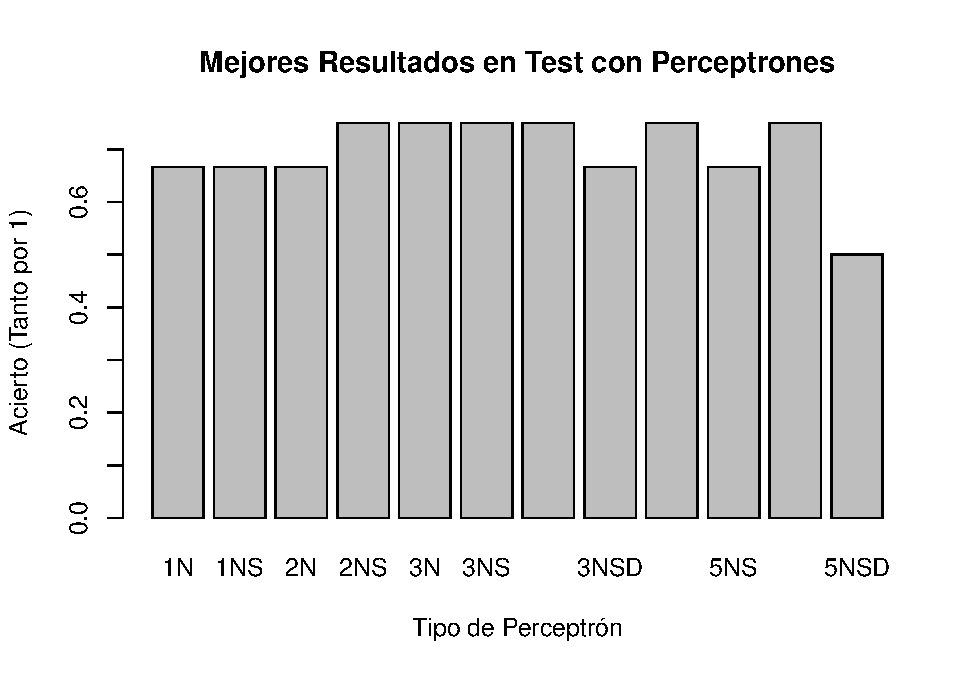
\includegraphics{codigo_files/figure-latex/analisis_resultados_perceptron-1.pdf}

Exporto a PDF este barplot:

\begin{Shaded}
\begin{Highlighting}[]
\KeywordTok{pdf}\NormalTok{(}\StringTok{"Imágenes Obtenidas/BarplotResultadosPerceptron.pdf"}\NormalTok{)}

\KeywordTok{barplot}\NormalTok{(array.maximos.perceptron,}
        \DataTypeTok{main =} \StringTok{"Mejores Resultados en Test con Perceptrones"}\NormalTok{,}
        \DataTypeTok{xlab =} \StringTok{"Tipo de Perceptrón",}
\StringTok{        ylab = "}\KeywordTok{Acierto}\NormalTok{ (Tanto por }\DecValTok{1}\NormalTok{)}\StringTok{",}
\StringTok{        names.arg = c("}\DecValTok{1}\NormalTok{ Neu}\StringTok{", "}\DecValTok{1}\NormalTok{ Neu Soft}\StringTok{", }
\StringTok{                      "}\DecValTok{2}\NormalTok{ Neu}\StringTok{", "}\DecValTok{2}\NormalTok{ Neu Soft}\StringTok{", }
\StringTok{                      "}\DecValTok{3}\NormalTok{ Neu}\StringTok{", "}\DecValTok{3}\NormalTok{ Neu Soft}\StringTok{", "}\DecValTok{3}\NormalTok{ Neu Decay}\StringTok{", "}\DecValTok{3}\NormalTok{ Neu Soft Decay}\StringTok{", }
\StringTok{                      "}\DecValTok{5}\NormalTok{ Neu}\StringTok{", "}\DecValTok{5}\NormalTok{ Neu Soft}\StringTok{", "}\DecValTok{5}\NormalTok{ Neu Decay}\StringTok{", "}\DecValTok{5}\NormalTok{ Neu Soft Decay}\StringTok{")}
\StringTok{      )}

\StringTok{dev.off}
\end{Highlighting}
\end{Shaded}

\begin{verbatim}
## function (which = dev.cur()) 
## {
##     if (which == 1) 
##         stop("cannot shut down device 1 (the null device)")
##     .External(C_devoff, as.integer(which))
##     dev.cur()
## }
## <bytecode: 0x000000001645cb40>
## <environment: namespace:grDevices>
\end{verbatim}

Ahora voy a hacer el mismo dendrograma pero con el DataSet de centrado y
escalado:

\begin{Shaded}
\begin{Highlighting}[]
\KeywordTok{set.seed}\NormalTok{(}\DecValTok{6}\NormalTok{)}

\NormalTok{dd <-}\StringTok{ }\KeywordTok{dist}\NormalTok{(}\KeywordTok{scale}\NormalTok{(matriz.pacientes.datos.centscal), }\DataTypeTok{method =} \StringTok{"euclidean"}\NormalTok{)}
\NormalTok{hier.clust <-}\StringTok{ }\KeywordTok{hclust}\NormalTok{(dd, }\DataTypeTok{method =} \StringTok{"ward.D2"}\NormalTok{)}
\NormalTok{colores.dendrograma <-}\StringTok{ }\KeywordTok{c}\NormalTok{(}\StringTok{"red"}\NormalTok{, }\StringTok{"orange"}\NormalTok{, }\StringTok{"green"}\NormalTok{, }\StringTok{"black"}\NormalTok{)}
\NormalTok{cluster}\FloatTok{.4}\NormalTok{ <-}\StringTok{ }\KeywordTok{cutree}\NormalTok{(hier.clust, }\DecValTok{4}\NormalTok{)}
\KeywordTok{plot}\NormalTok{(}\KeywordTok{as.phylo}\NormalTok{(hier.clust), }\DataTypeTok{type =} \StringTok{"fan"}\NormalTok{, }\DataTypeTok{tip.color =}\NormalTok{ colores.dendrograma[cluster}\FloatTok{.4}\NormalTok{], }\DataTypeTok{label.offset =} \FloatTok{0.3}\NormalTok{, }\DataTypeTok{cex =} \FloatTok{0.8}\NormalTok{)}
\end{Highlighting}
\end{Shaded}

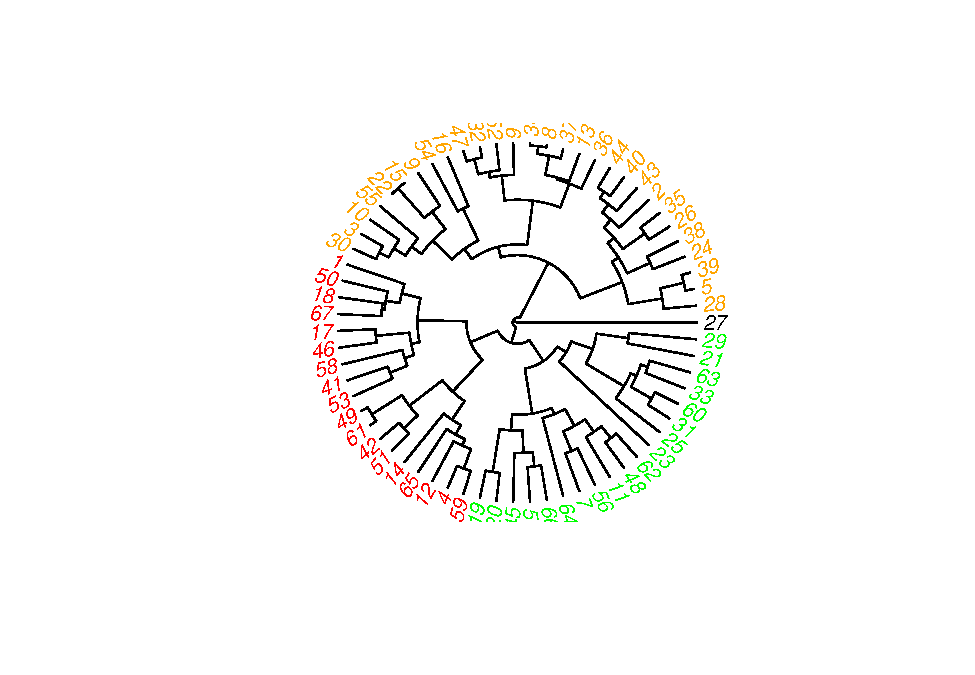
\includegraphics{codigo_files/figure-latex/creacion_clusters_dendrograma_centradoEscalado-1.pdf}

Lo exportamos a PDF tras la creación:

\begin{Shaded}
\begin{Highlighting}[]
\KeywordTok{pdf}\NormalTok{(}\StringTok{"Imágenes Obtenidas/dendrograma_pacientes_centscal.pdf"}\NormalTok{)}

\KeywordTok{plot}\NormalTok{(}\KeywordTok{as.phylo}\NormalTok{(hier.clust), }\DataTypeTok{type =} \StringTok{"fan"}\NormalTok{, }\DataTypeTok{tip.color =}\NormalTok{ colores.dendrograma[cluster}\FloatTok{.4}\NormalTok{], }\DataTypeTok{label.offset =} \FloatTok{0.3}\NormalTok{, }\DataTypeTok{cex =} \FloatTok{0.8}\NormalTok{)}

\KeywordTok{dev.off}\NormalTok{()}
\end{Highlighting}
\end{Shaded}


\end{document}
